\subsubsection{Skipping on sequential switching between Tent and Logistic maps (EVEN and ODD)} \label{sssec:skipp}

Skipping is a usual randomizing technique that increases the mixing quality of a single map and correspondingly increases the value of $H_{BP}$ and decreases $C_{BP} $ of the time series.
Skipping does not change the values of $H_{val}$ and $C_{val}$ evaluated using the non causal PDF (normalized histogram of values)\cite{DeMicco2008}.

In the case under consideration we study Even and Odd skipping of the sequential switching of Tent and Logistic maps:
\begin{enumerate}
	\item Even skipping of the sequential switching of Tent and Logistic maps (EVEN).\\
	If $\{x_n,~(n=1,...\infty)\}$ is the time series generated by \ref{eq:SWITCH}, discard all the values in odd positions and retain the values in even positions.
	\item Odd skipping of the sequential switching of Tent and Logistic maps.
	If $\{x_n,~(n=1,...\infty)\}$ is the time series generated by \ref{eq:SWITCH}, discard all the values in even positions and retain all the values in odd positions.
\end{enumerate}

\begin{figure}
	\includegraphics[height=0.4\textheight]{SwitchParImpar}
	\caption{Sequential switching between Tent and Logistic maps. In the figure are also shown even and odd skipping strategies.} \label{fig:seq}
\end{figure}

The reason for studying even and odd skipping cases is the sequential switching map $M_{switch}$ is the composition of two different maps. Even skipping may be expressed as $M_{TENT}\circ M_{LOG}$ while odd skipping may be expressed as $M_{LOG} \circ M_{TENT}$.
The evolution of period as function of precision was reported in \cite{Nagaraj2008}.

In the figures \ref{fig:EVEN_QuantiB}.a and \ref{fig:ODD_QuantiB}.a, quantifiers related to the normalized histogram of values slightly degrades with the skipping procedure due to finite data length.
For example $H_{val}$ reduces from $0.9722$ without skipping to $0.9459$ for EVEN and $0.9706$ for ODD. 
This difference between EVEN and ODD in floating point is because an high dispersion was obtained for $H_{val}$, $H_{BP}$ and $C_{BP}$ but not for $H_{BPW}$ or $C_{BPW}$.
\textcolor{red}{VER LOS ATRACTORES Y EXPLICAR, ADEMÁS REVISAR CÓDIGO}


Figs. \ref{fig:EVEN_QuantiB}.b to \ref{fig:EVEN_QuantiB}.f. and Figs. \ref{fig:ODD_QuantiB}.b to \ref{fig:ODD_QuantiB}.f show the results of $BP$ and $BPW$ quantifiers for EVEN and ODD respectively.
Higher accuracy is required to achieve lower complexity than without using skipping.
From the point of view of order patterns a great improvement is obtained using any of the skipping strategies but ODD is slightly better than EVEN.
MP are reduced to $MP\simeq 118$ for EVEN and  ODD, increasing the maximum allowed Bandt \& Pompe entropy that reaches the mean value $<H_{BP}> = 0.8381$ for EVEN, and $<H_{BP}> = 0.9094$.
The complexity is reduced to $<C_{BP}>\simeq 0.224$ for EVEN and  $<C_{BP}>\simeq 0.282$ for ODD.
The amount of bits necessary to converge to this value is $B>40$ for both EVEN and ODD maps.

\begin{figure}
	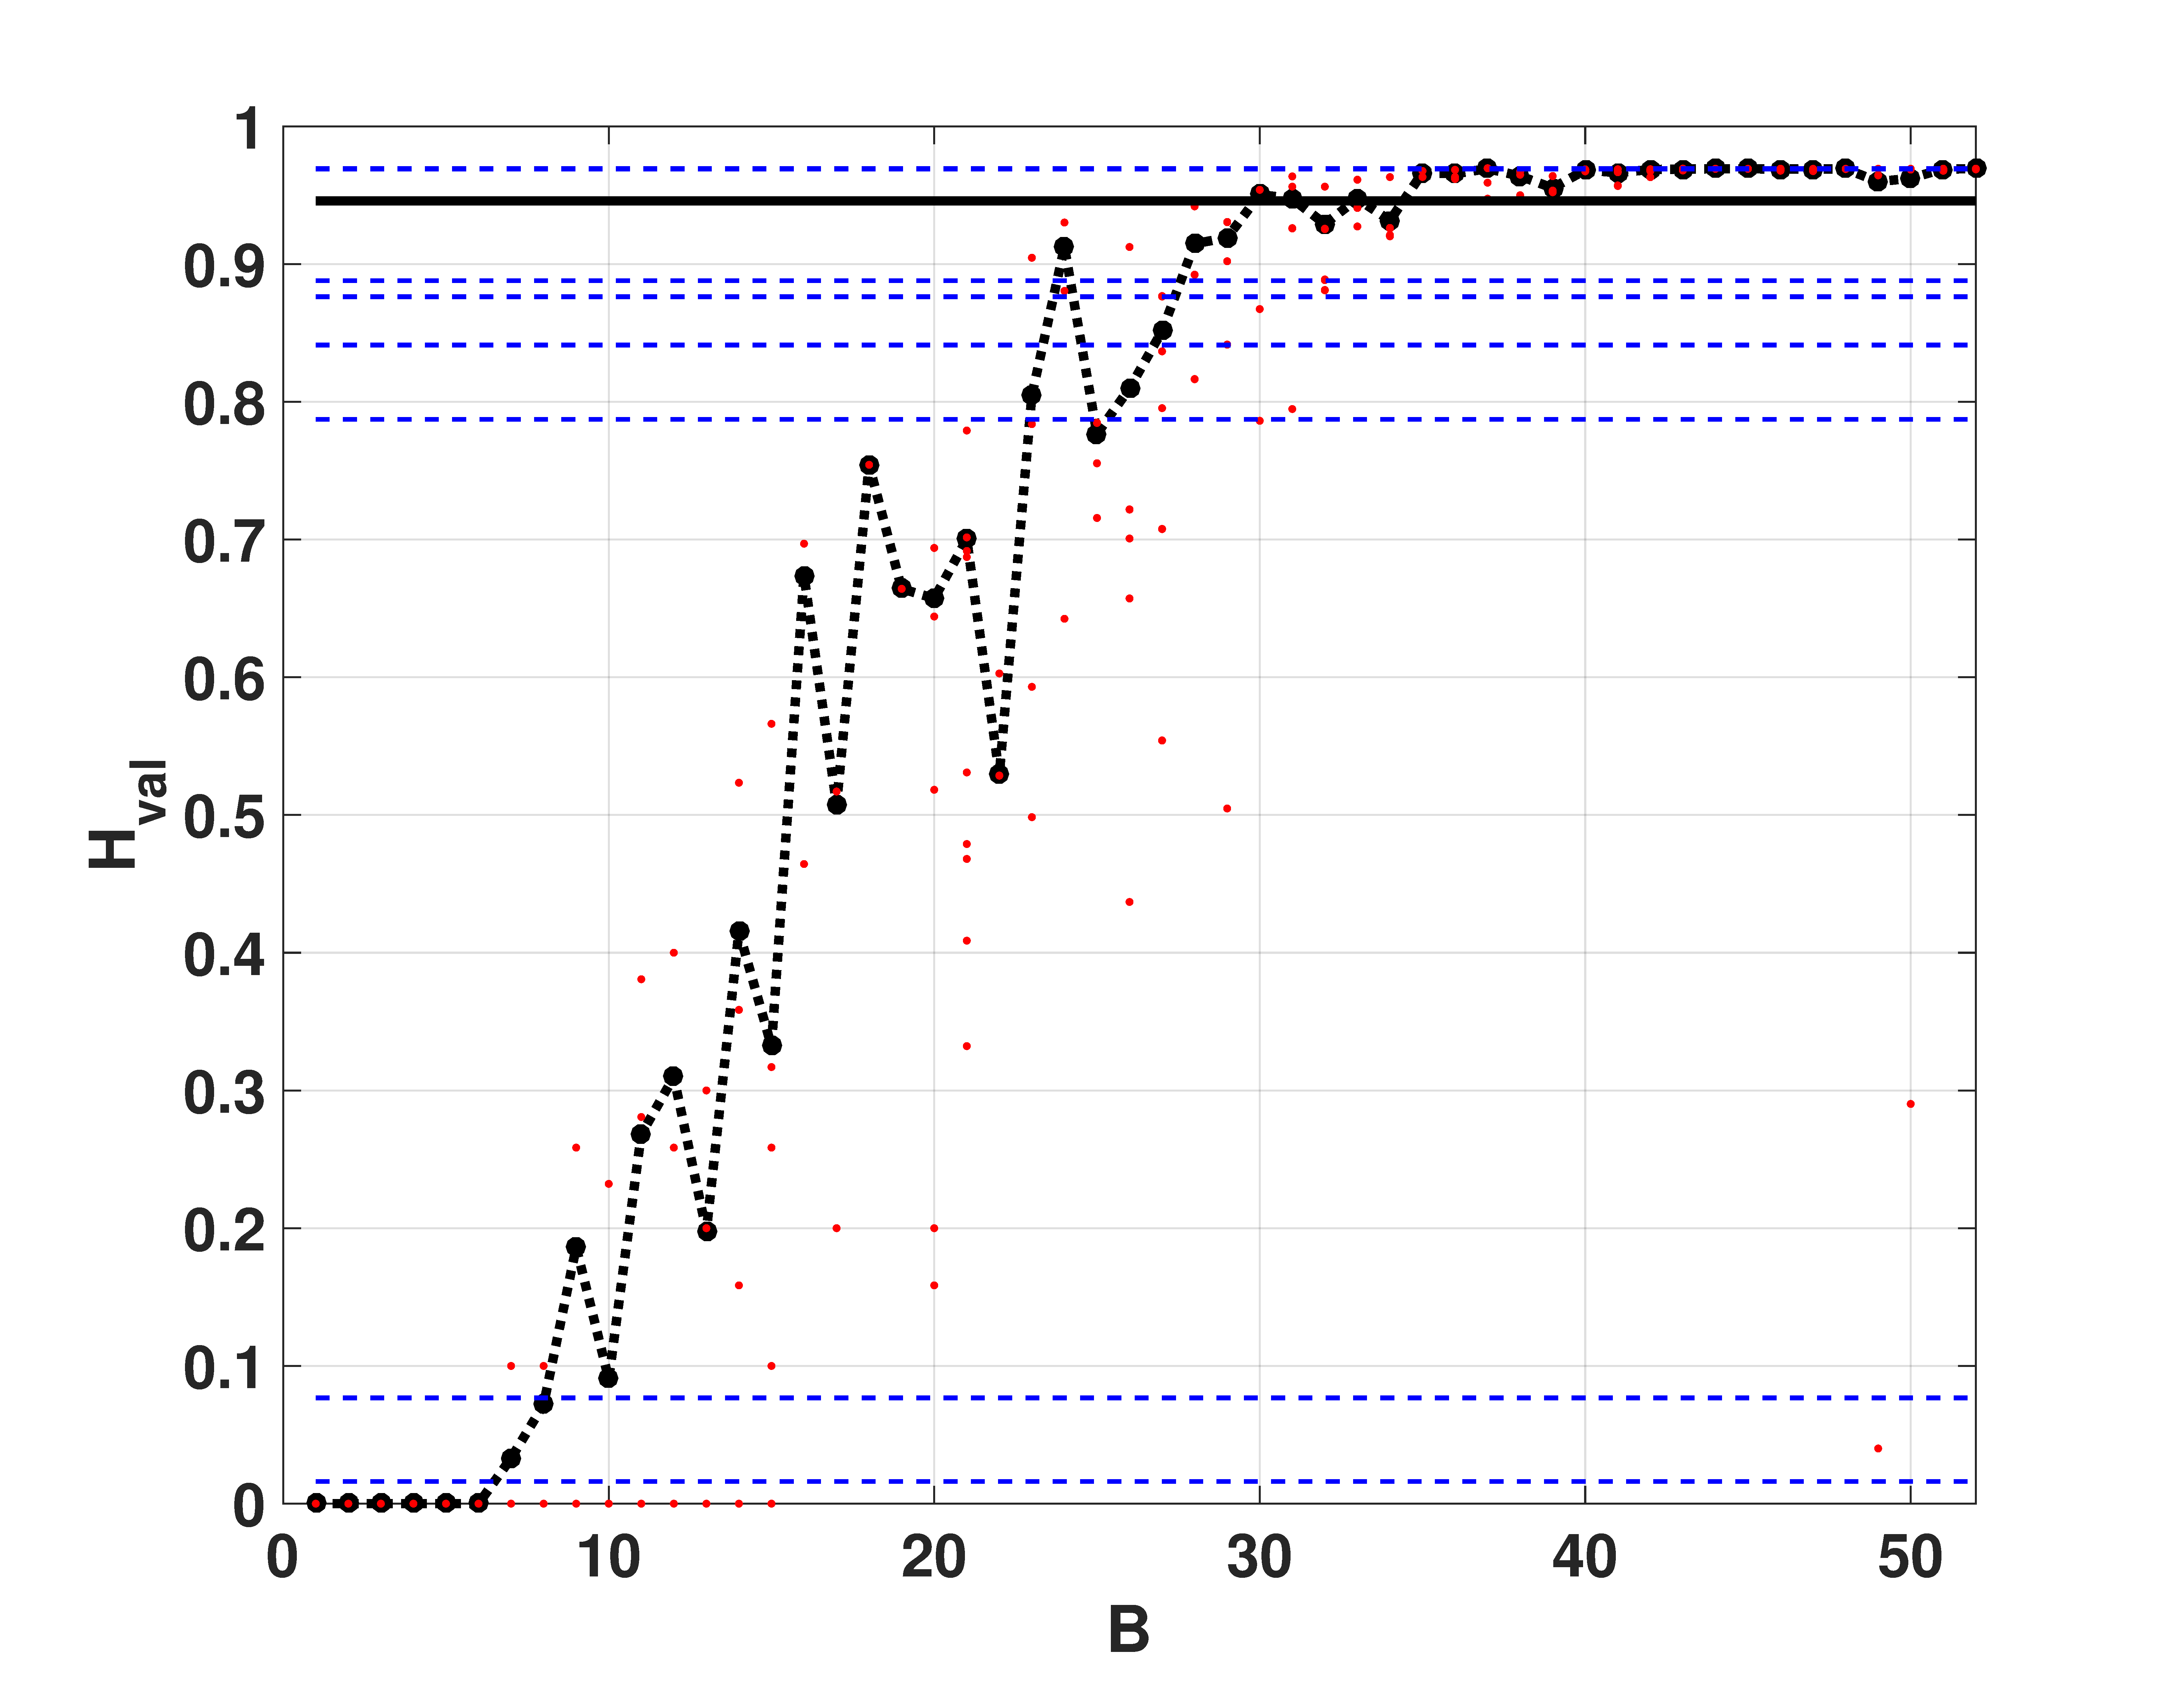
\includegraphics[width=.49\textwidth]{Hval_SwitchEven}
	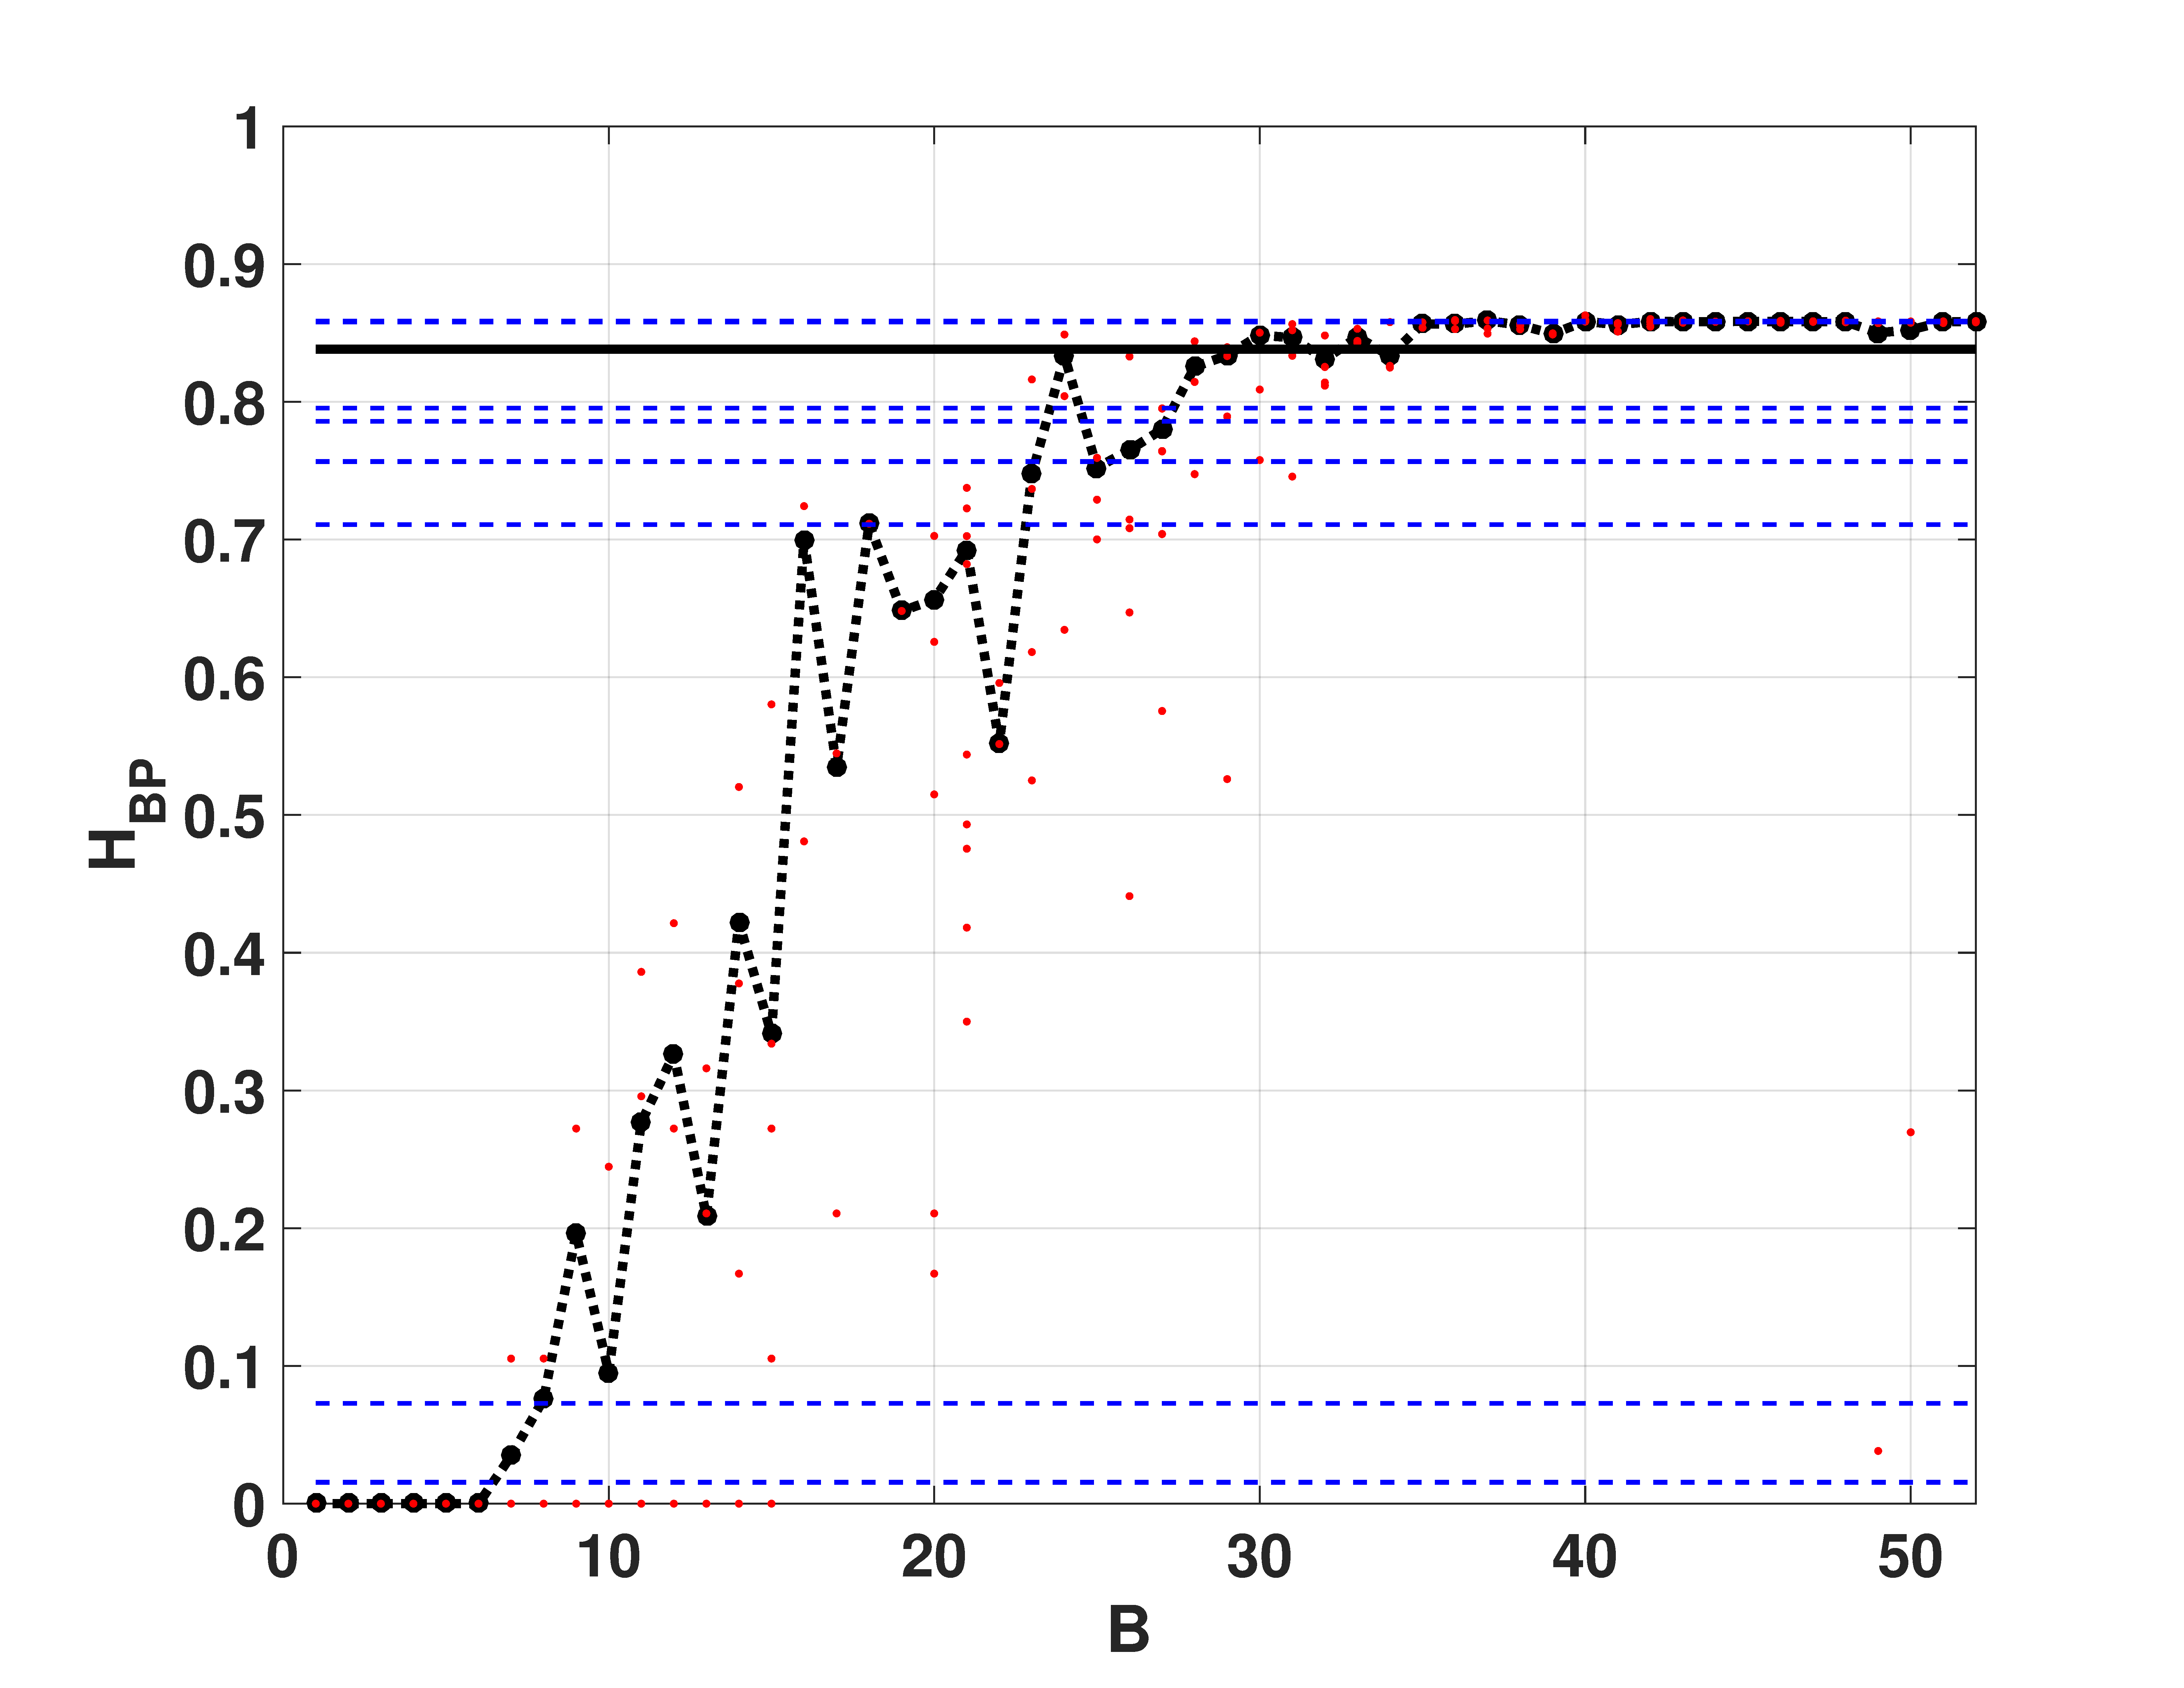
\includegraphics[width=.49\textwidth]{Hbp_SwitchEven}
	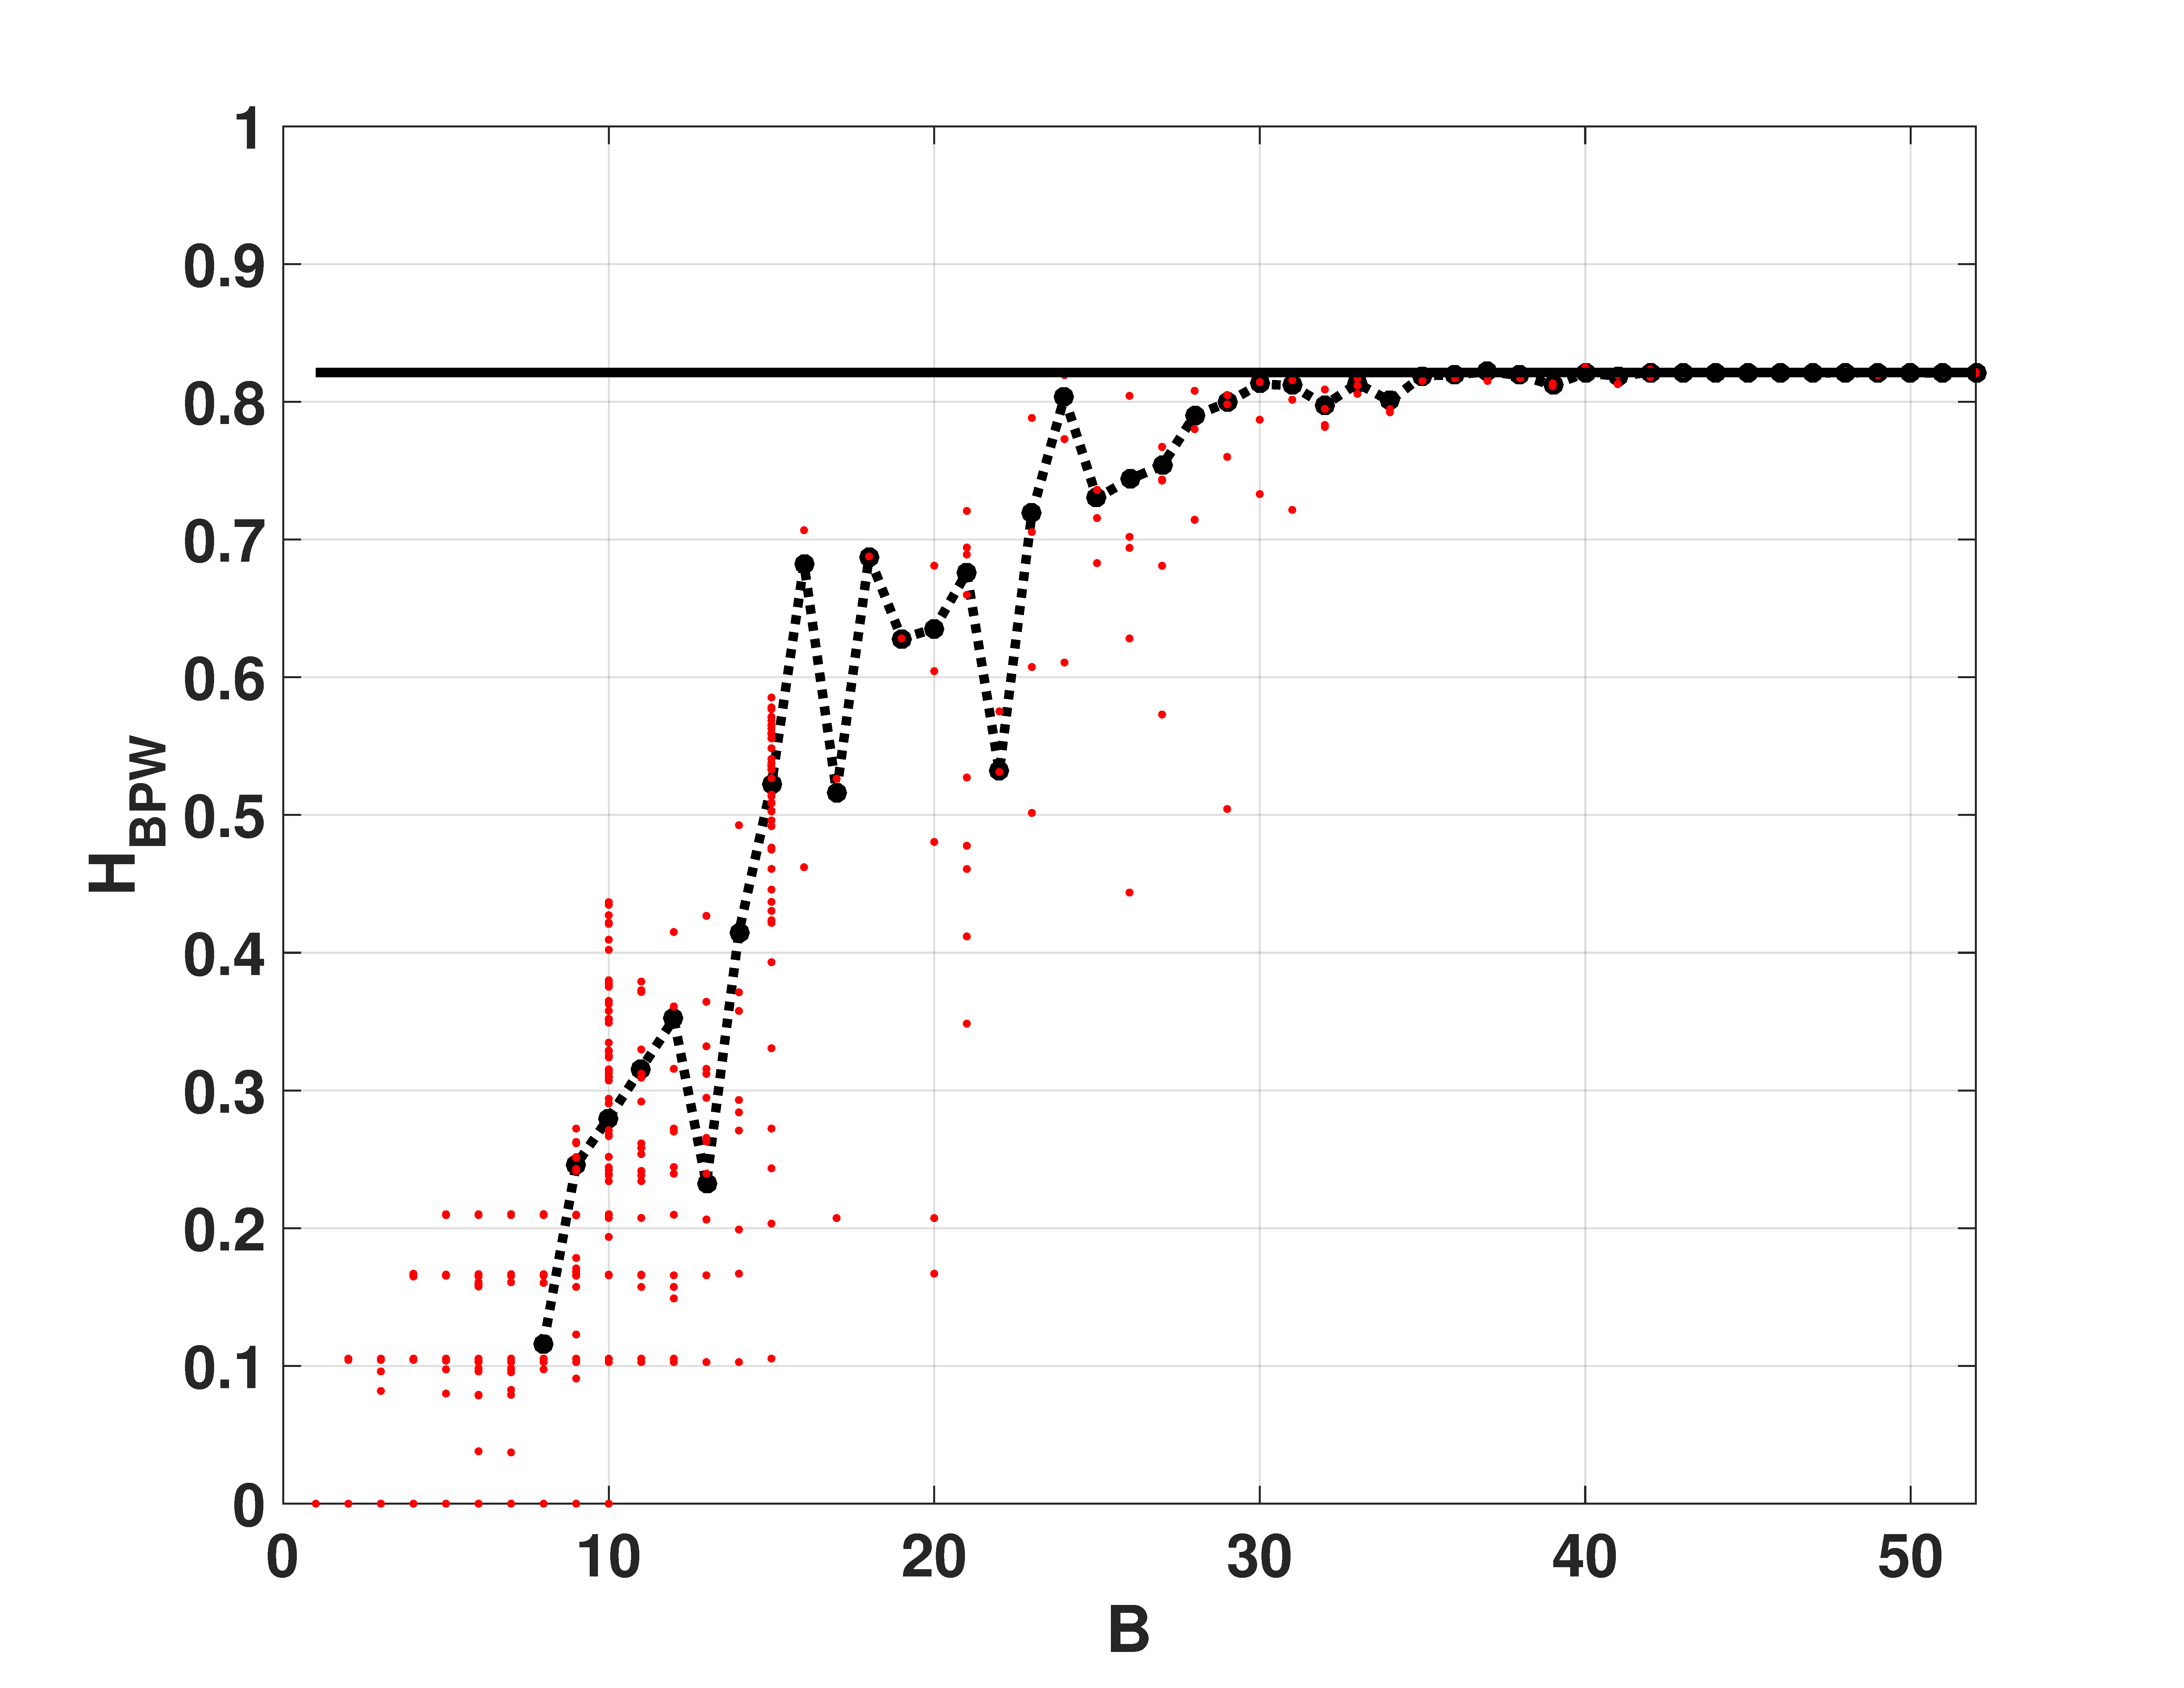
\includegraphics[width=.49\textwidth]{Hbpw_SwitchEven}
	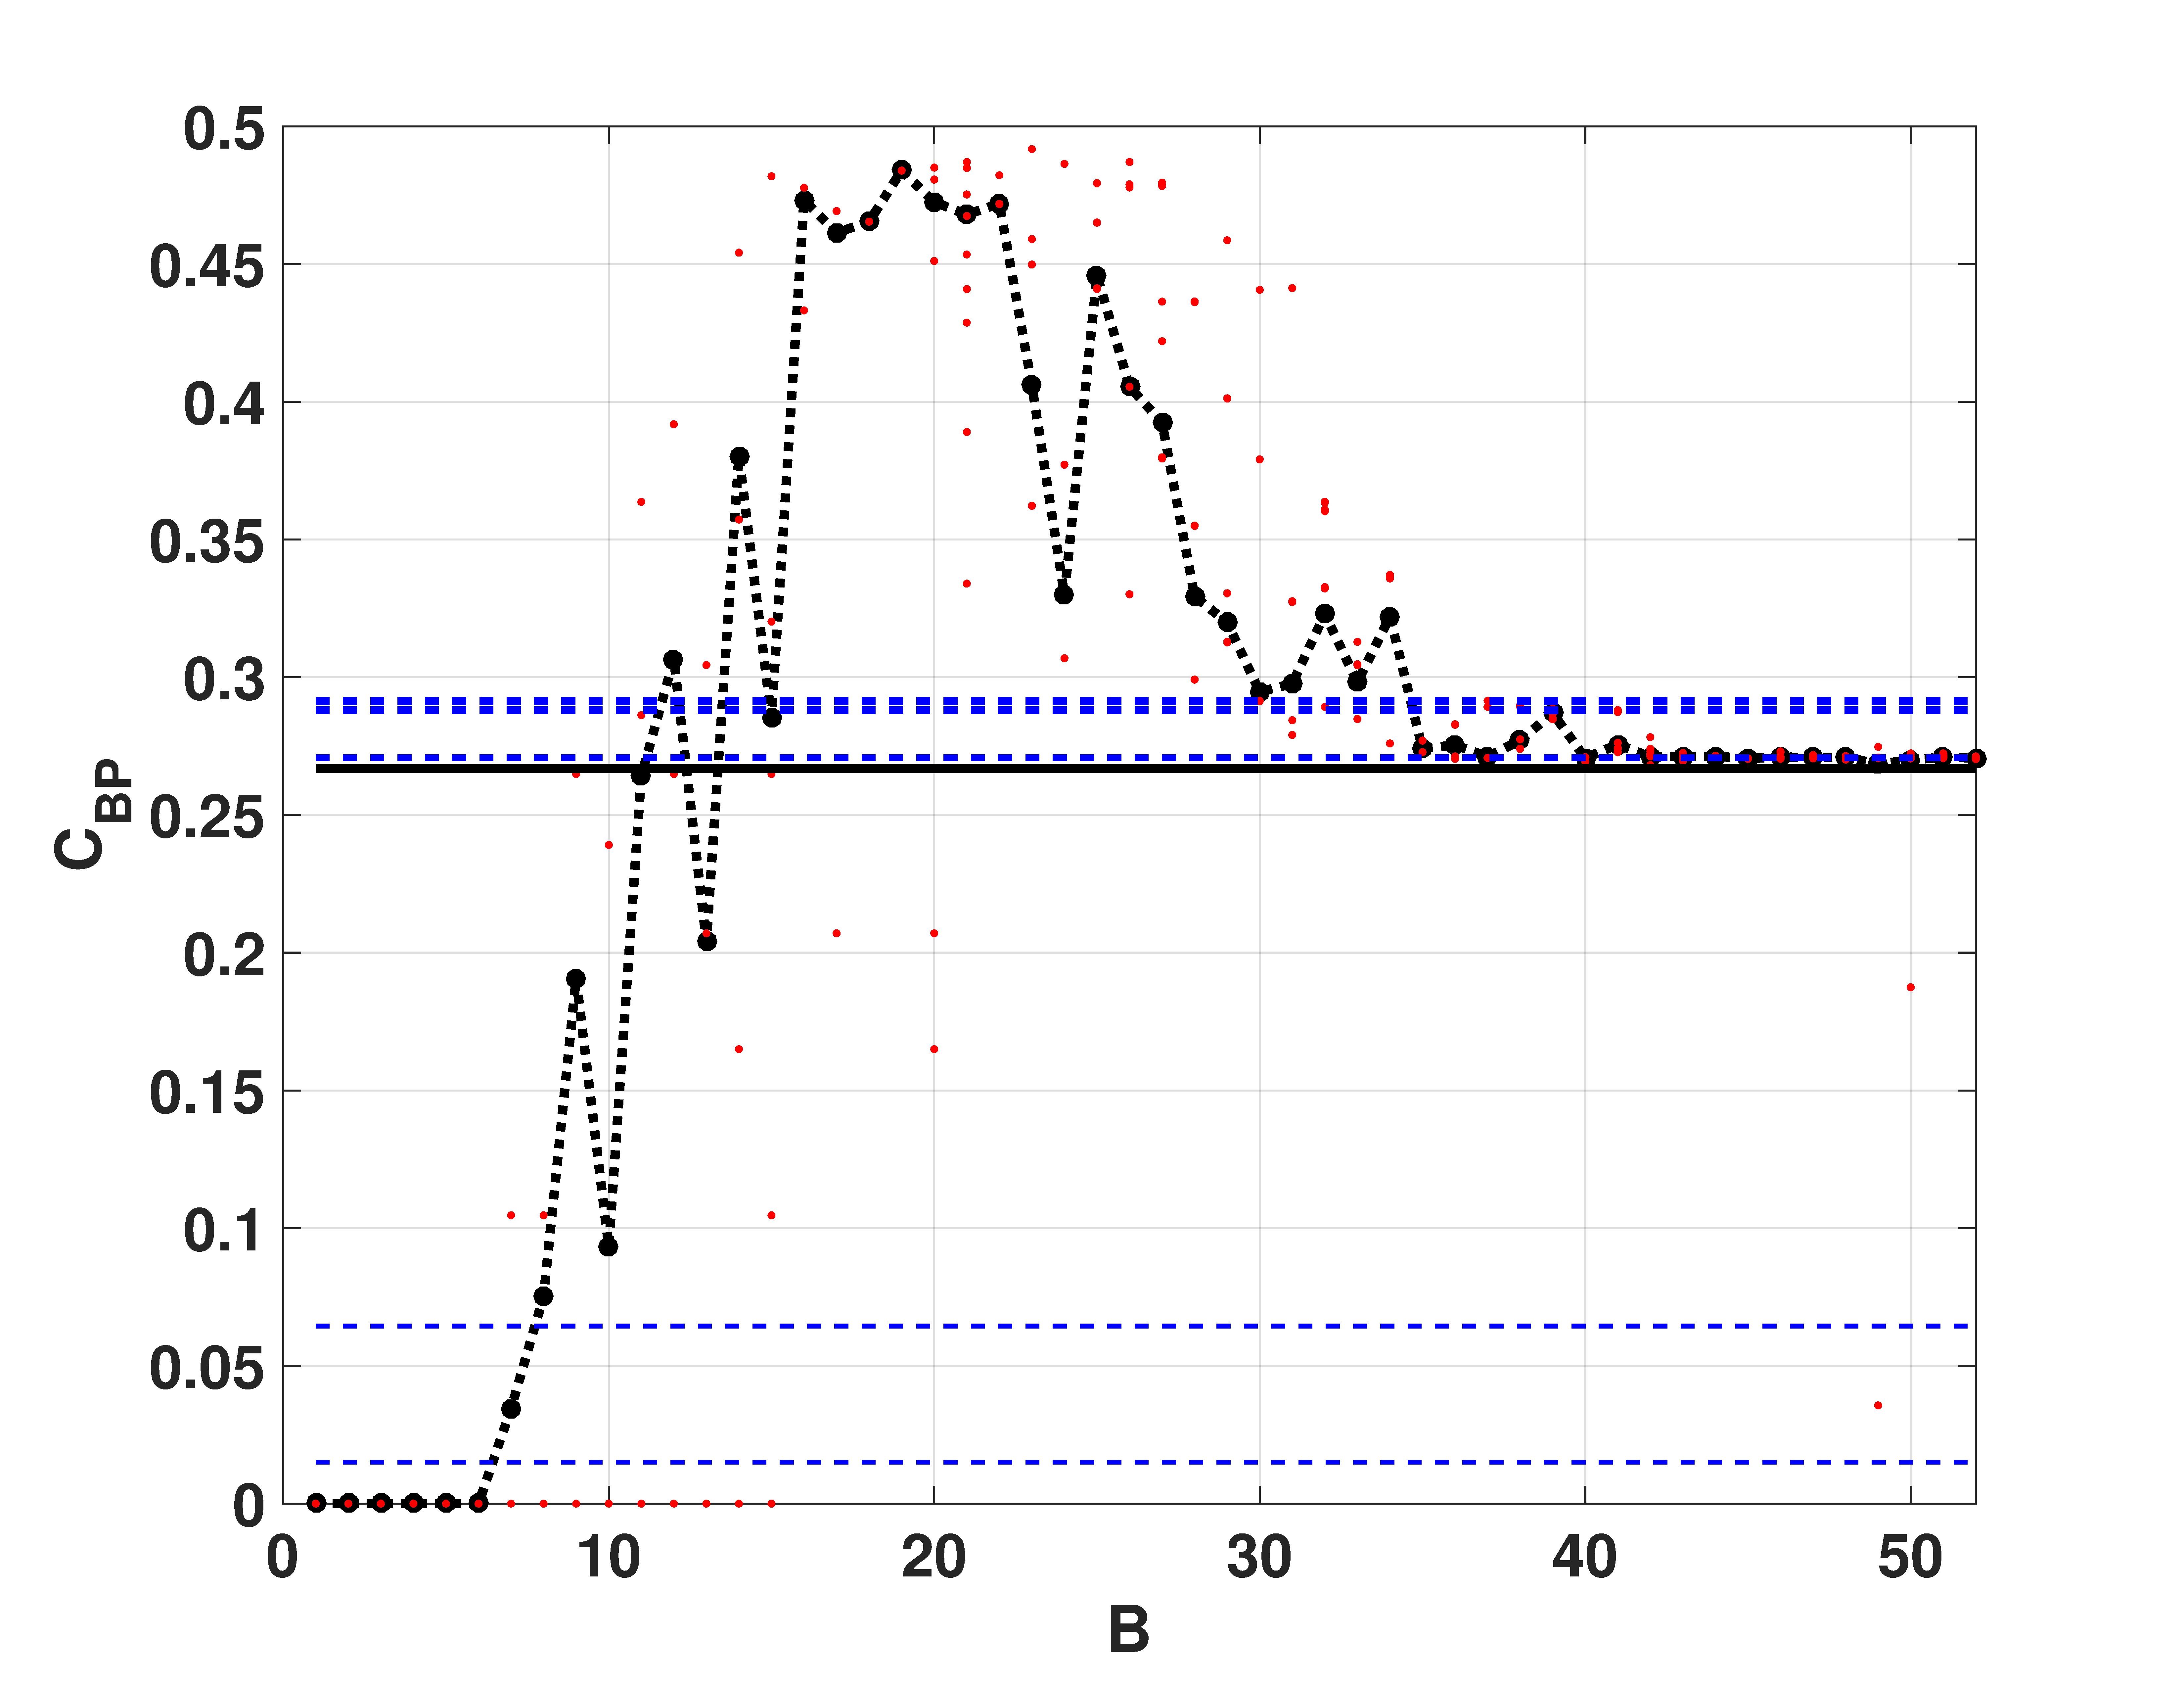
\includegraphics[width=.49\textwidth]{Cbp_SwitchEven}
	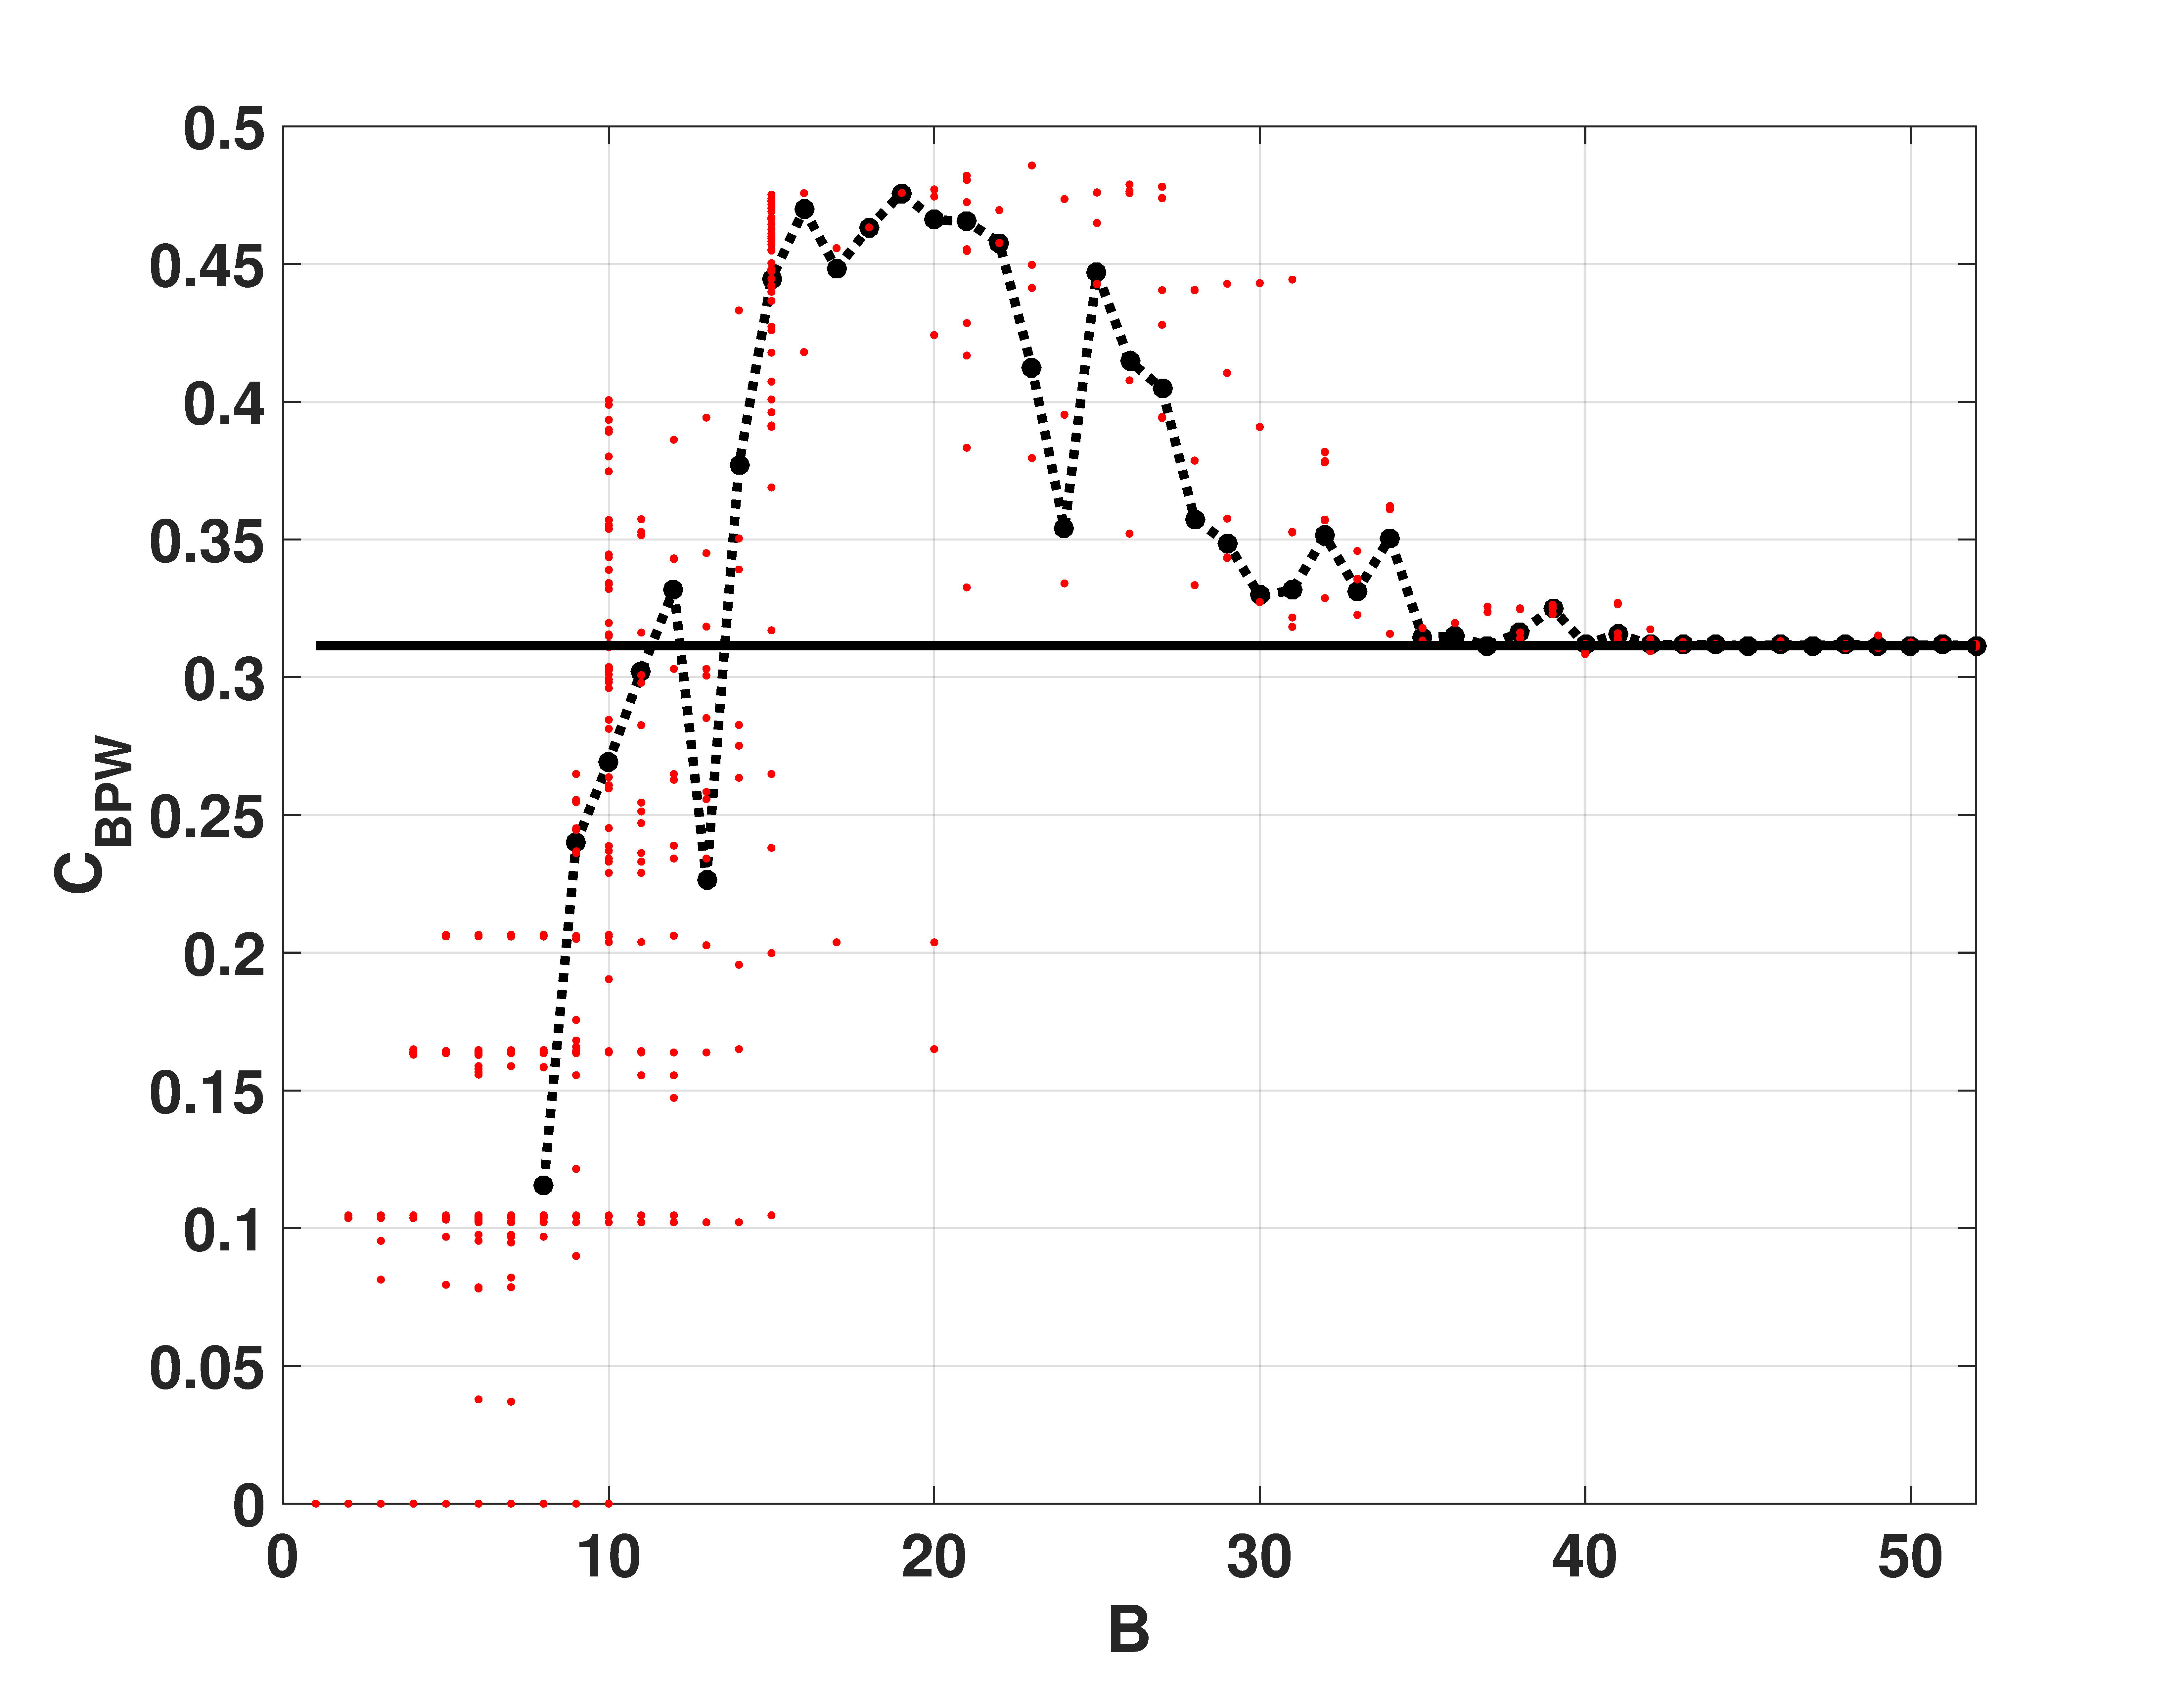
\includegraphics[width=.49\textwidth]{Cbpw_SwitchEven}
	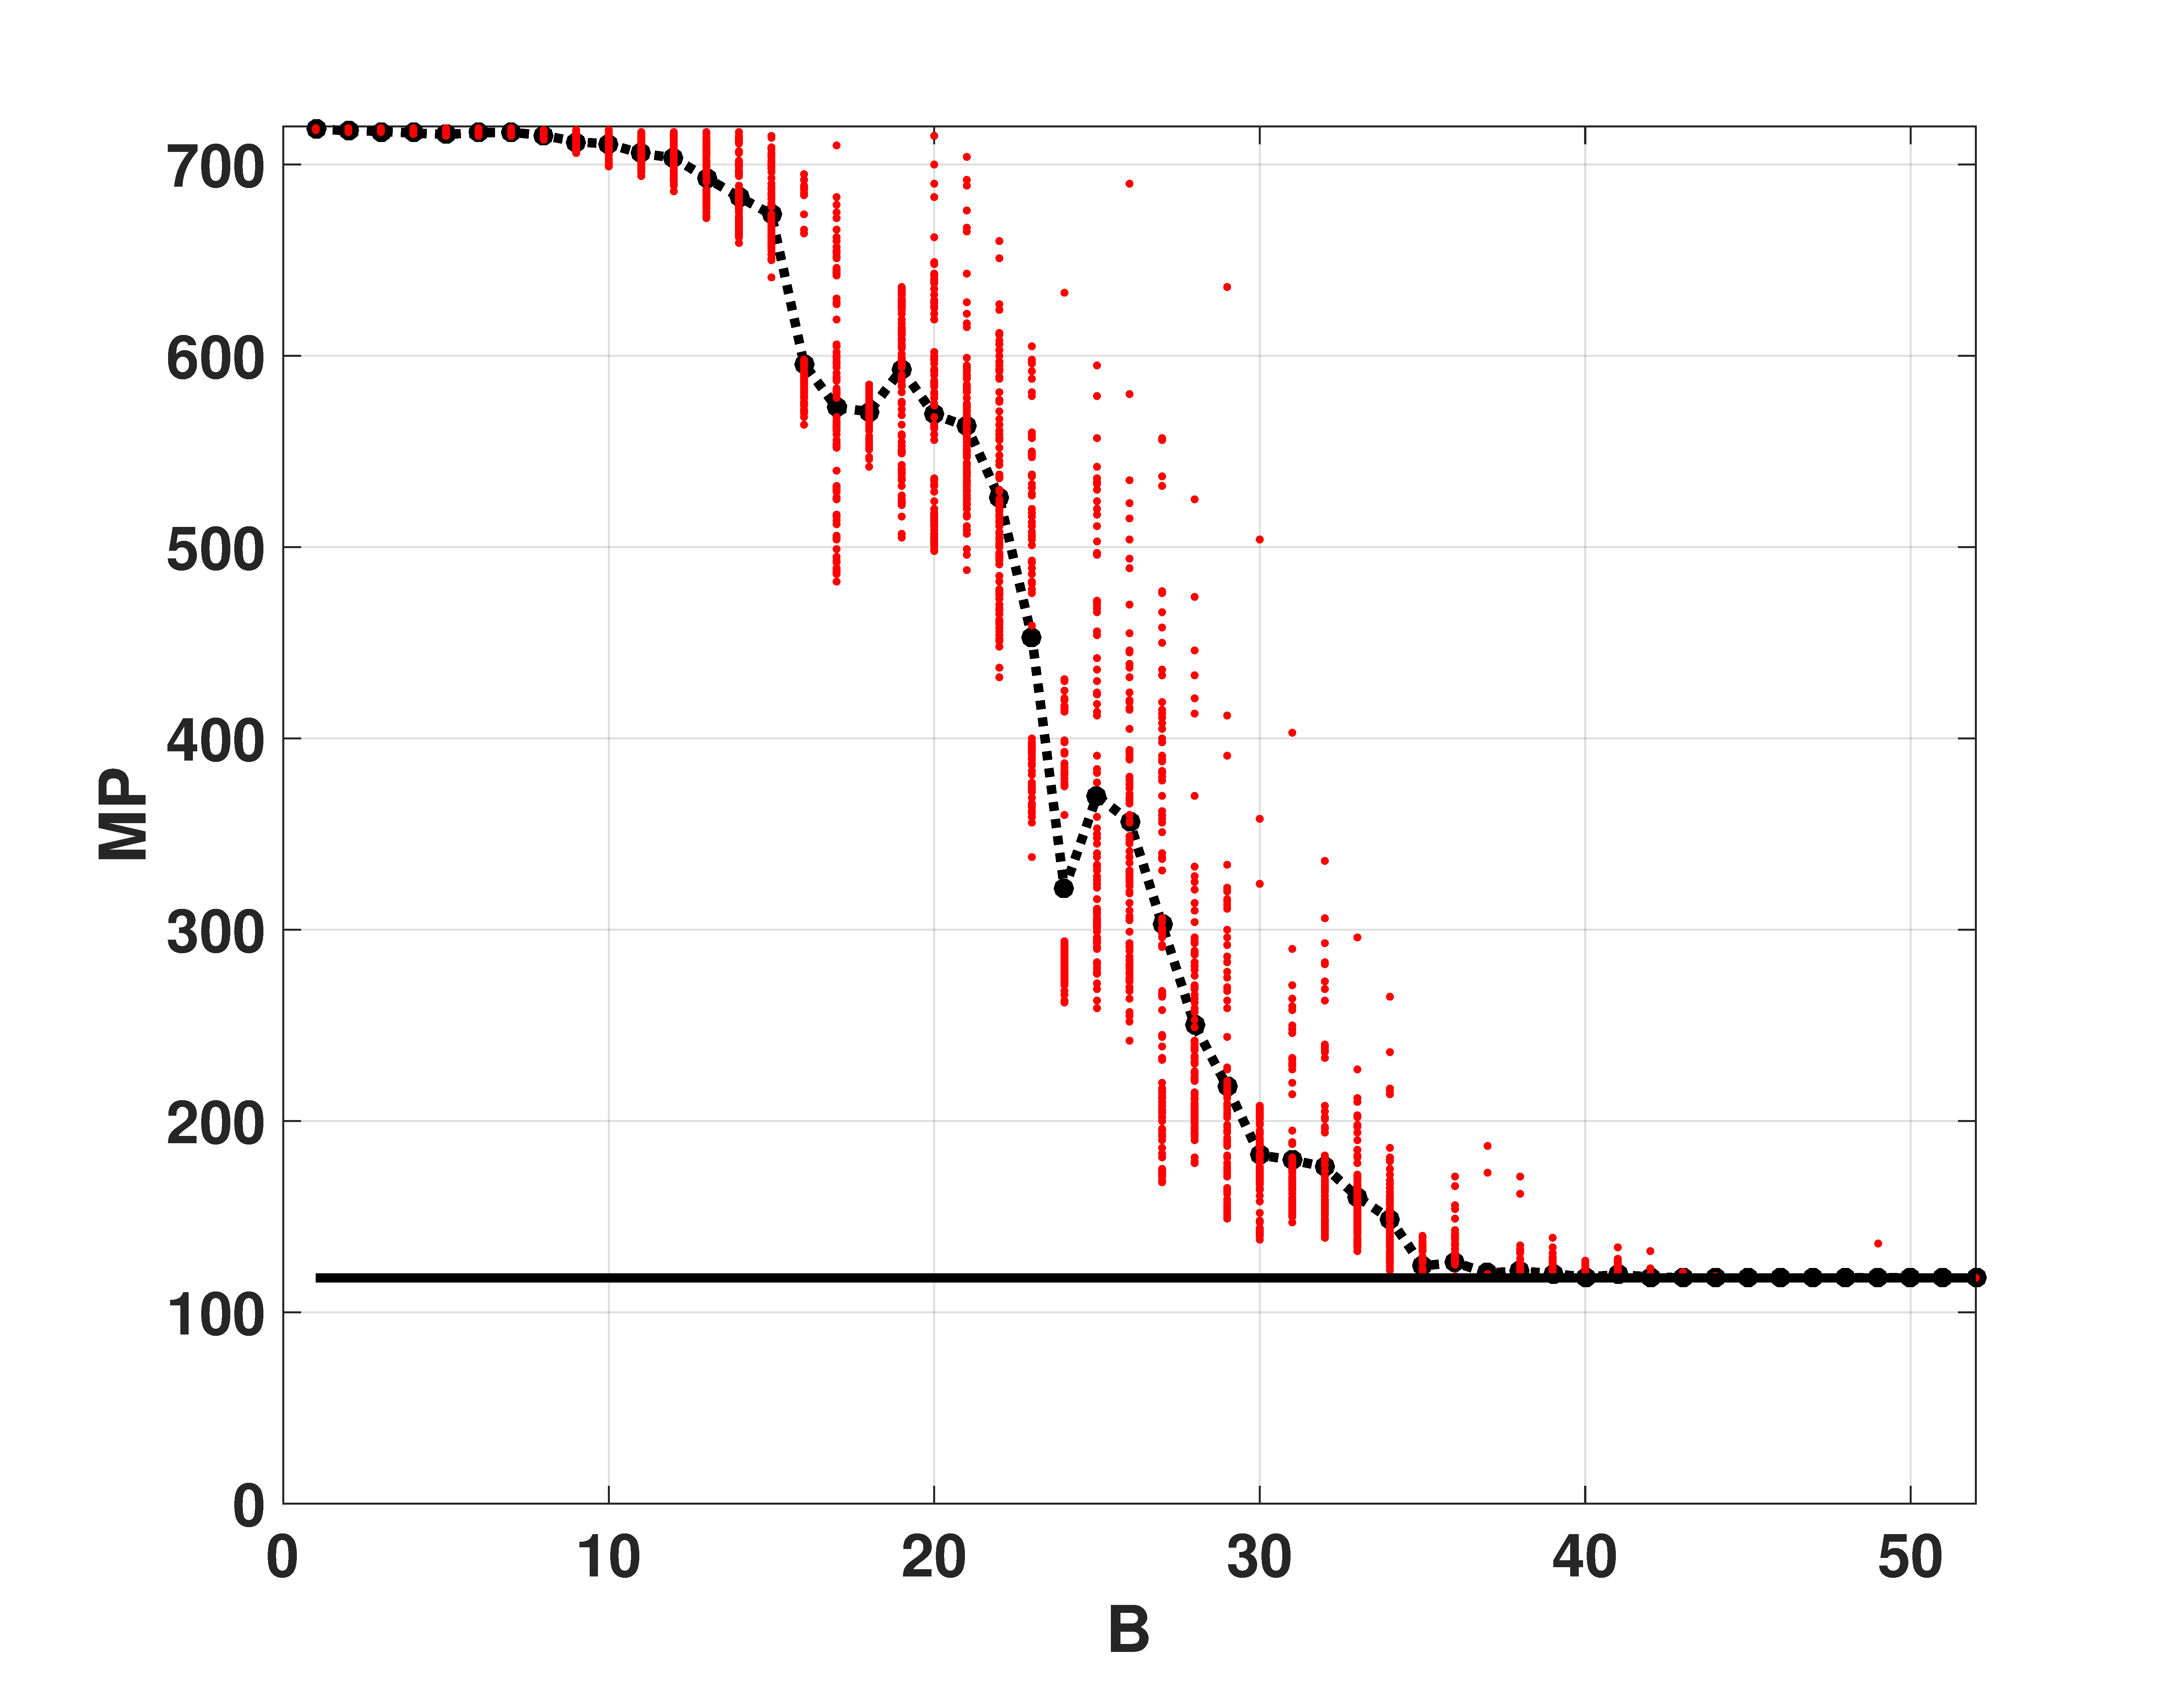
\includegraphics[width=.49\textwidth]{MP_SwitchEven}
	\caption{Statistical properties of the EVEN map using binary representation: (a) $H_{val}$ vs $B$ (b) $H_{BP}$ vs $B$ (c) $C_{BP}$ vs $B$ (d) Number of missing ordering patterns $MP$ vs $B$.}
	\label{fig:EVEN_QuantiB}
\end{figure}

\begin{figure}
	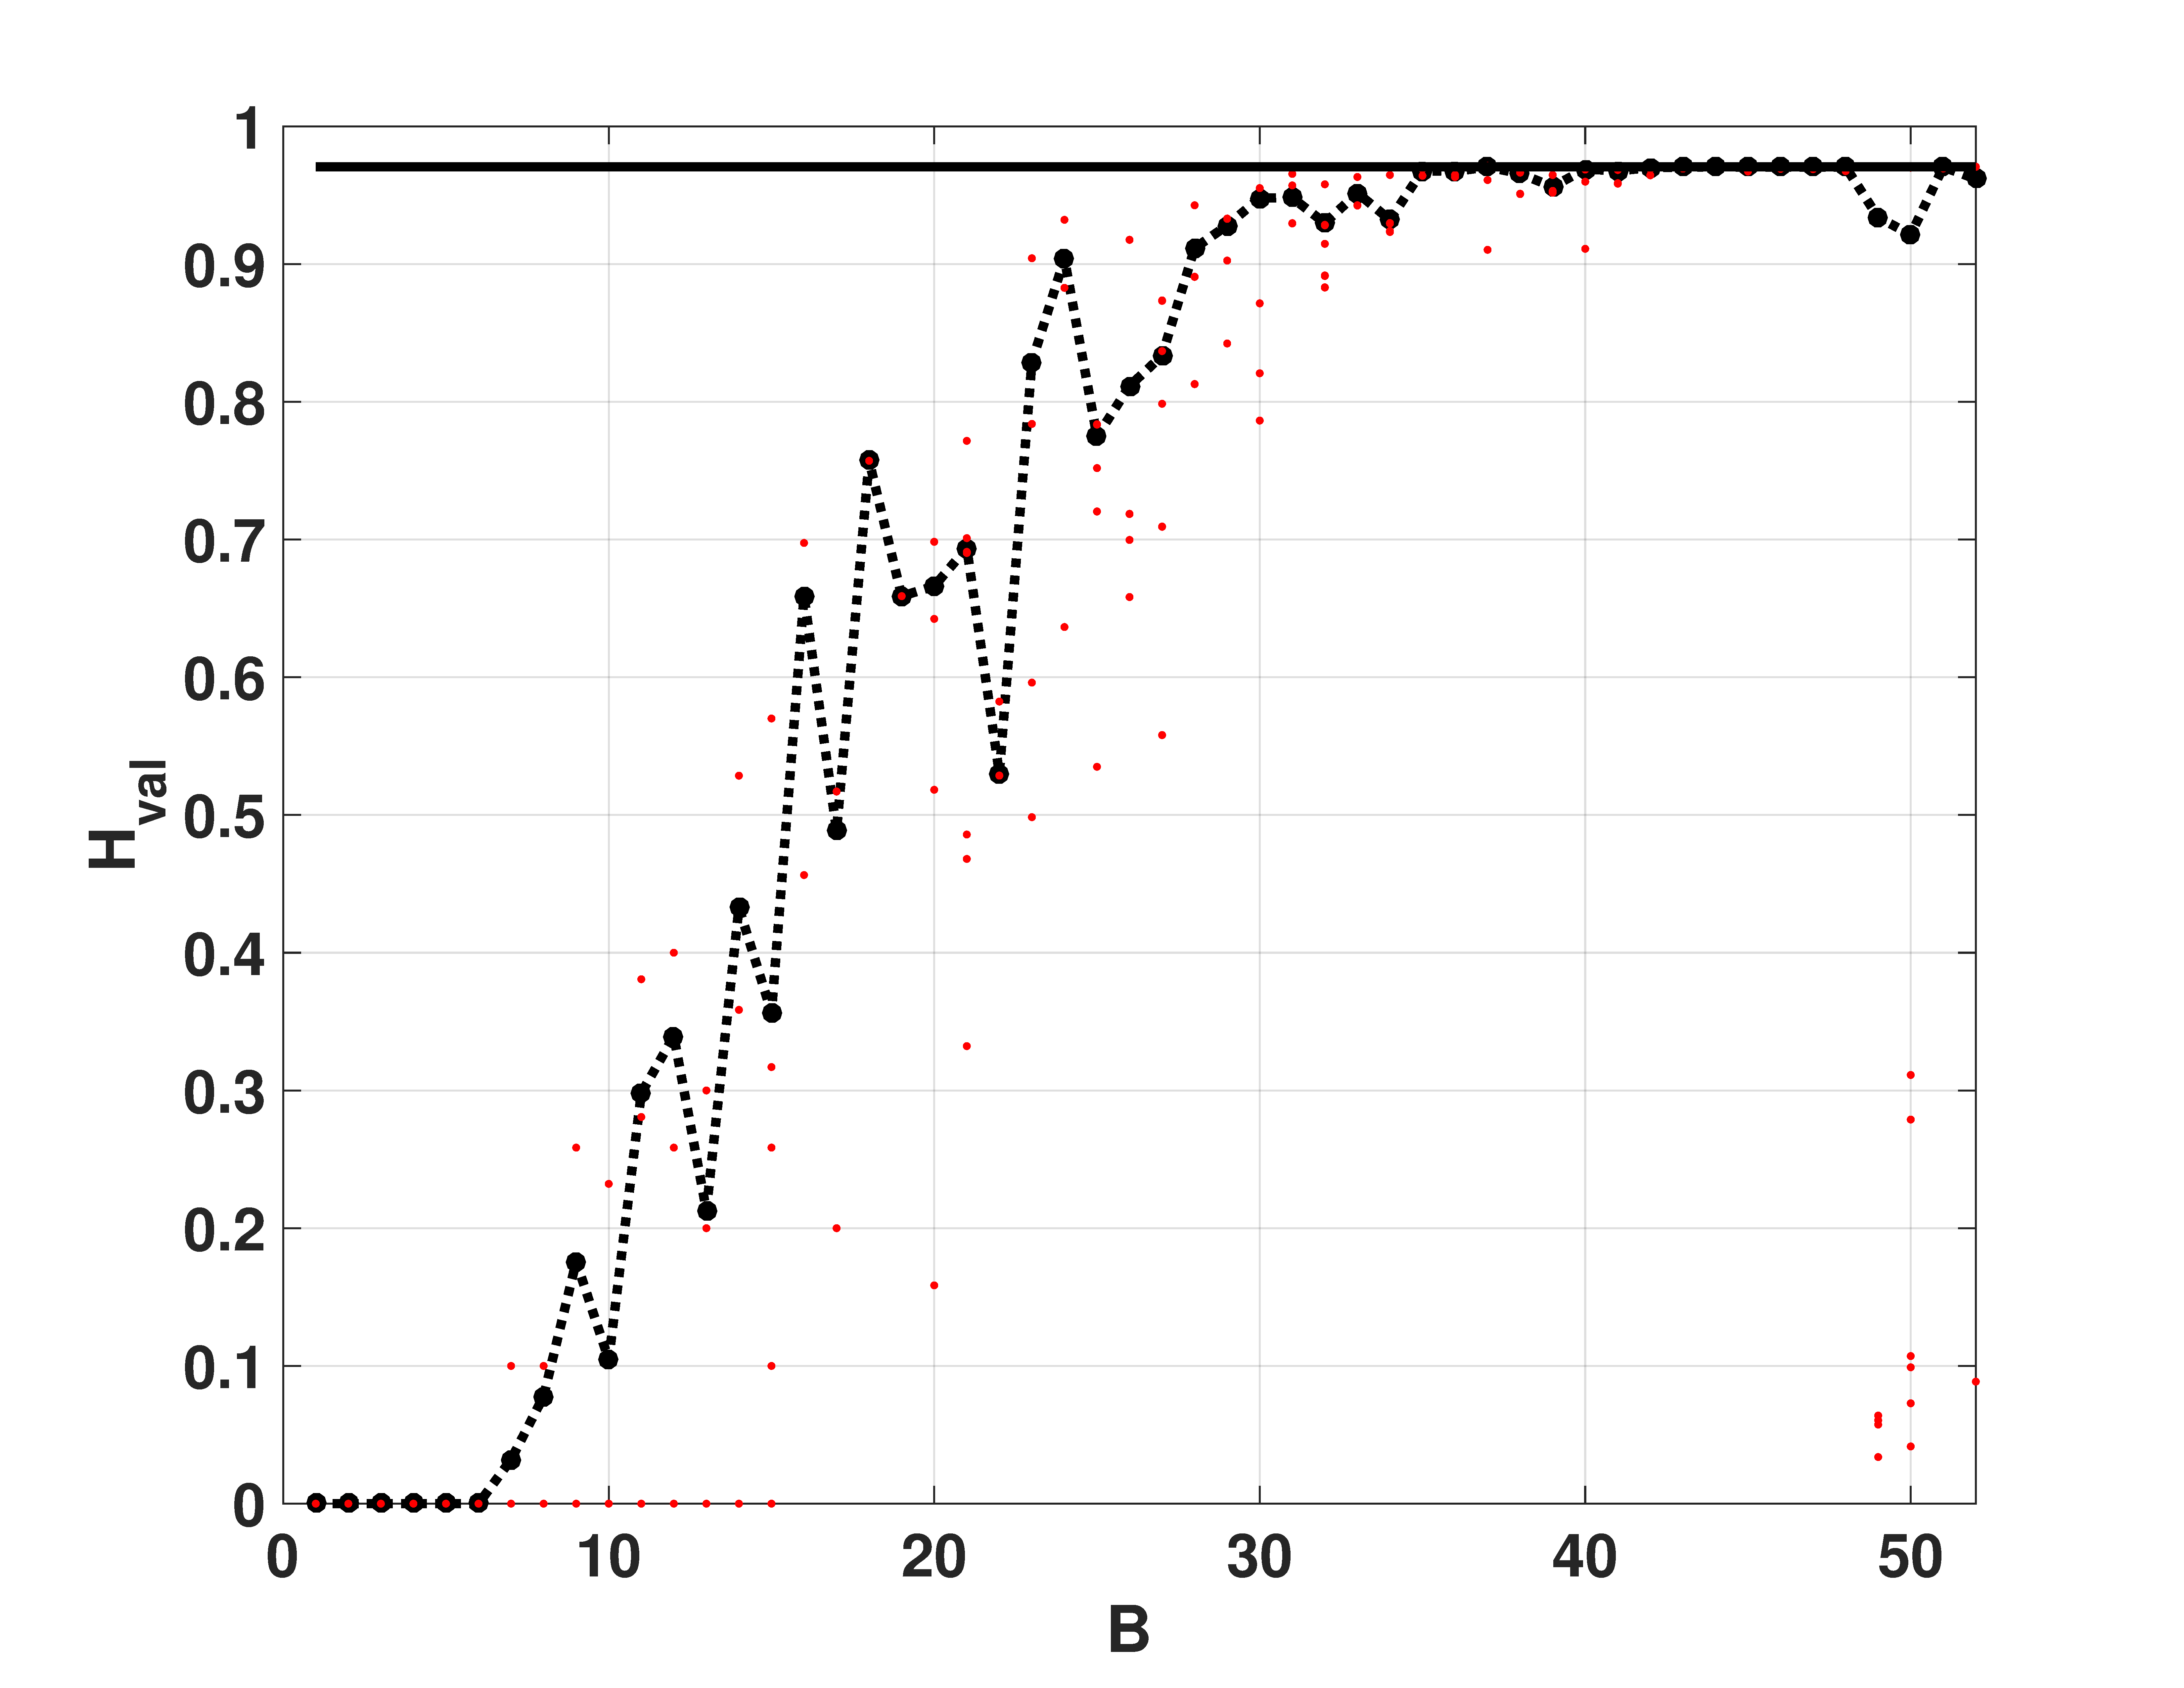
\includegraphics[width=.49\textwidth]{Hval_SwitchOdd}
	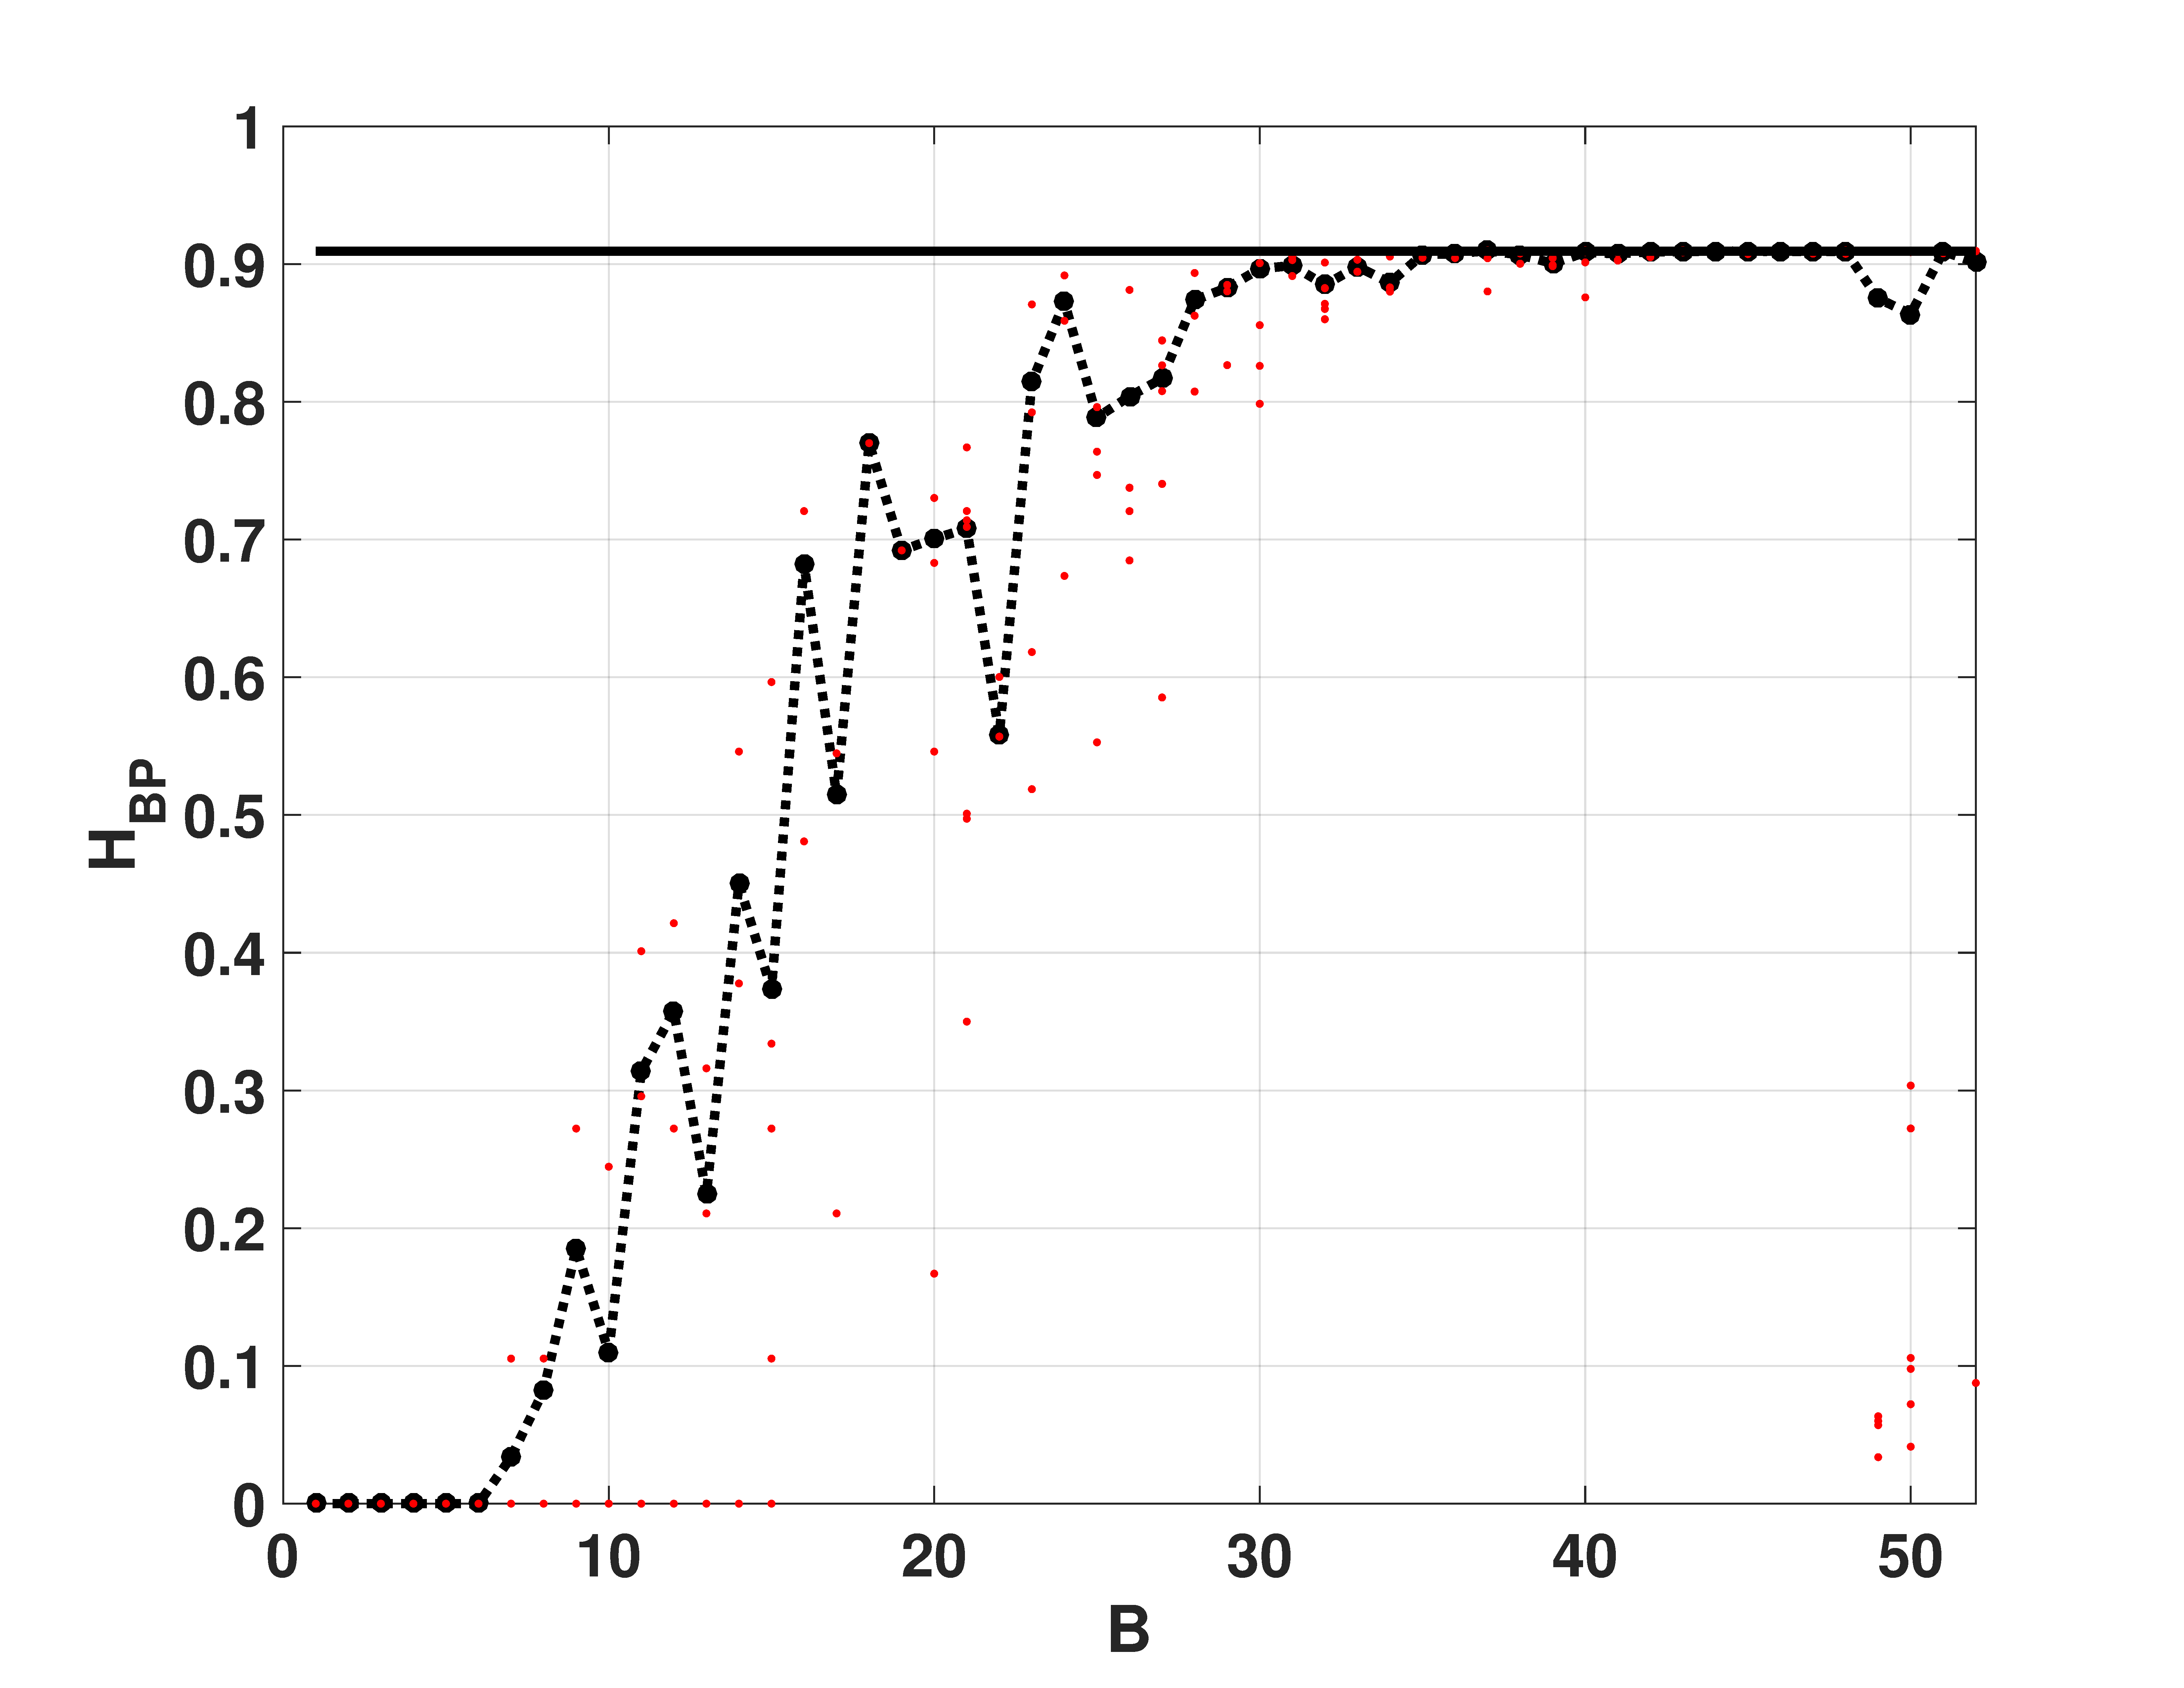
\includegraphics[width=.49\textwidth]{Hbp_SwitchOdd}
	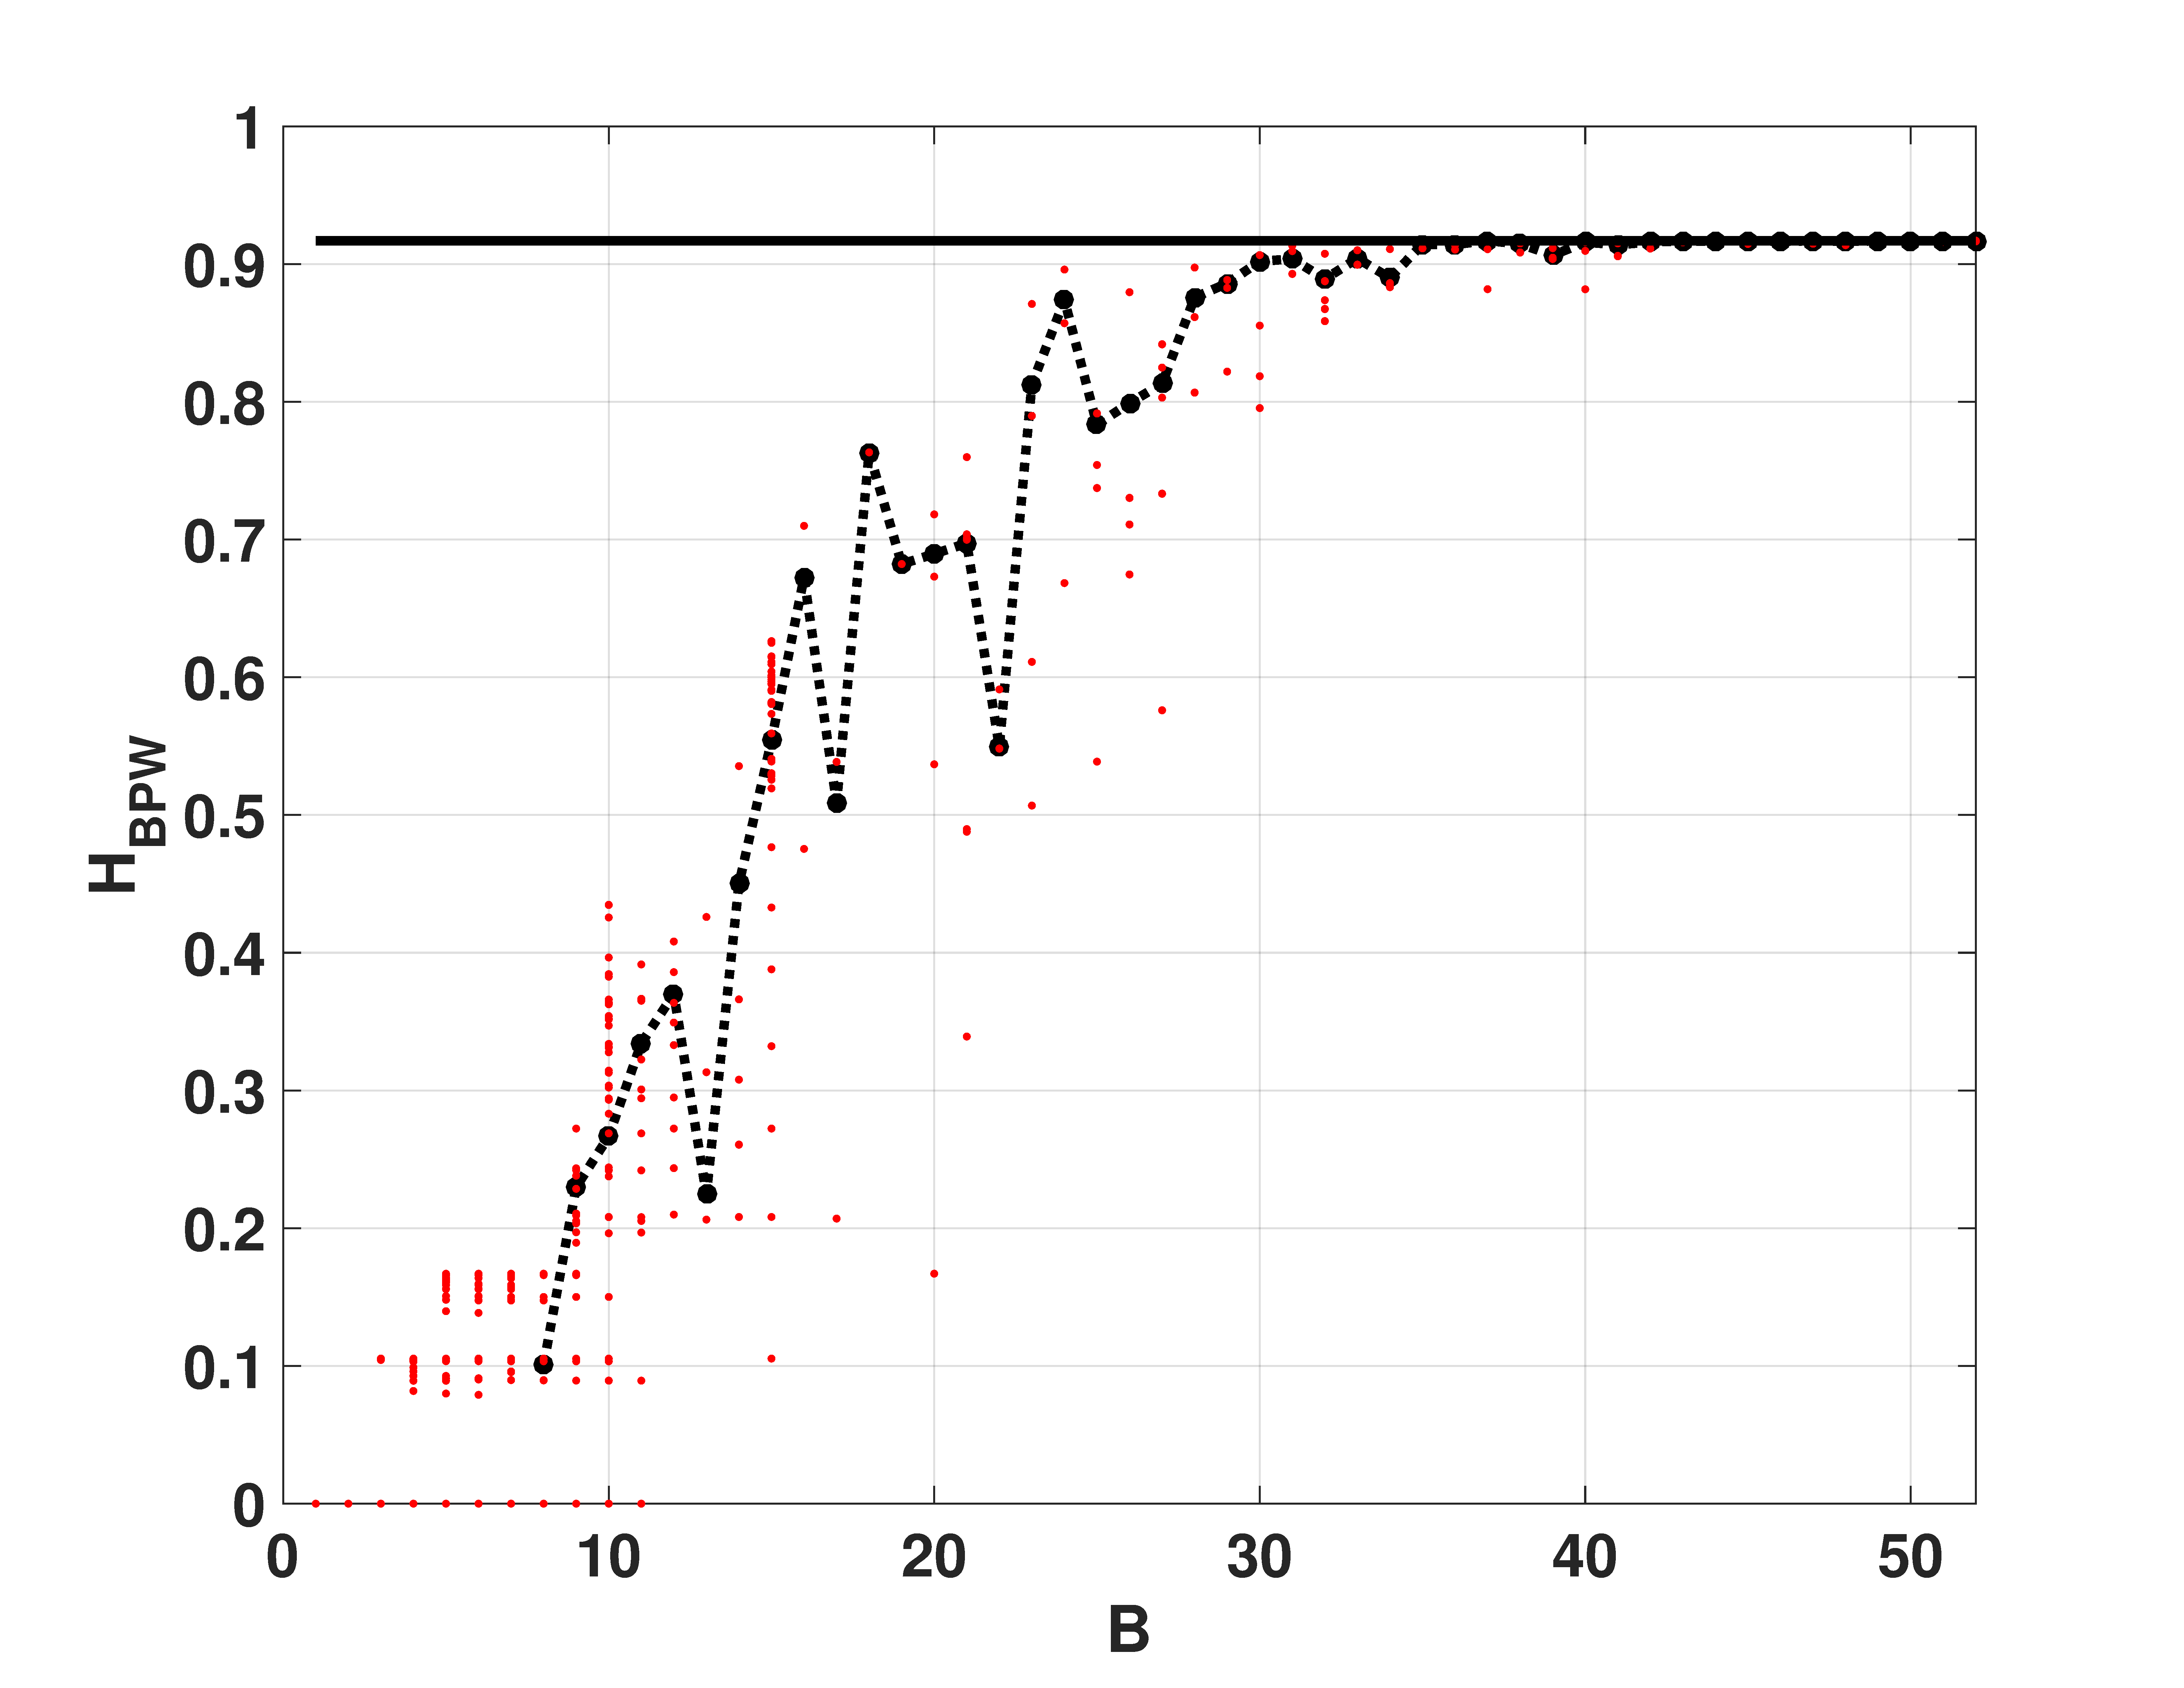
\includegraphics[width=.49\textwidth]{Hbpw_SwitchOdd}
	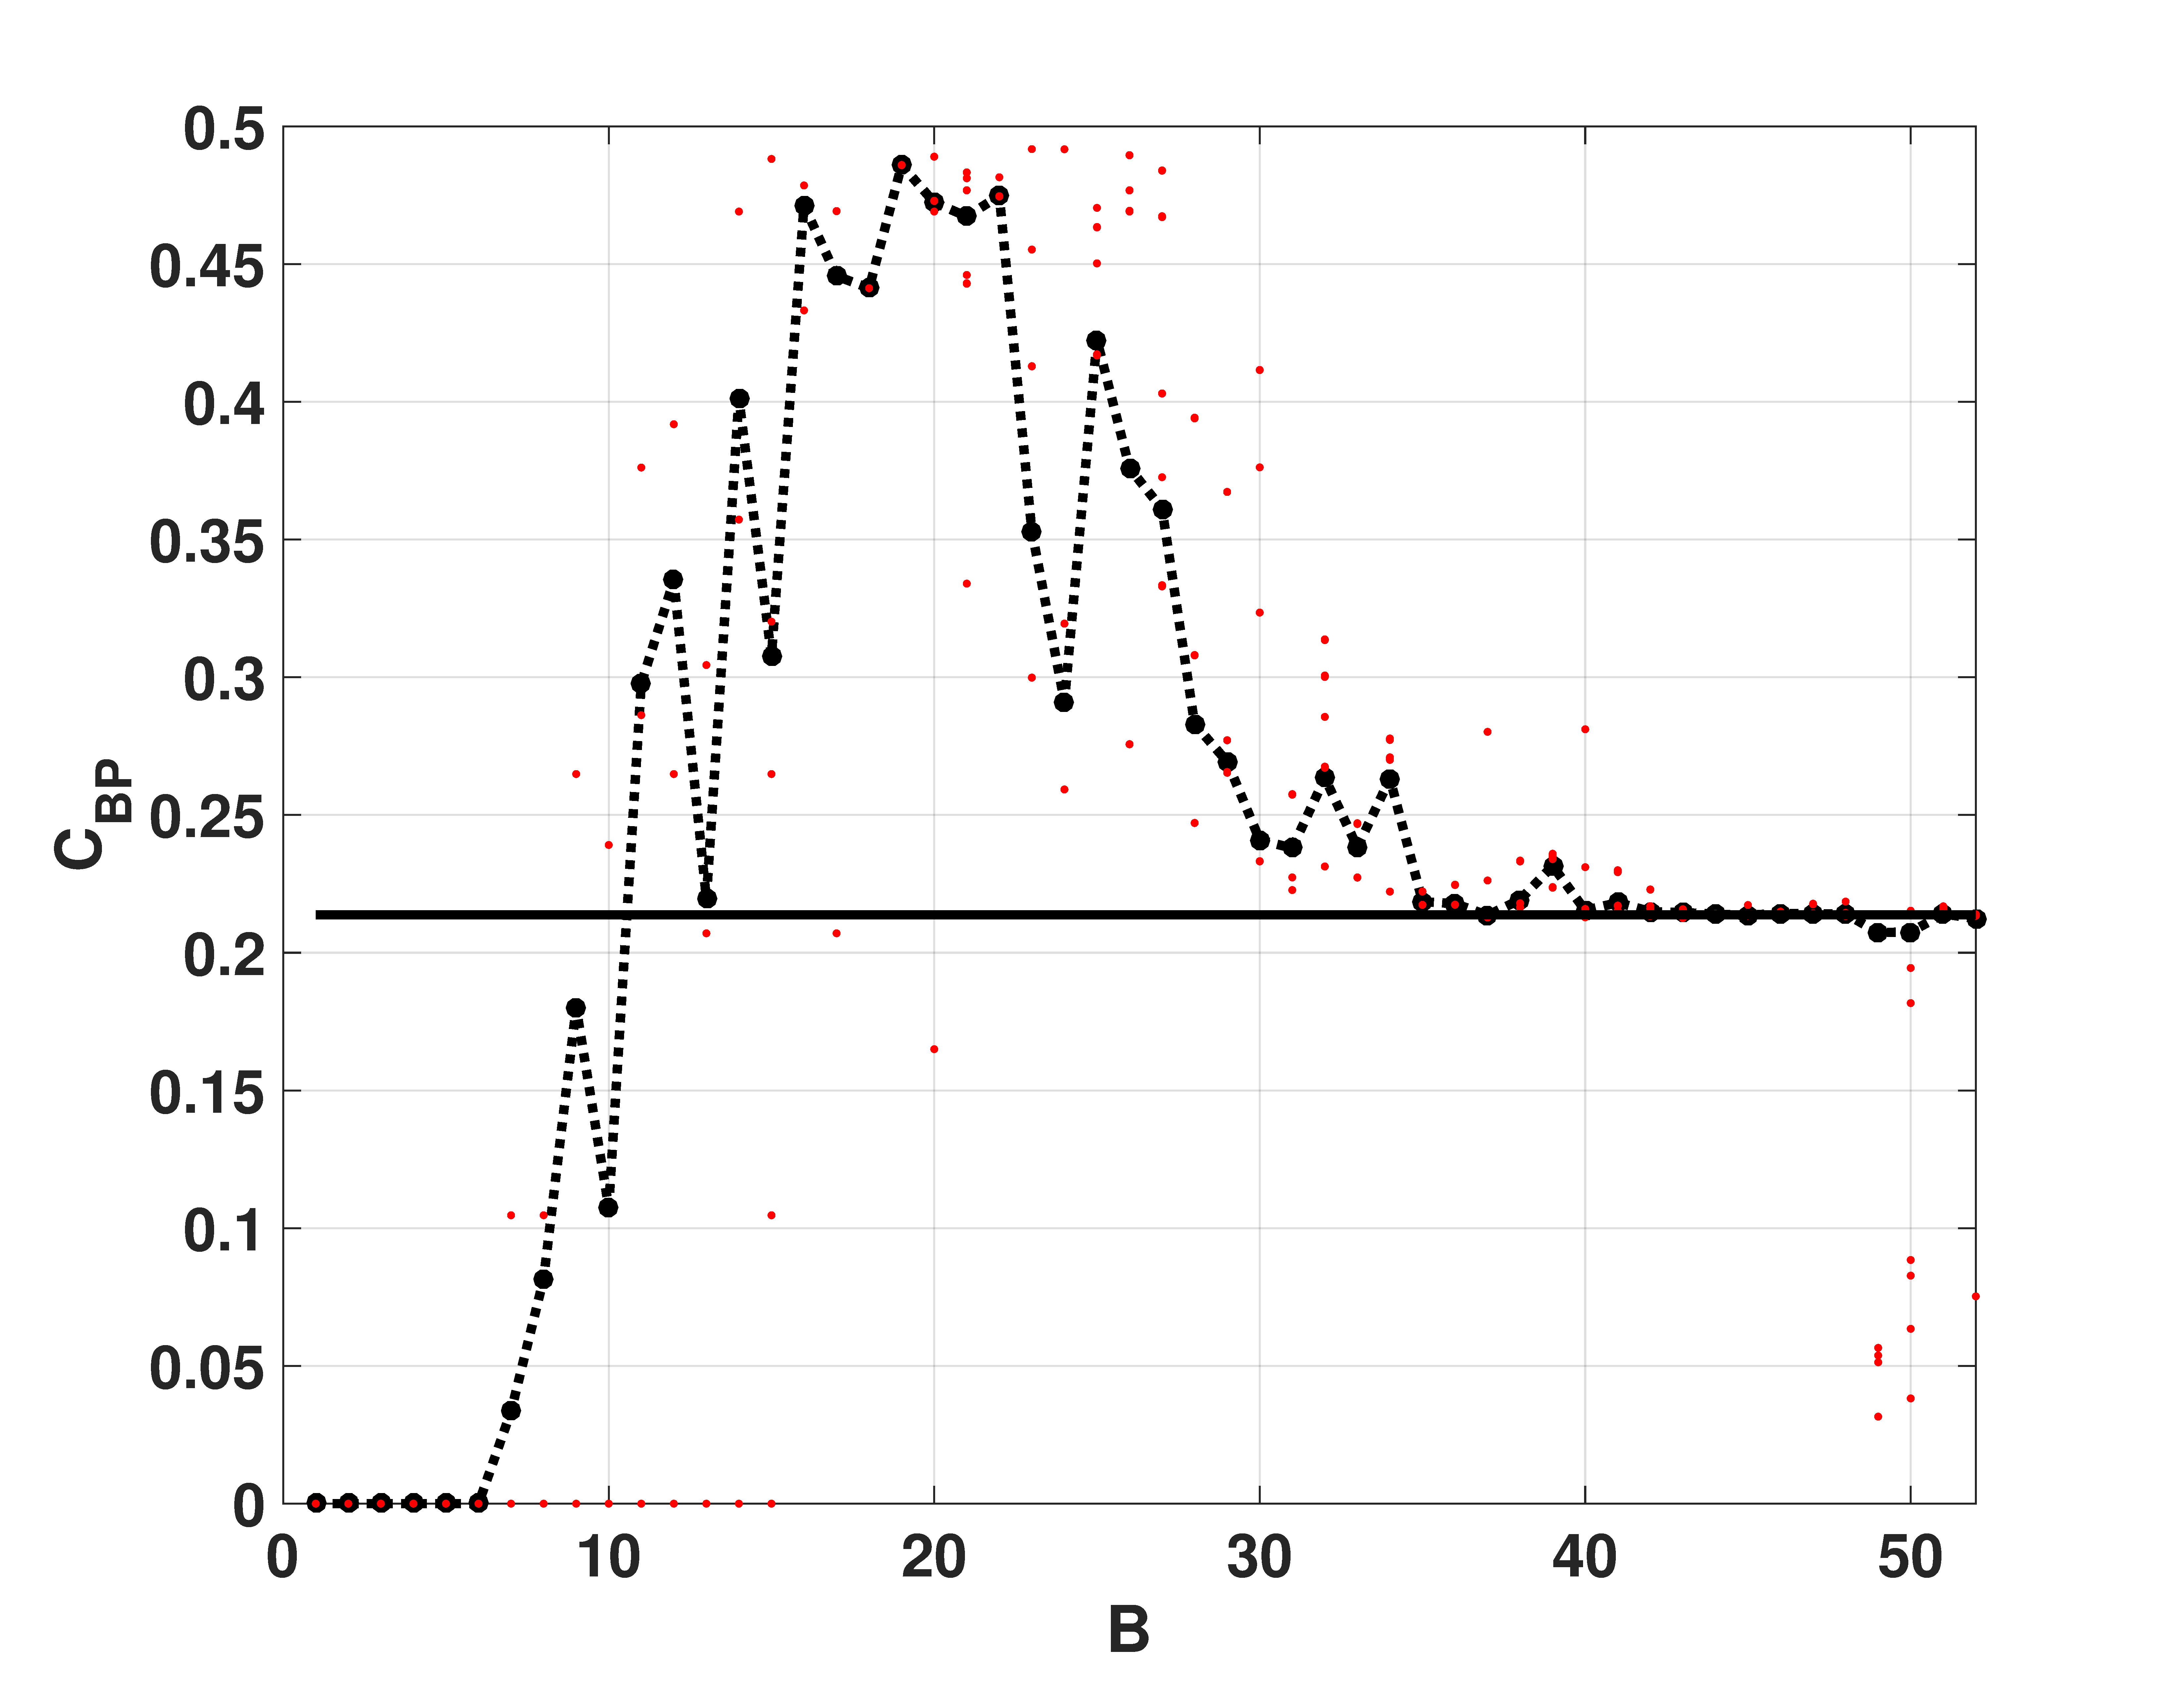
\includegraphics[width=.49\textwidth]{Cbp_SwitchOdd}
	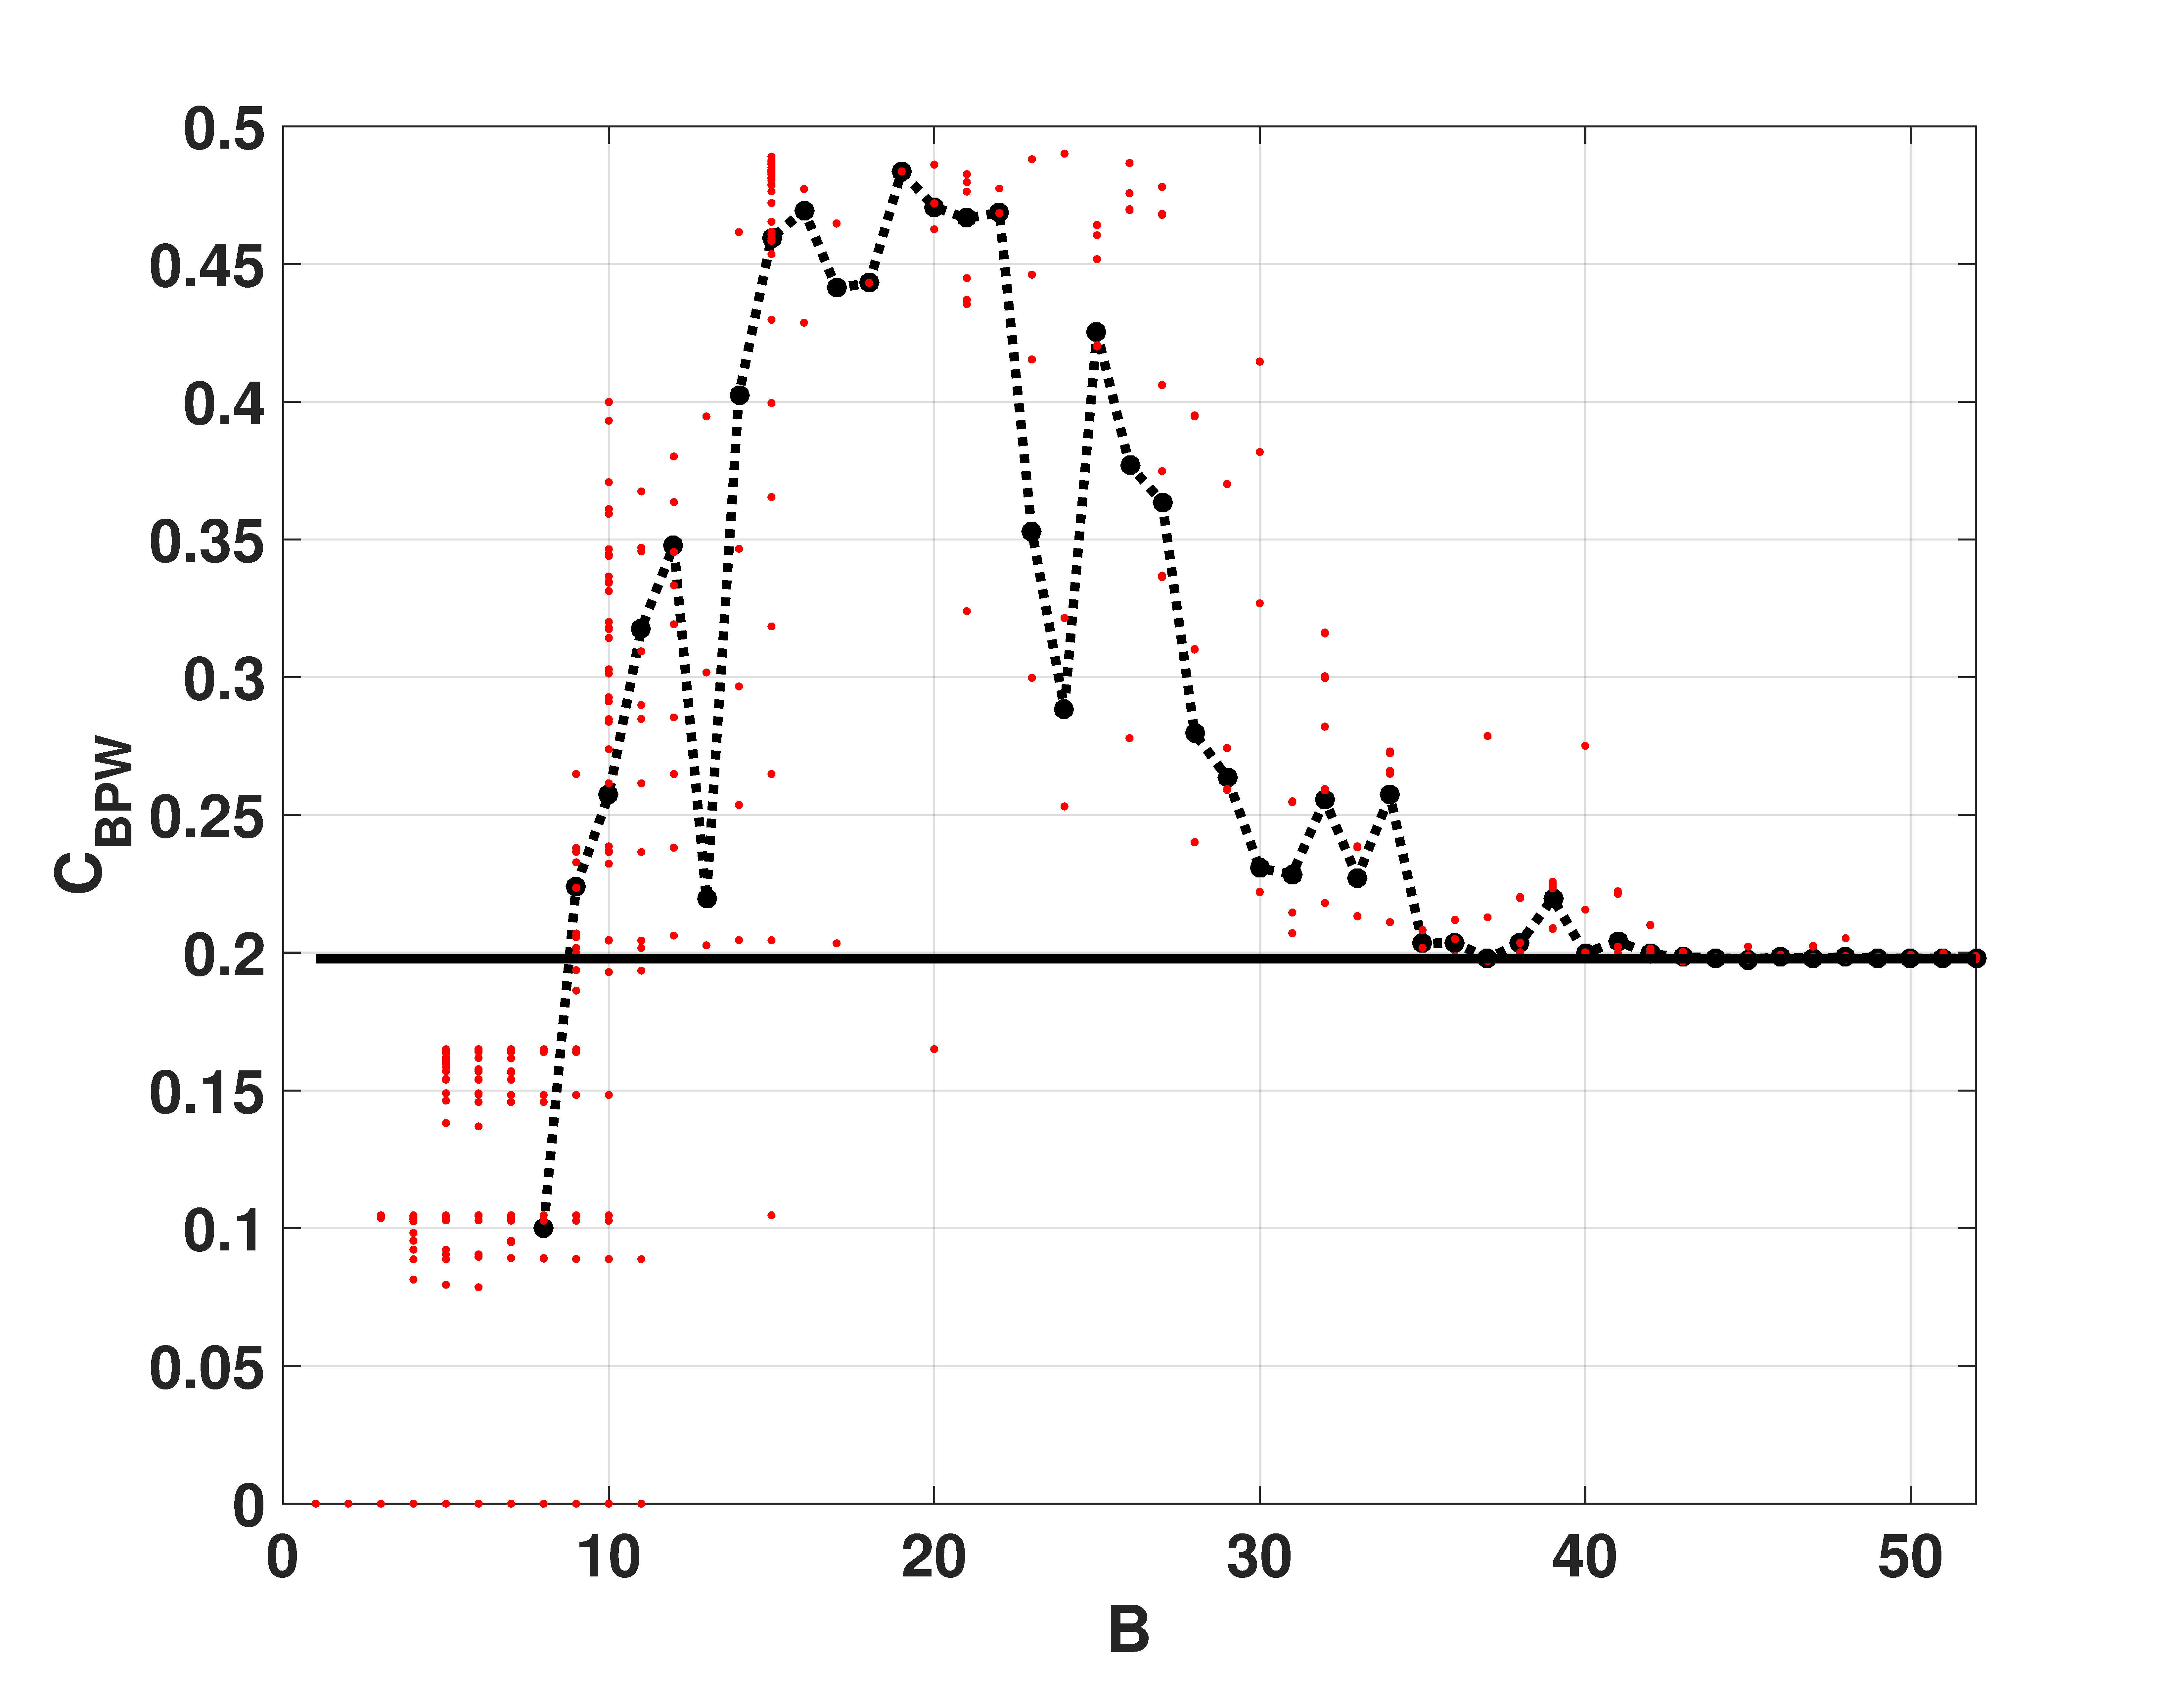
\includegraphics[width=.49\textwidth]{Cbpw_SwitchOdd}
	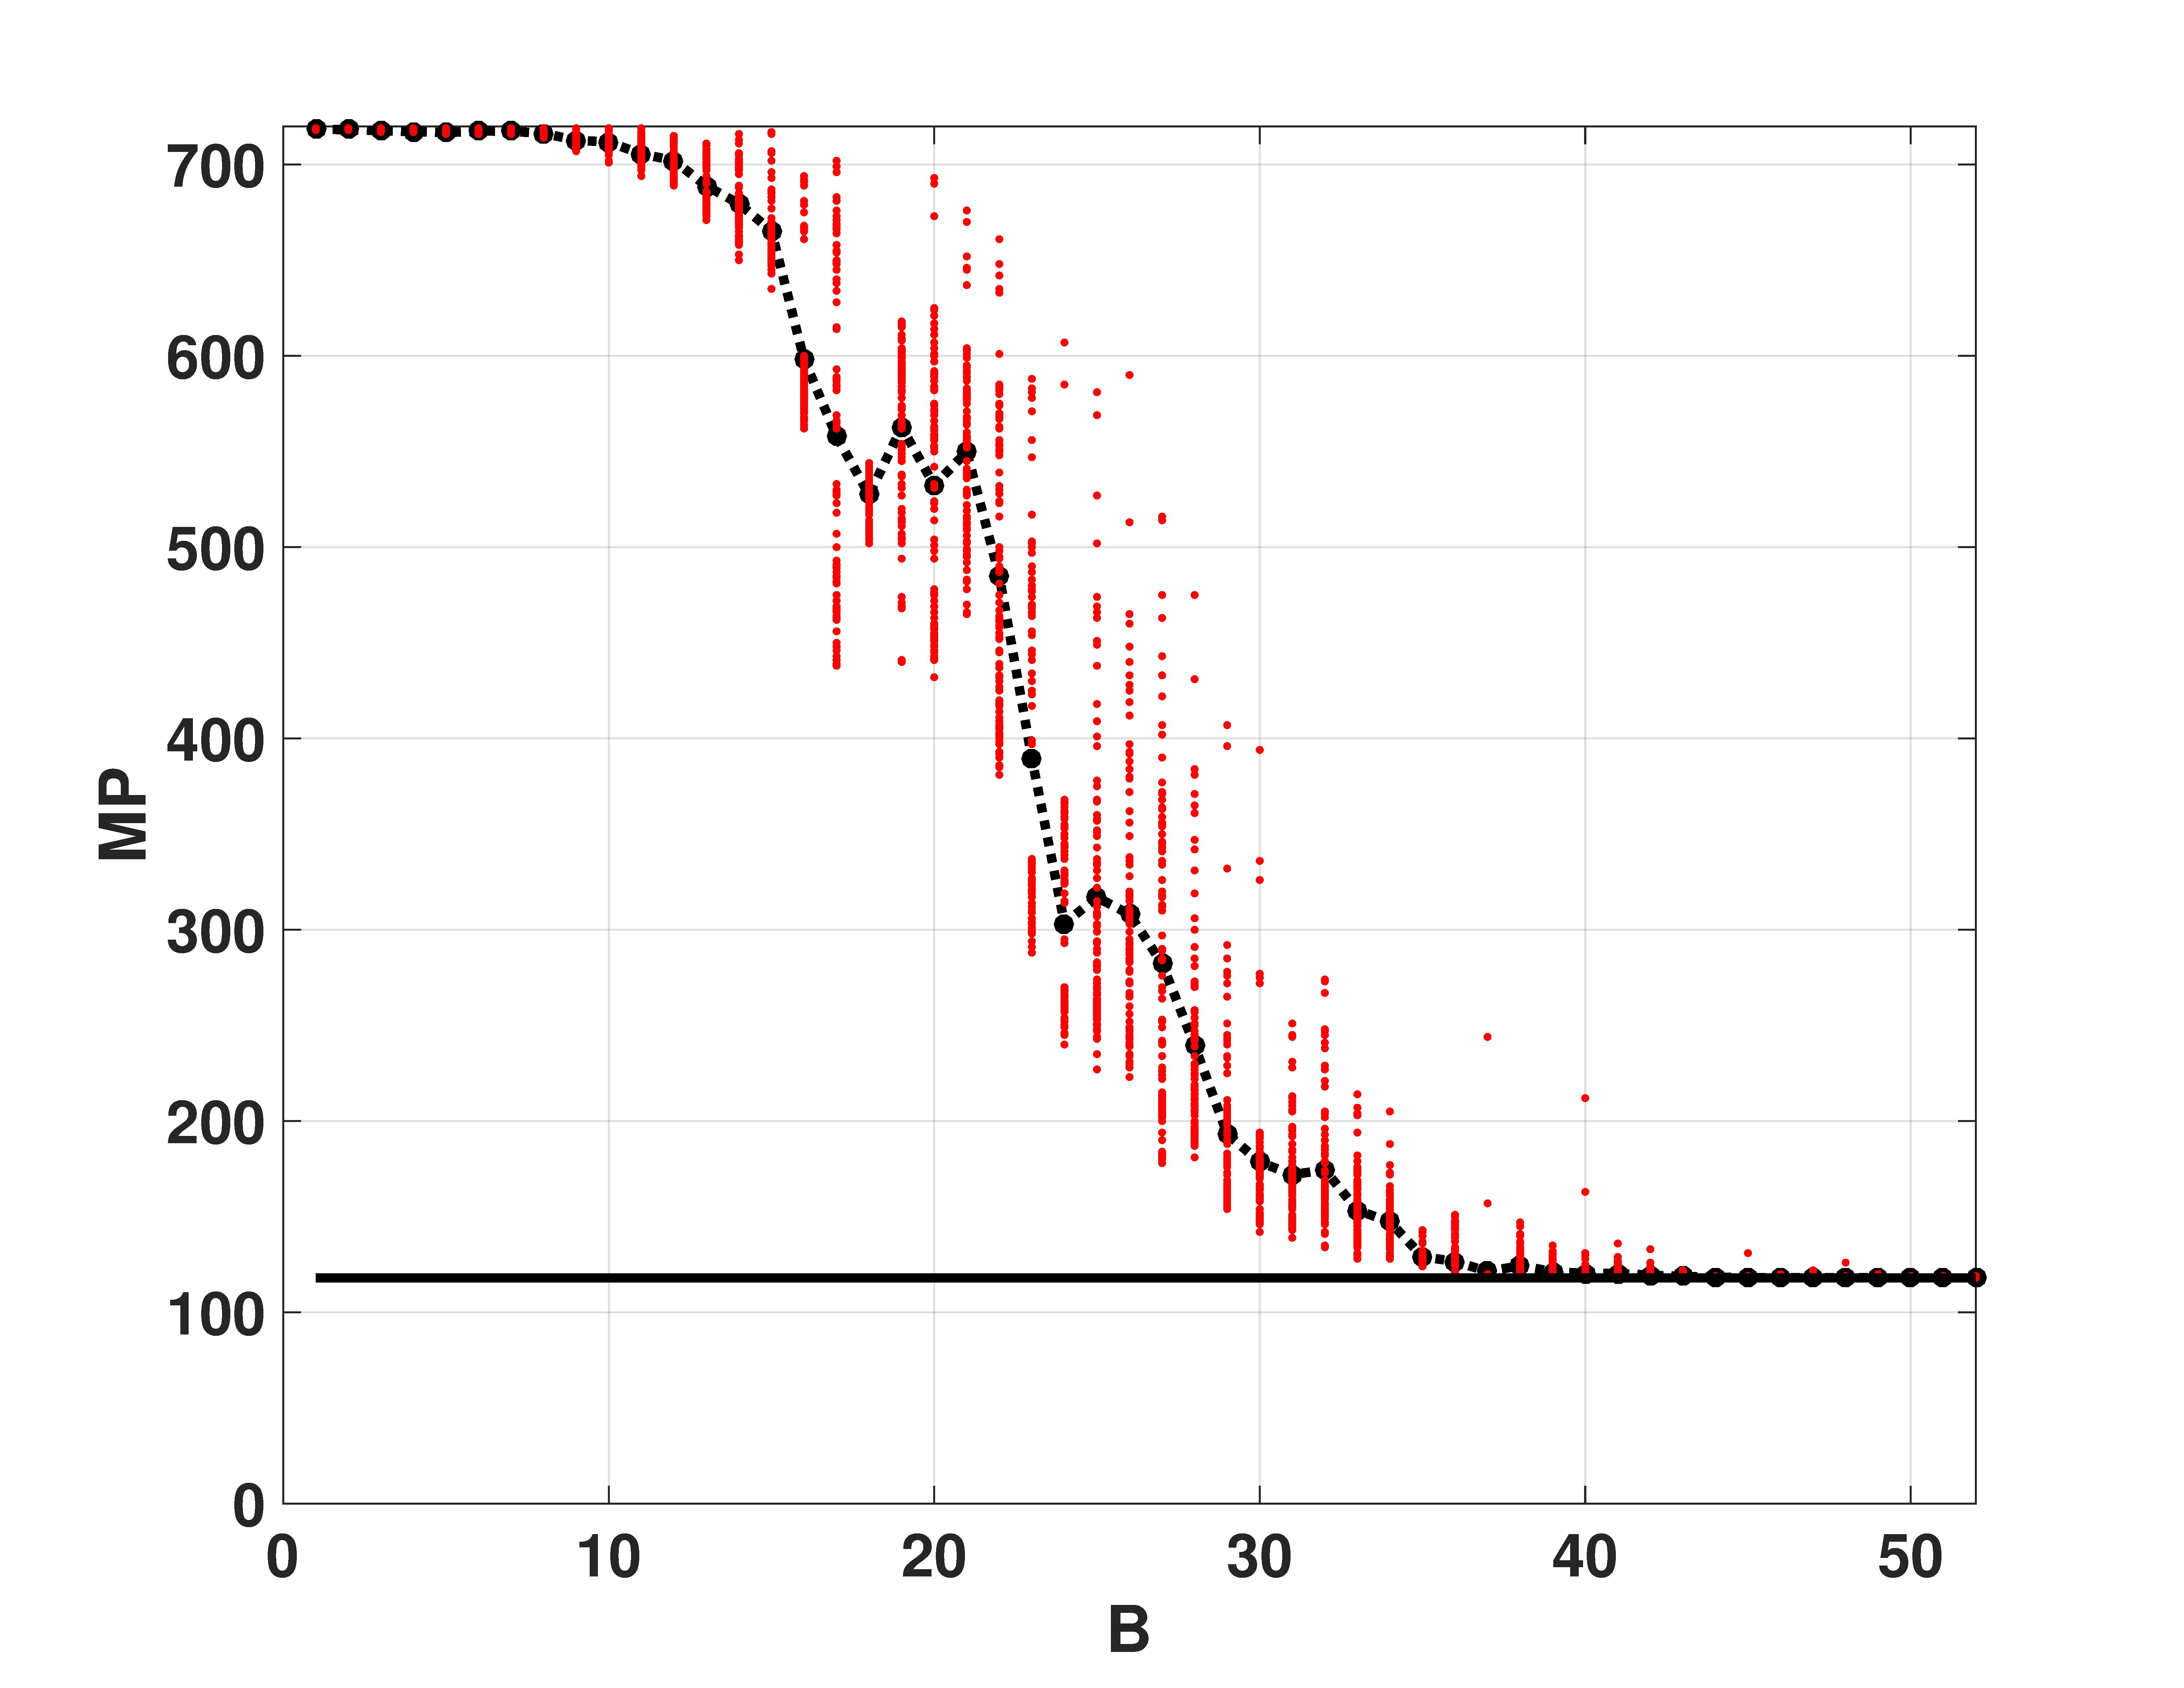
\includegraphics[width=.49\textwidth]{MP_SwitchOdd}
	\caption{Statistical properties of the LOG map using binary representation: (a) $H_{val}$ vs $B$ (b) $H_{BP}$ vs $B$ (c) $C_{BP}$ vs $B$ (d) Number of missing ordering patterns $MP$ vs $B$.}
	\label{fig:ODD_QuantiB}
	\end{figure}

\textcolor{red}{PLANOS DOBLE ENTROPÍA}

\begin{figure}
	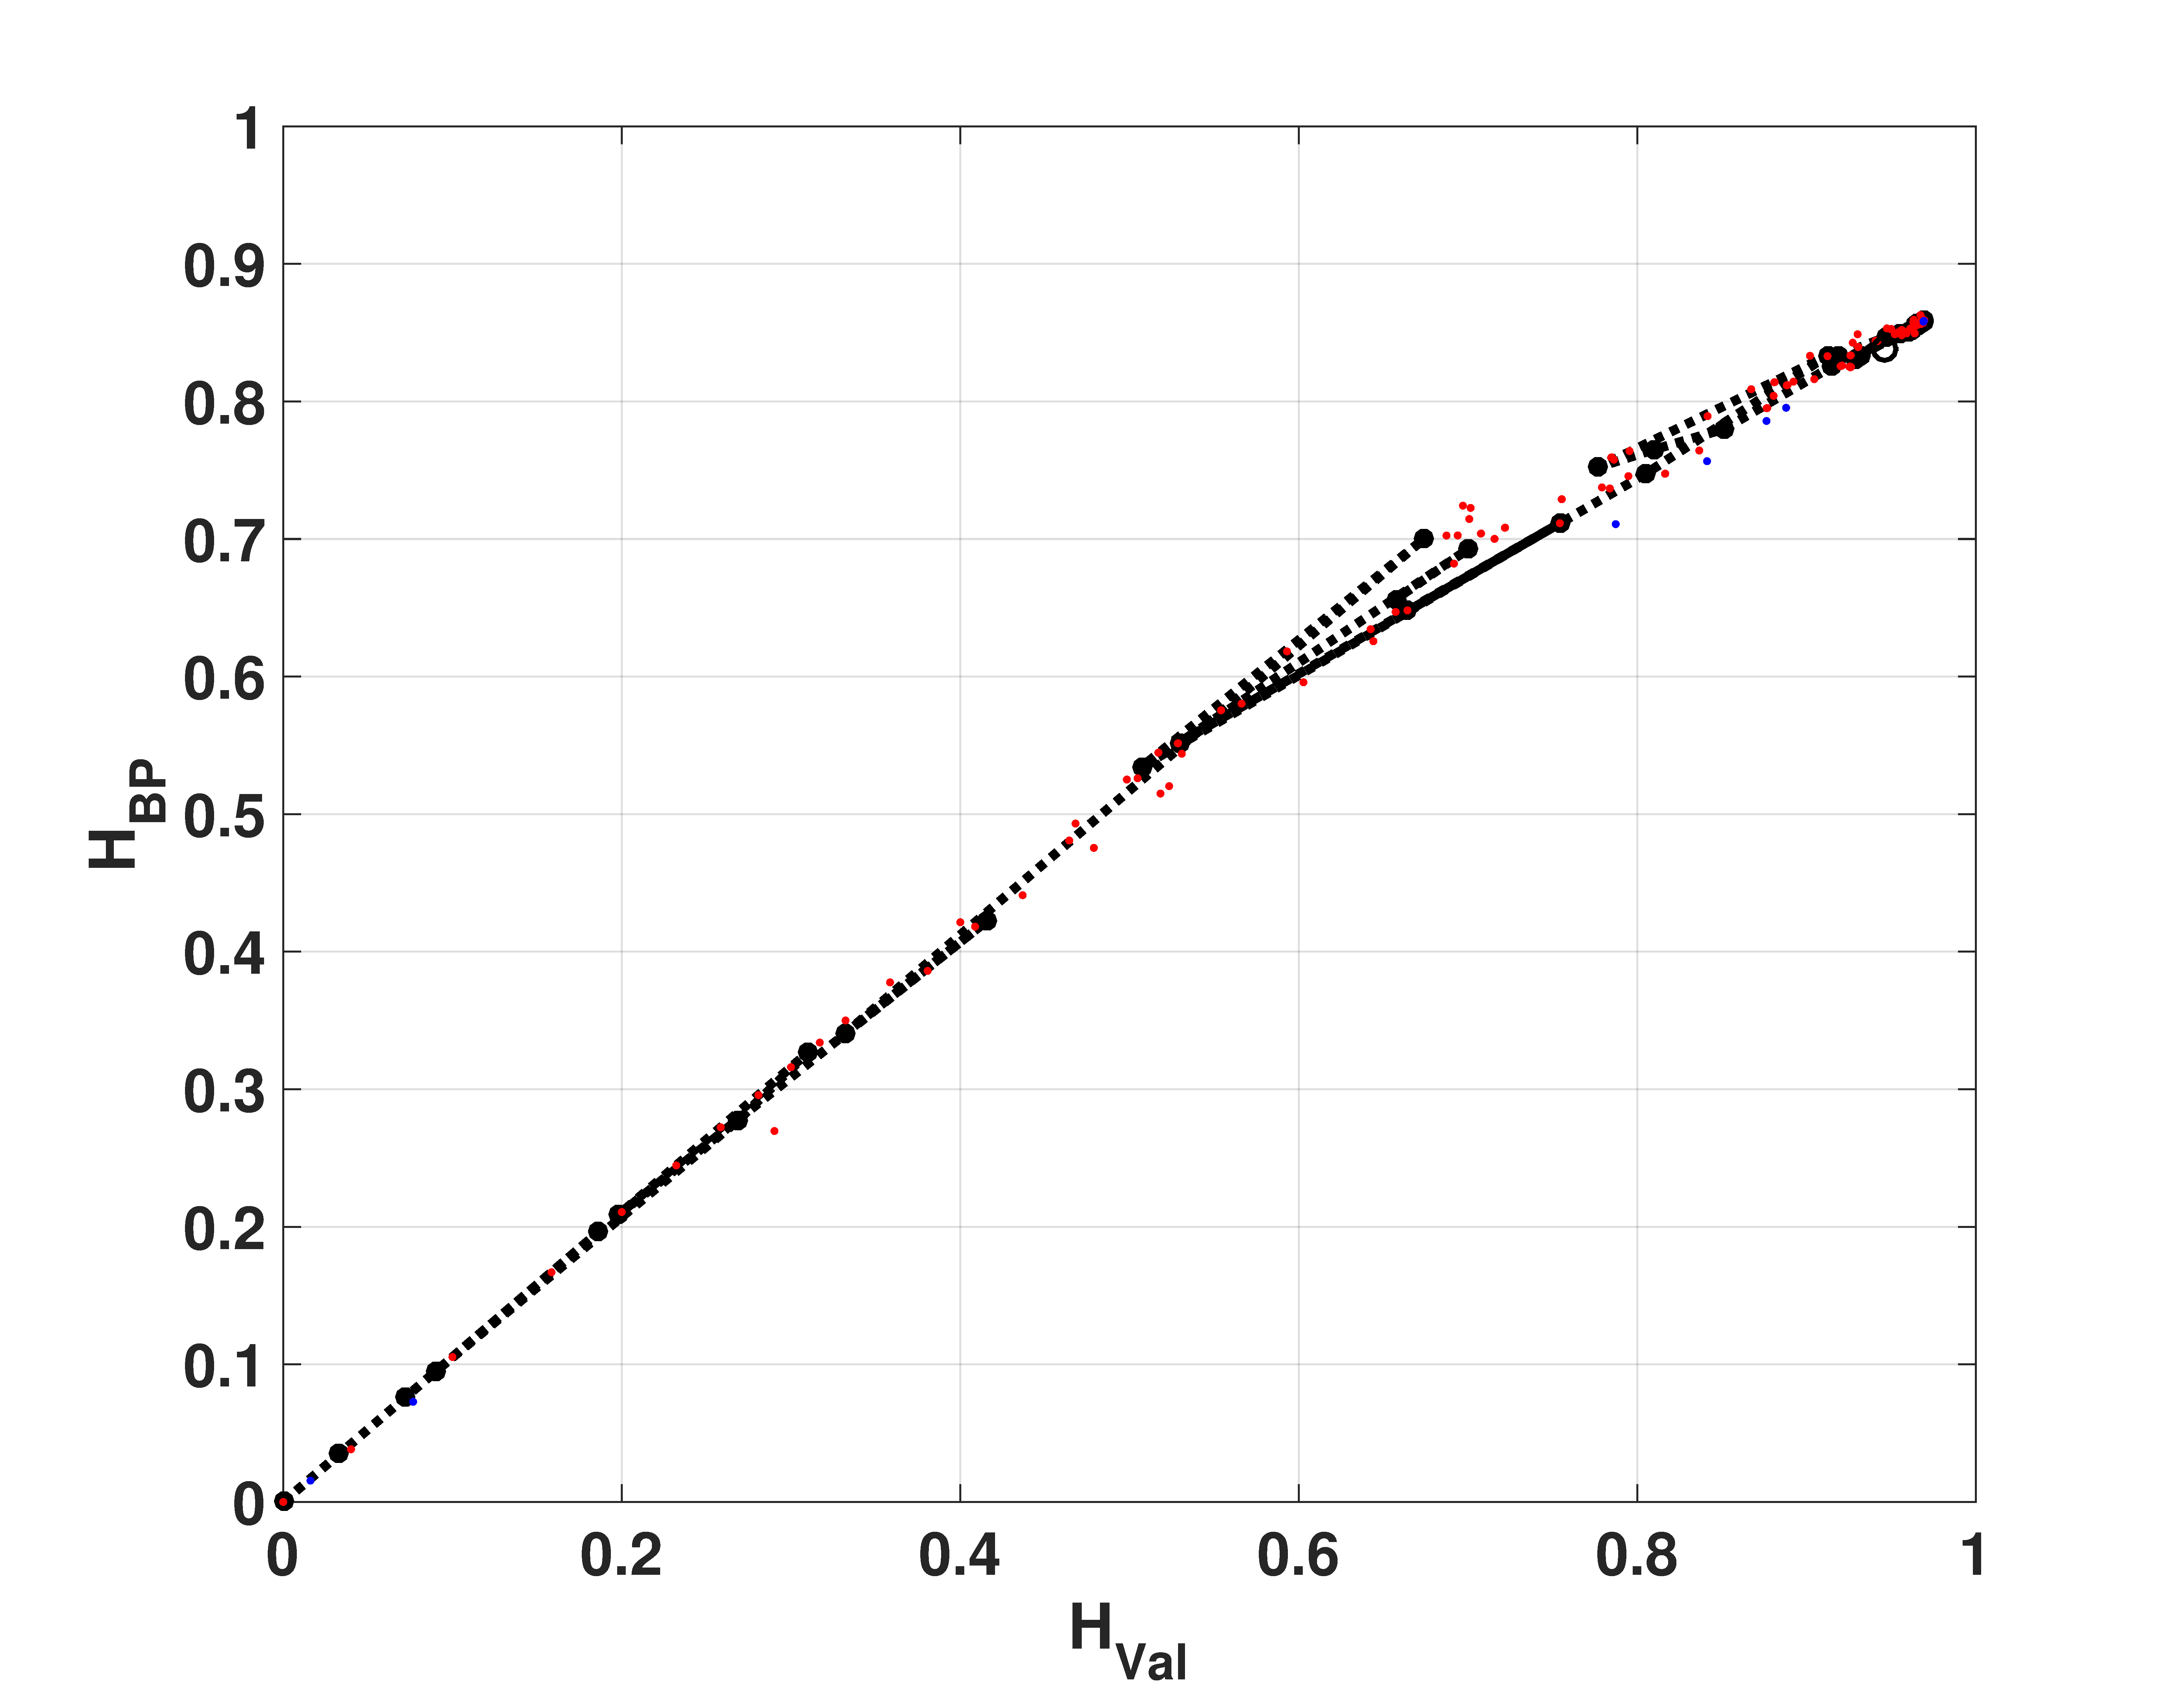
\includegraphics[width=.49\textwidth]{HbpHval_SwitchEven}
	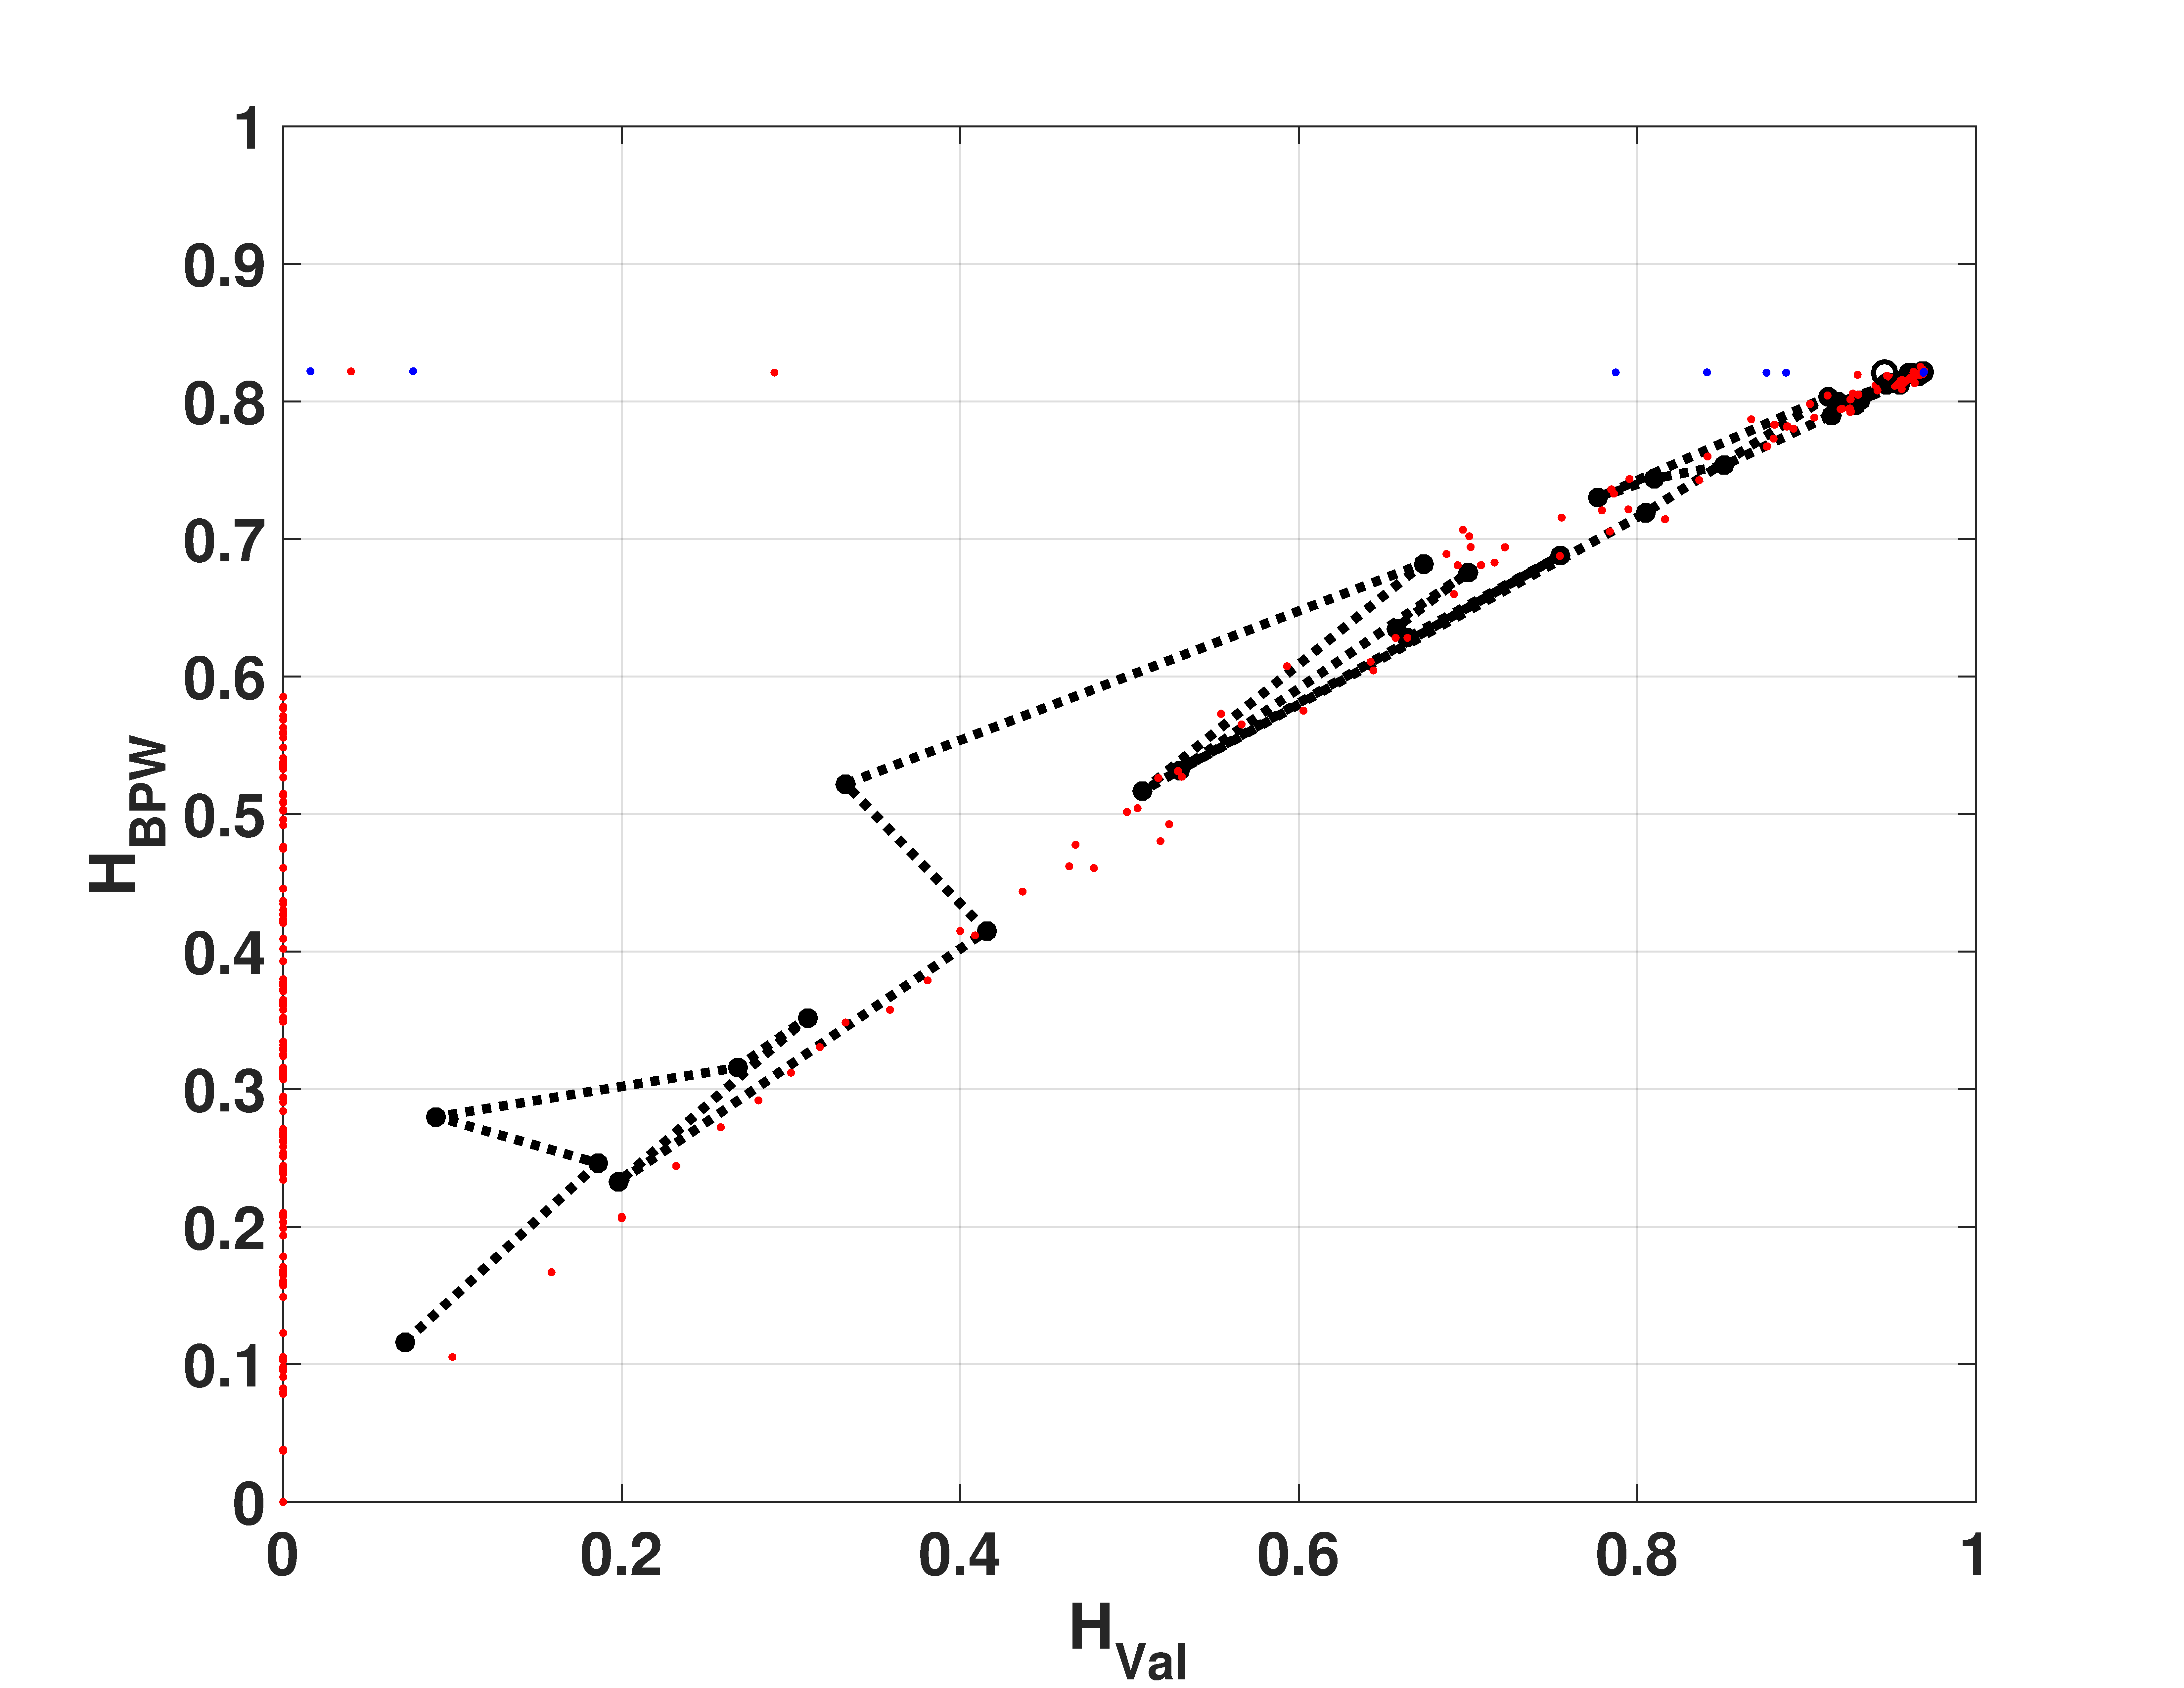
\includegraphics[width=.49\textwidth]{HbpwHval_SwitchEven}
	\caption{Evolution of statistical properties in double entropy plane of LOG map using binary representation: (a) $H_{val}$ vs $H_{BP}$ (b) $H_{val}$ vs $H_{BPW}$.}
	\label{fig:EVEN_HH}
\end{figure}

\begin{figure}
	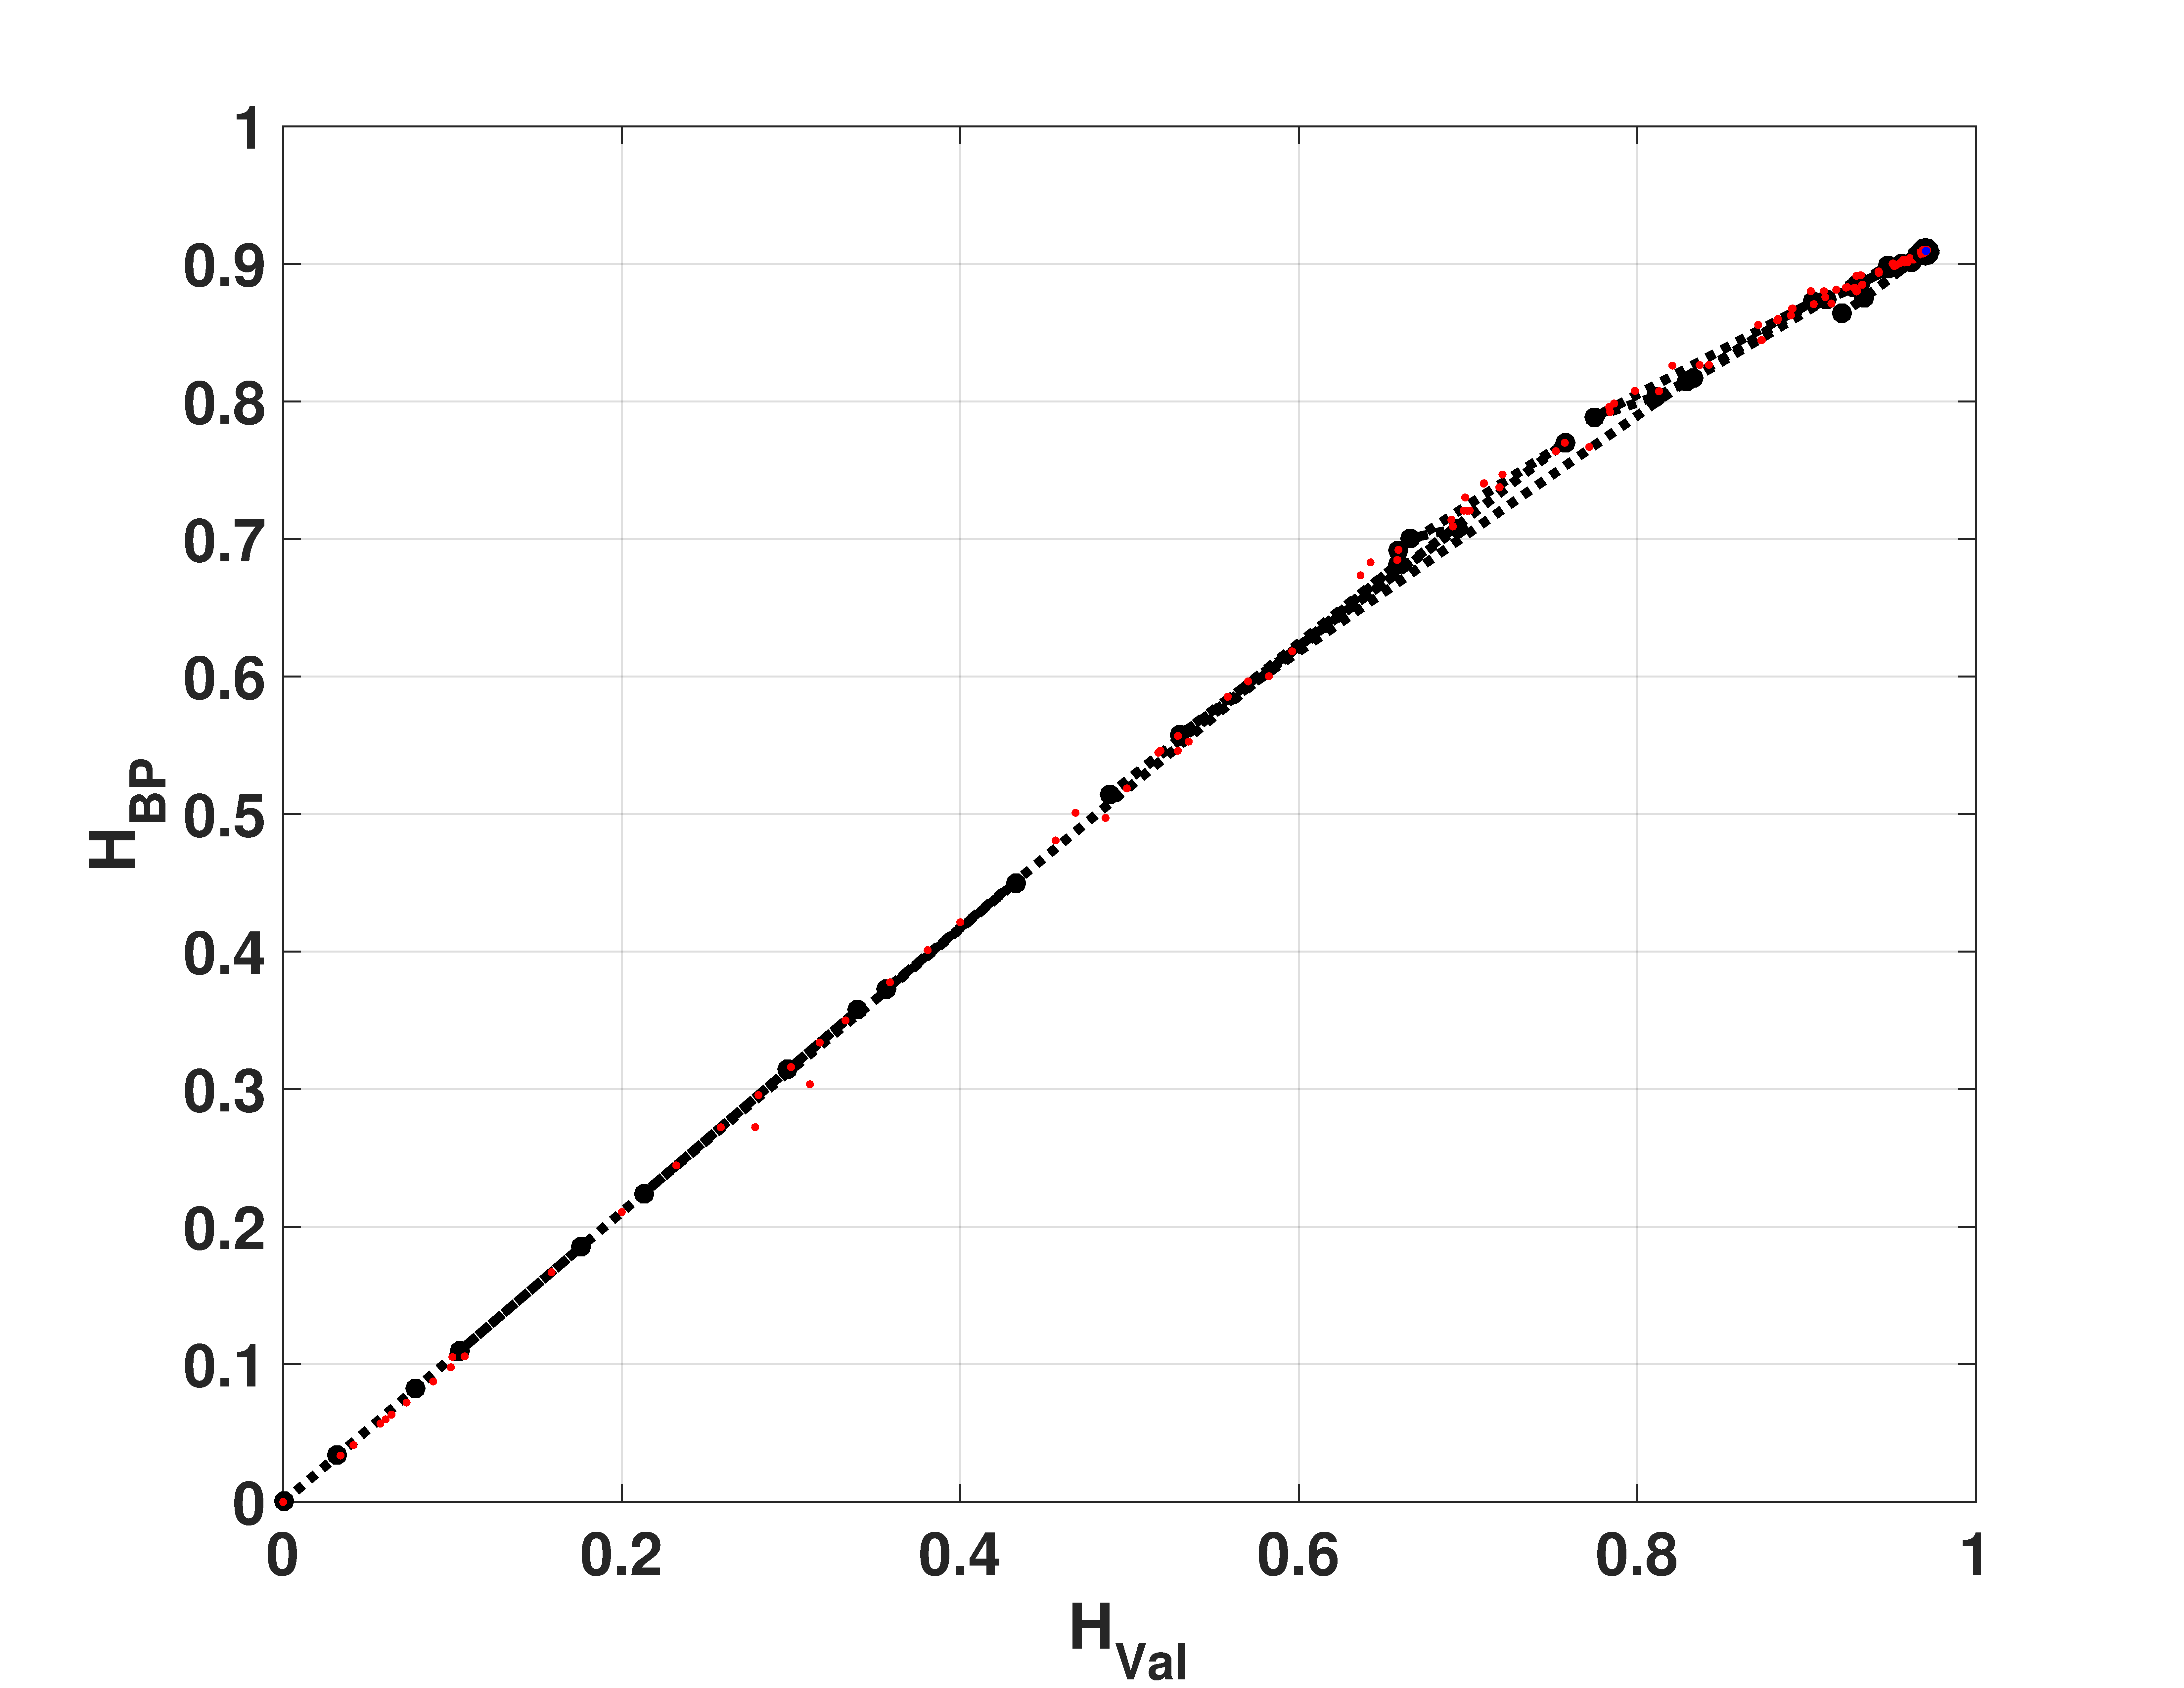
\includegraphics[width=.49\textwidth]{HbpHval_SwitchOdd}
	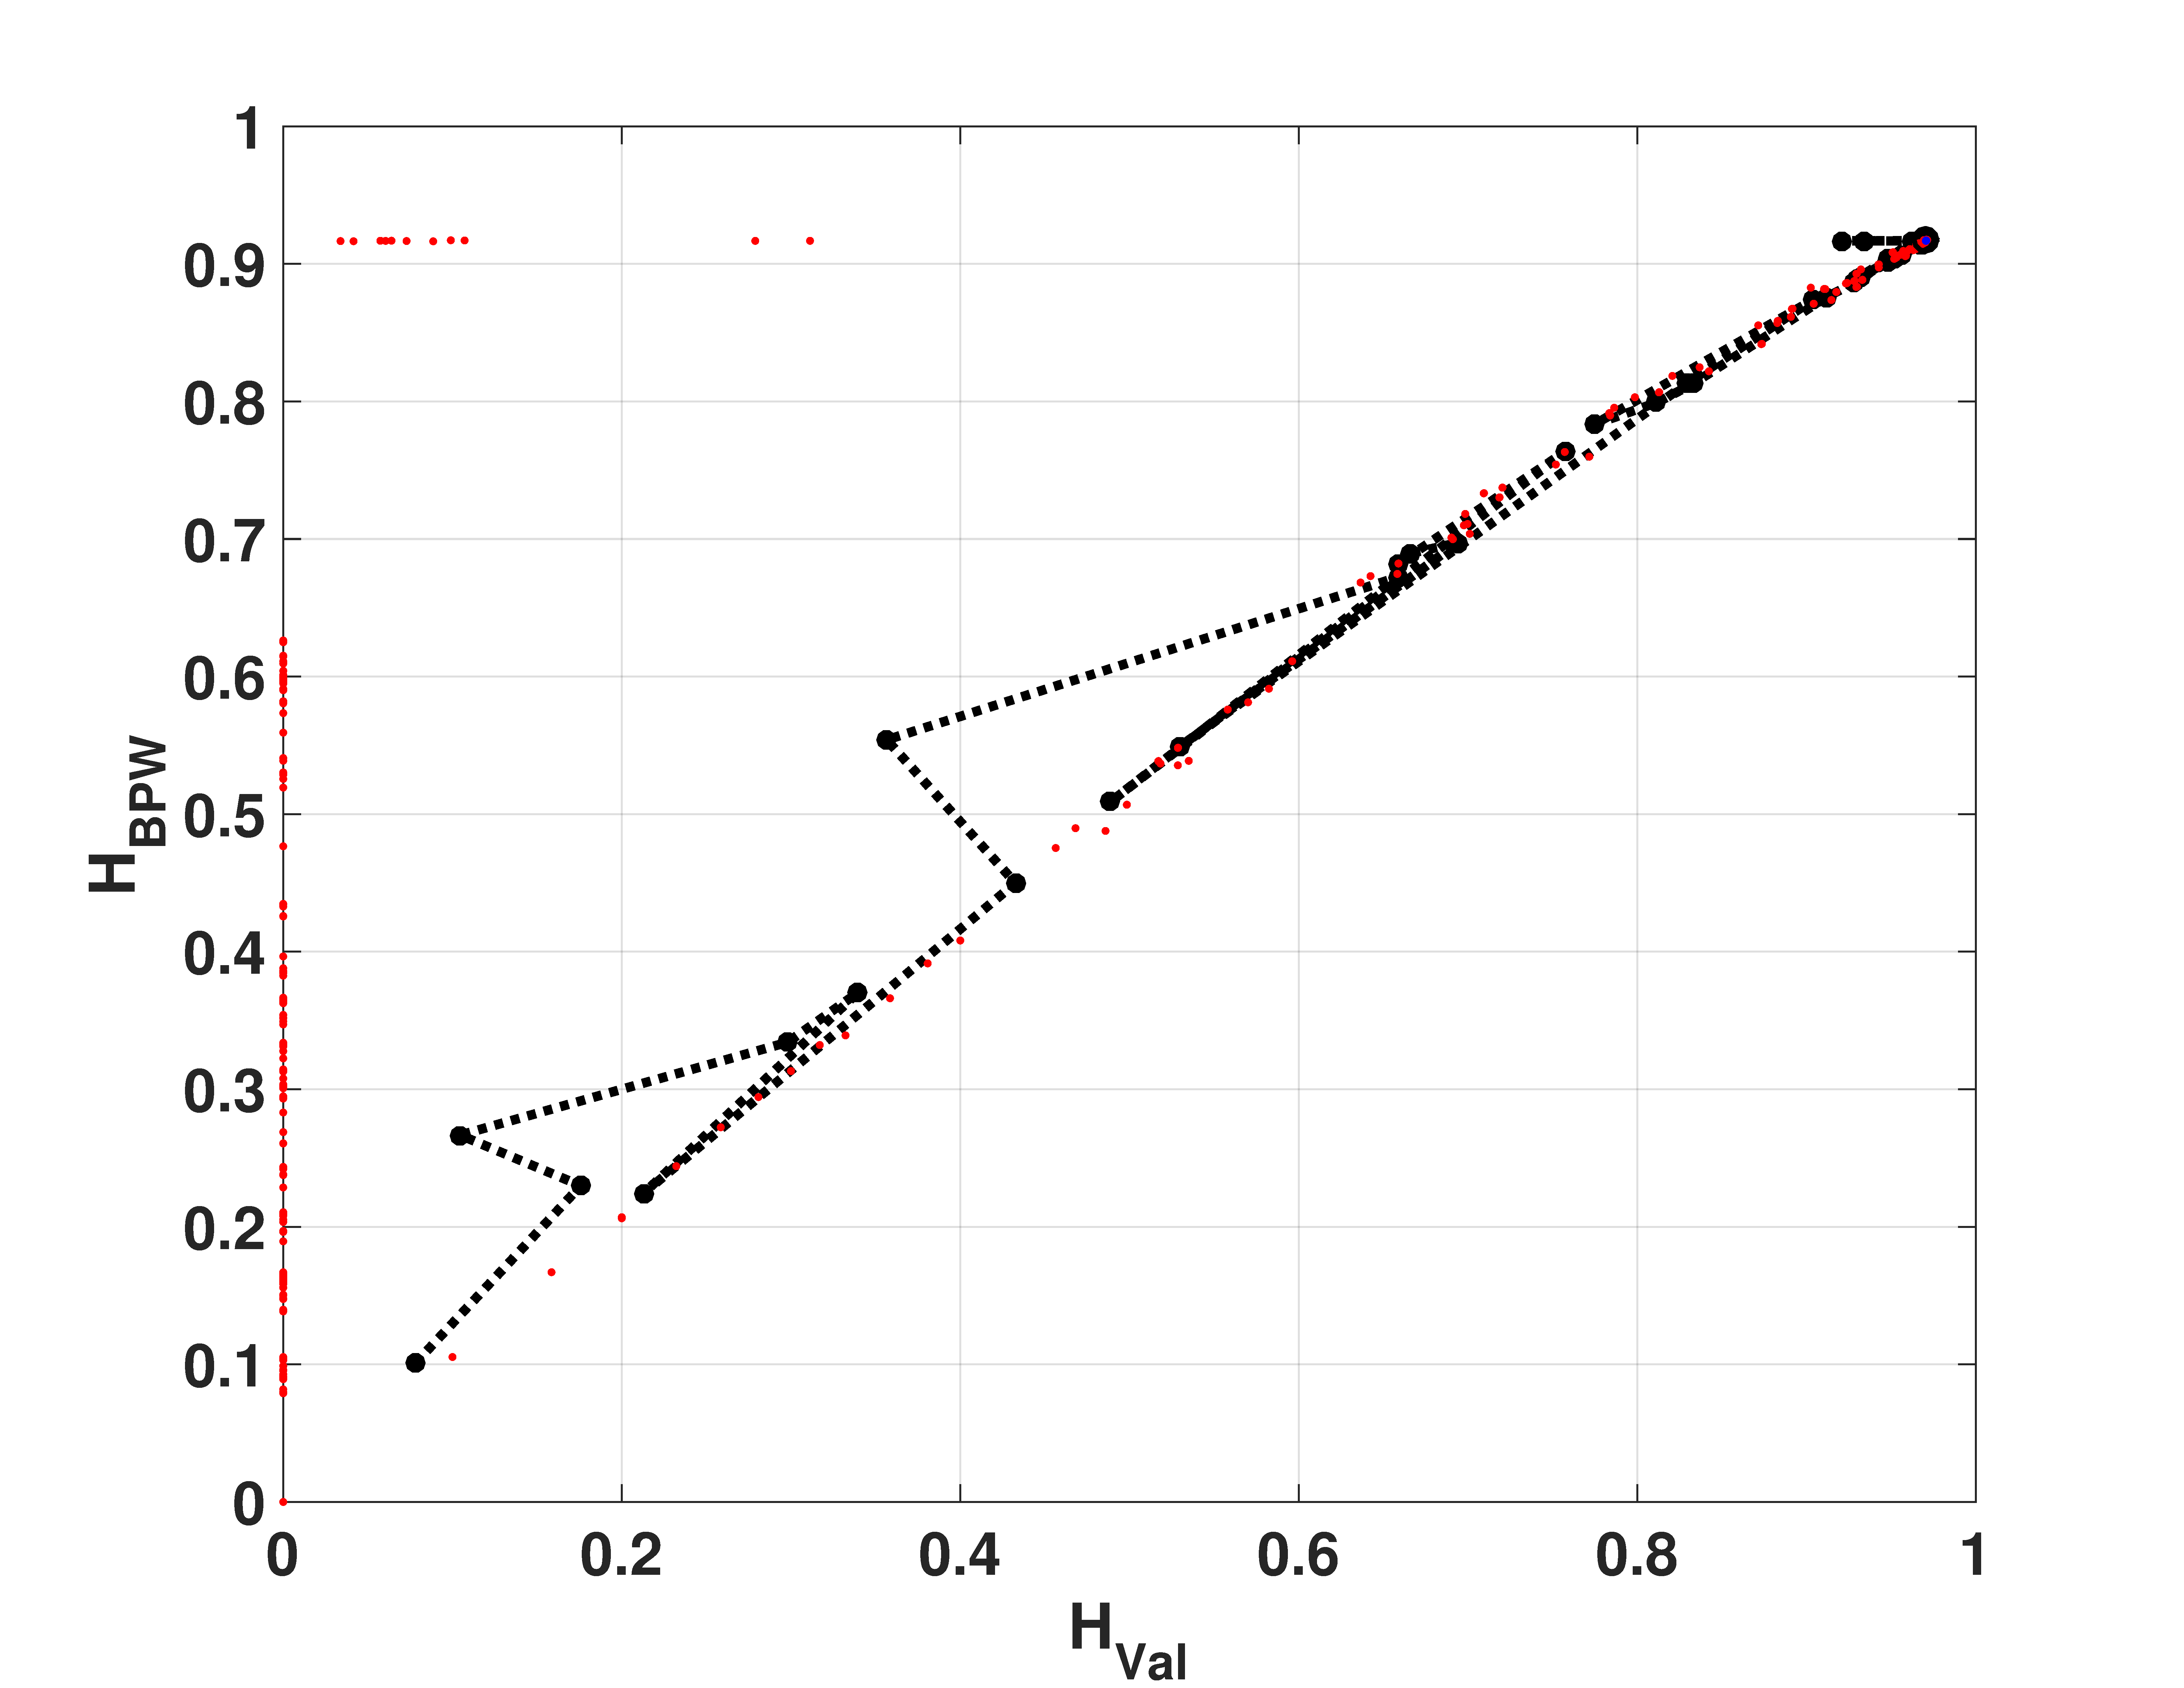
\includegraphics[width=.49\textwidth]{HbpwHval_SwitchOdd}
	\caption{Evolution of statistical properties in double entropy plane of LOG map using binary representation: (a) $H_{val}$ vs $H_{BP}$ (b) $H_{val}$ vs $H_{BPW}$.}
	\label{fig:ODD_HH}
\end{figure}

\textcolor{red}{PLANOS ENTROPÍA-COMPLEJIDAD}

\begin{figure}
	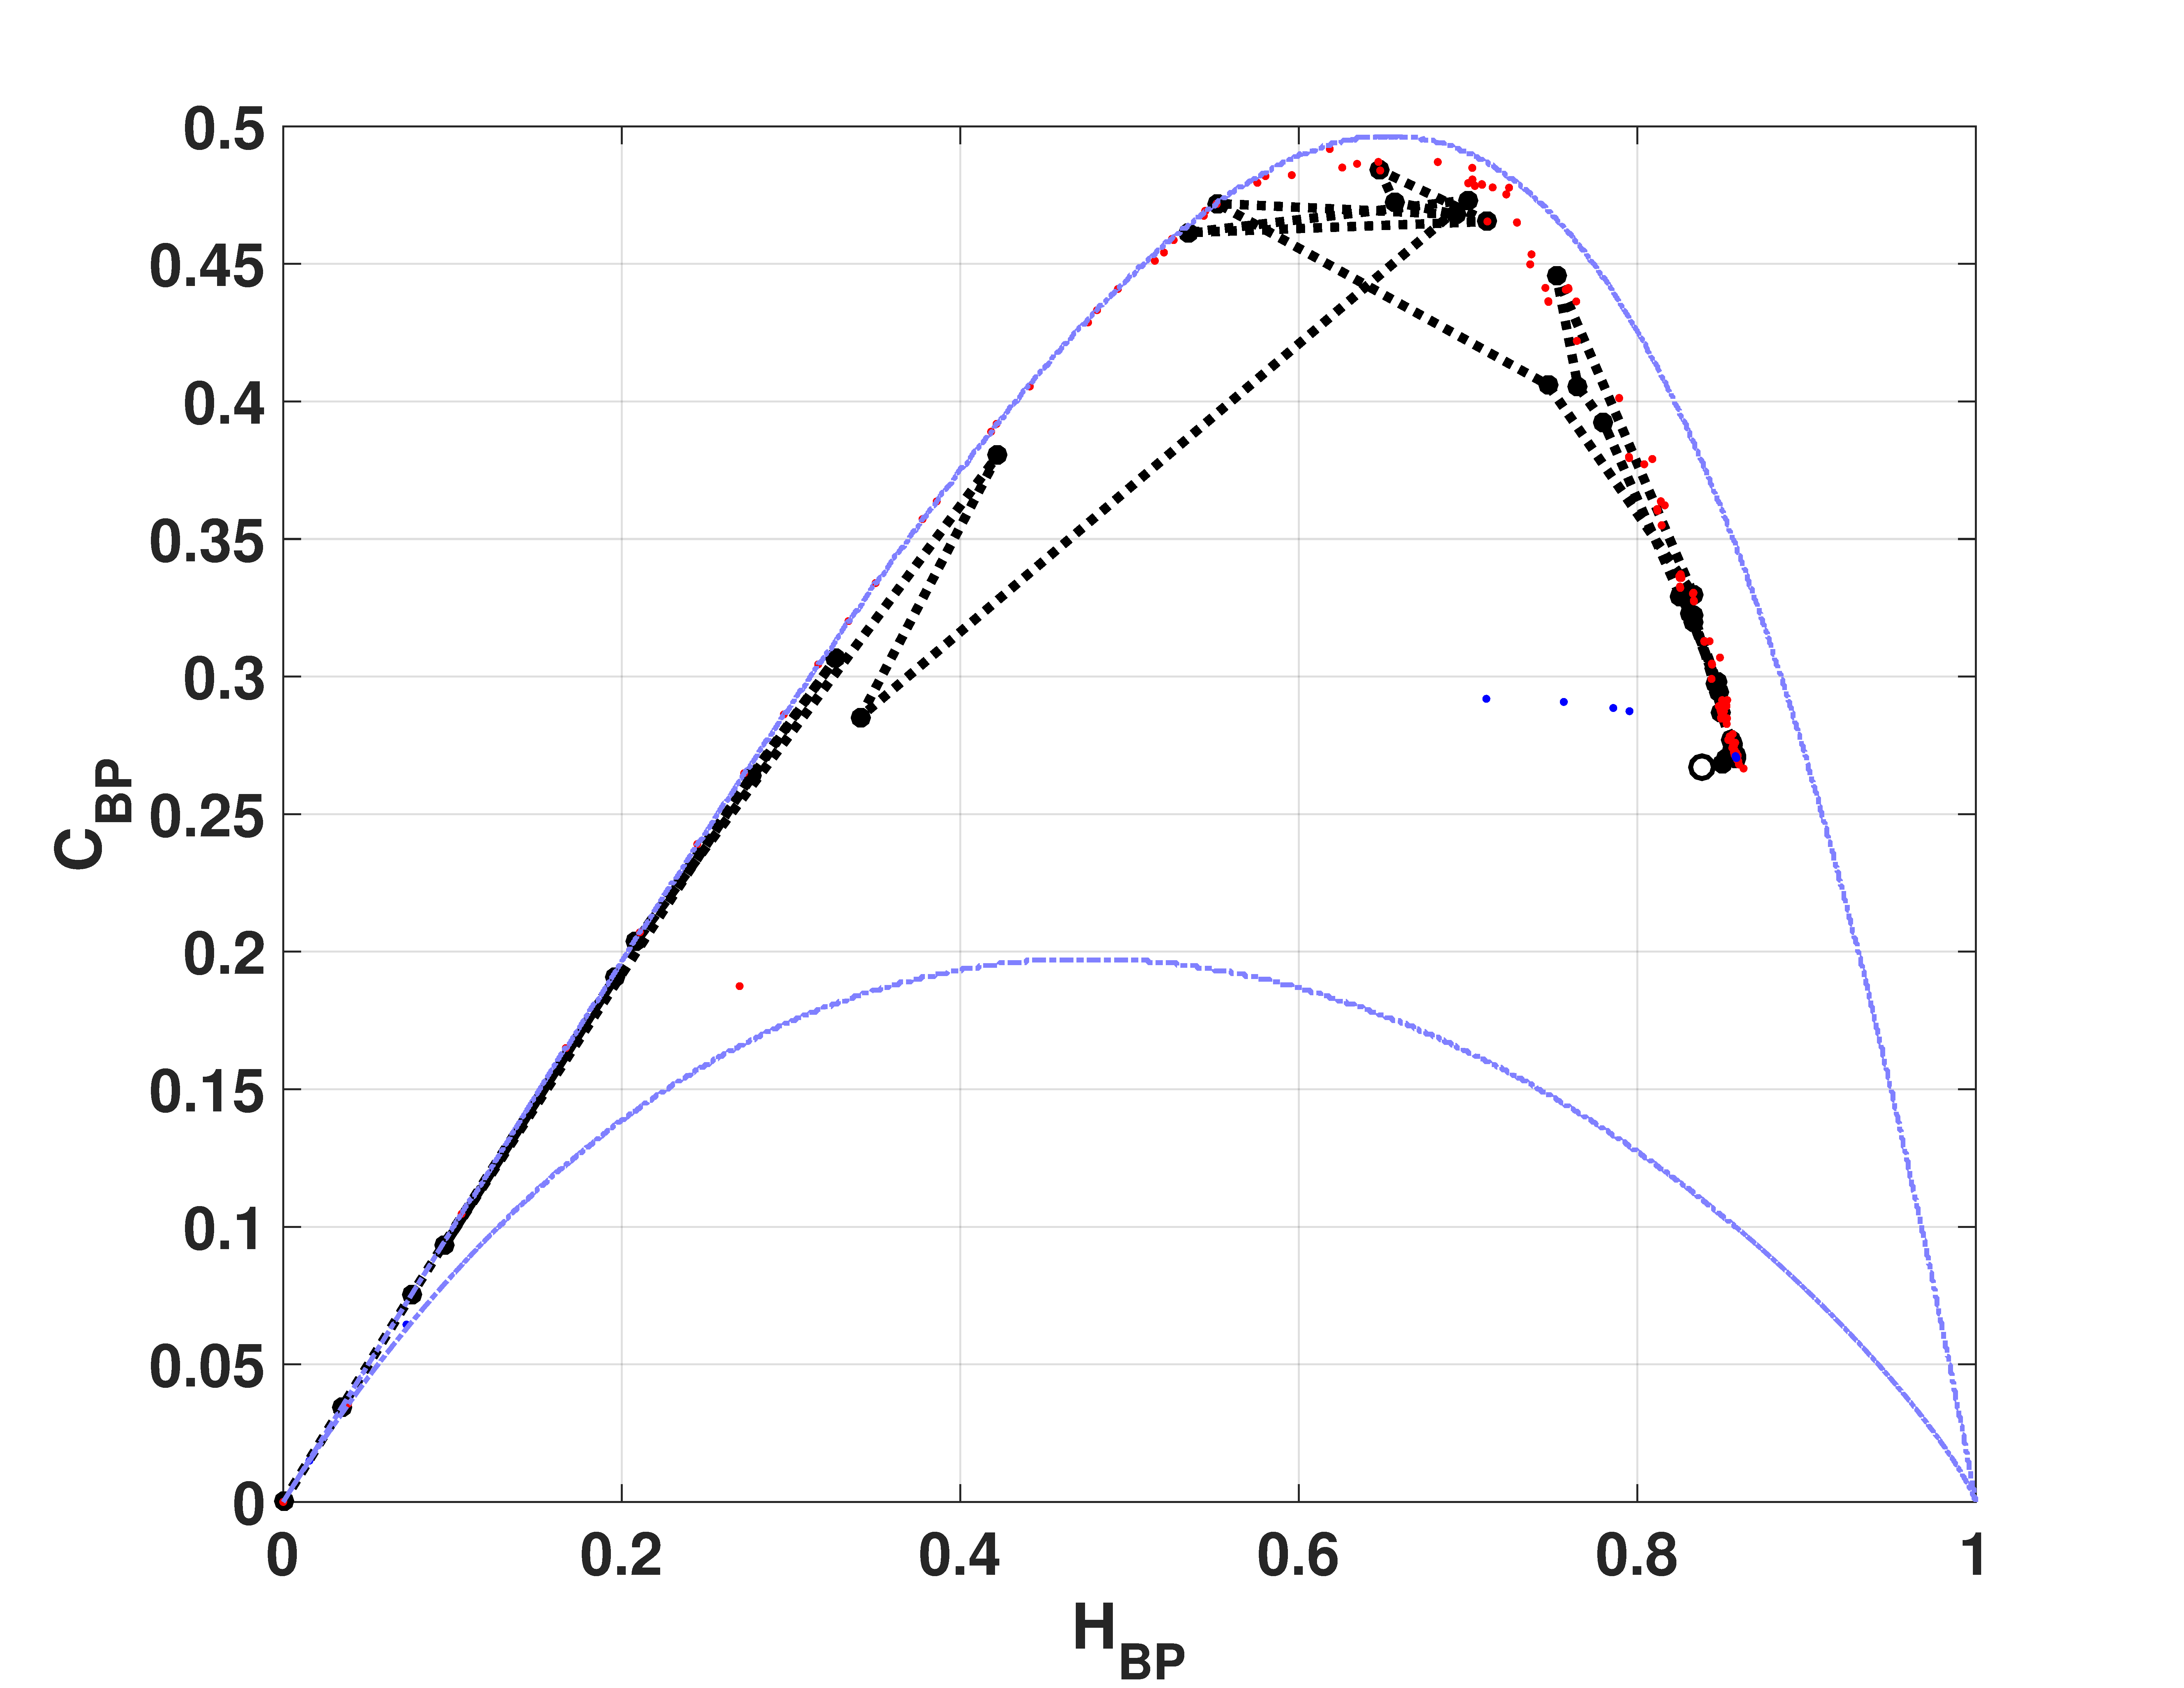
\includegraphics[width=.49\textwidth]{CbpHbp_SwitchEven}
	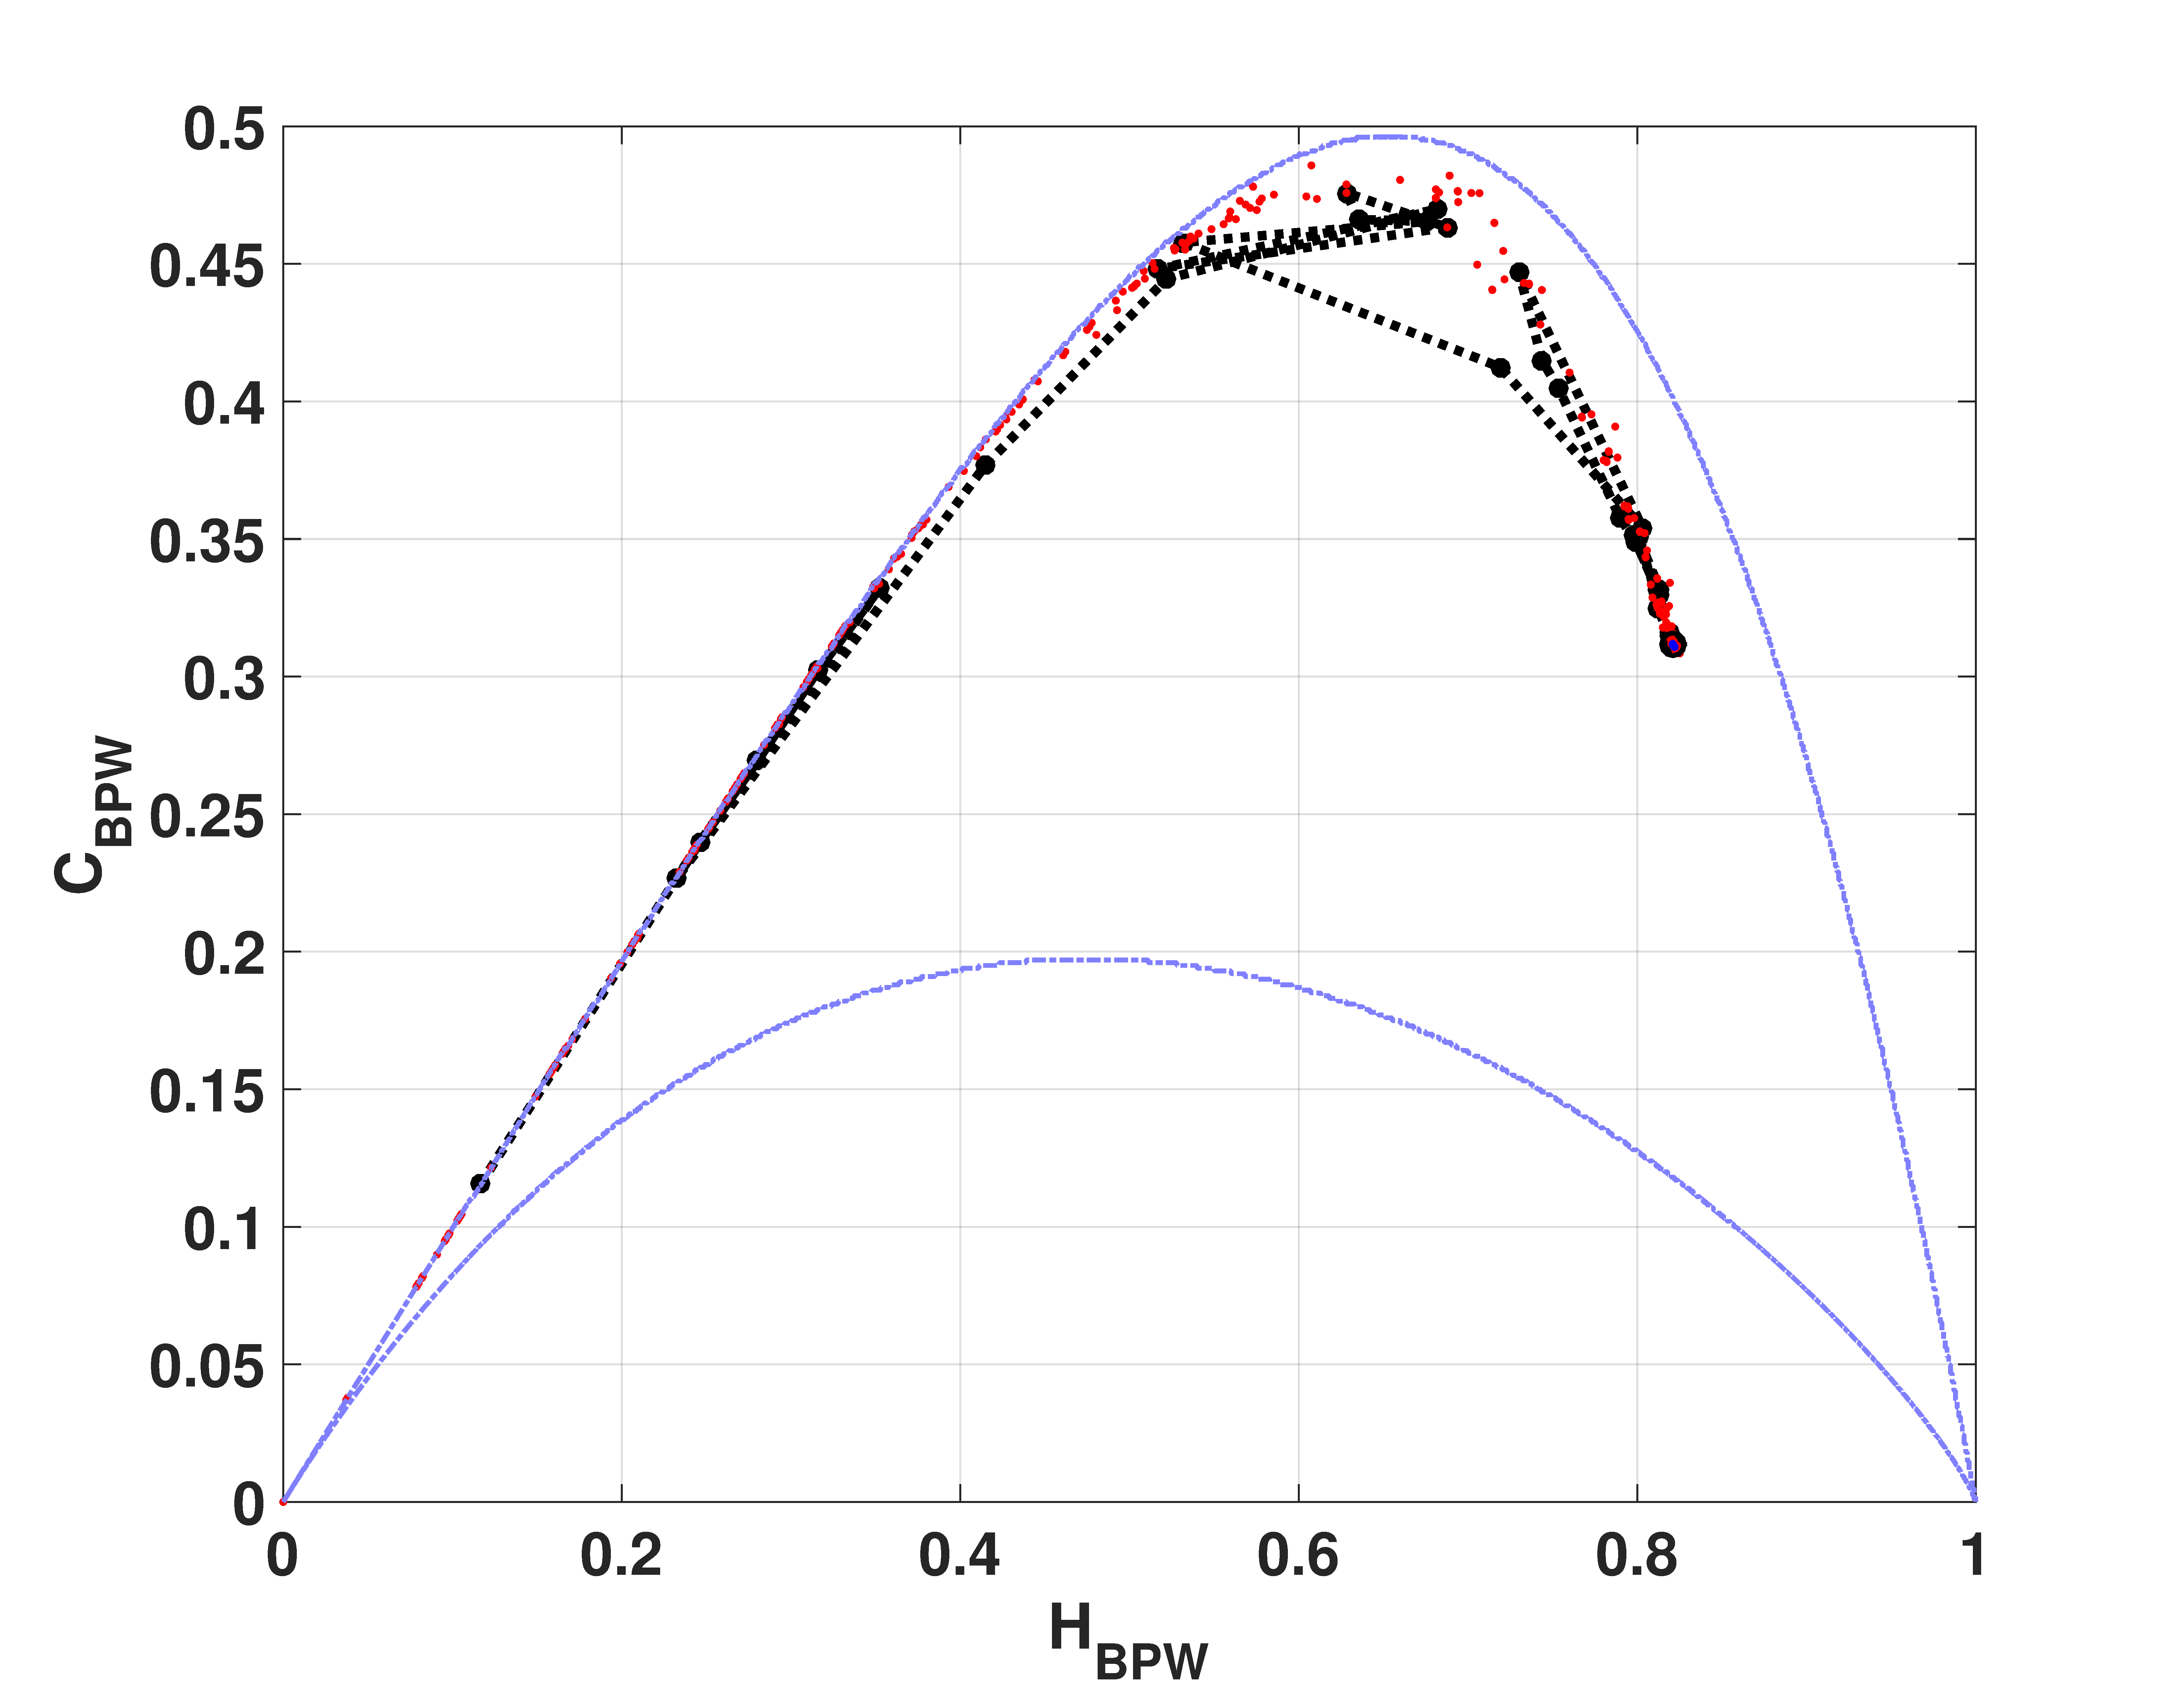
\includegraphics[width=.49\textwidth]{CbpwHbpw_SwitchEven}
	\caption{Evolution of statistical properties in entropy-complexity plane of LOG map using binary representation: (a) $C_{BP}$ vs $H_{BP}$ (b) $C_{BPW}$ vs $H_{BPW}$.}
	\label{fig:EVEN_HC}
\end{figure}

\begin{figure}
	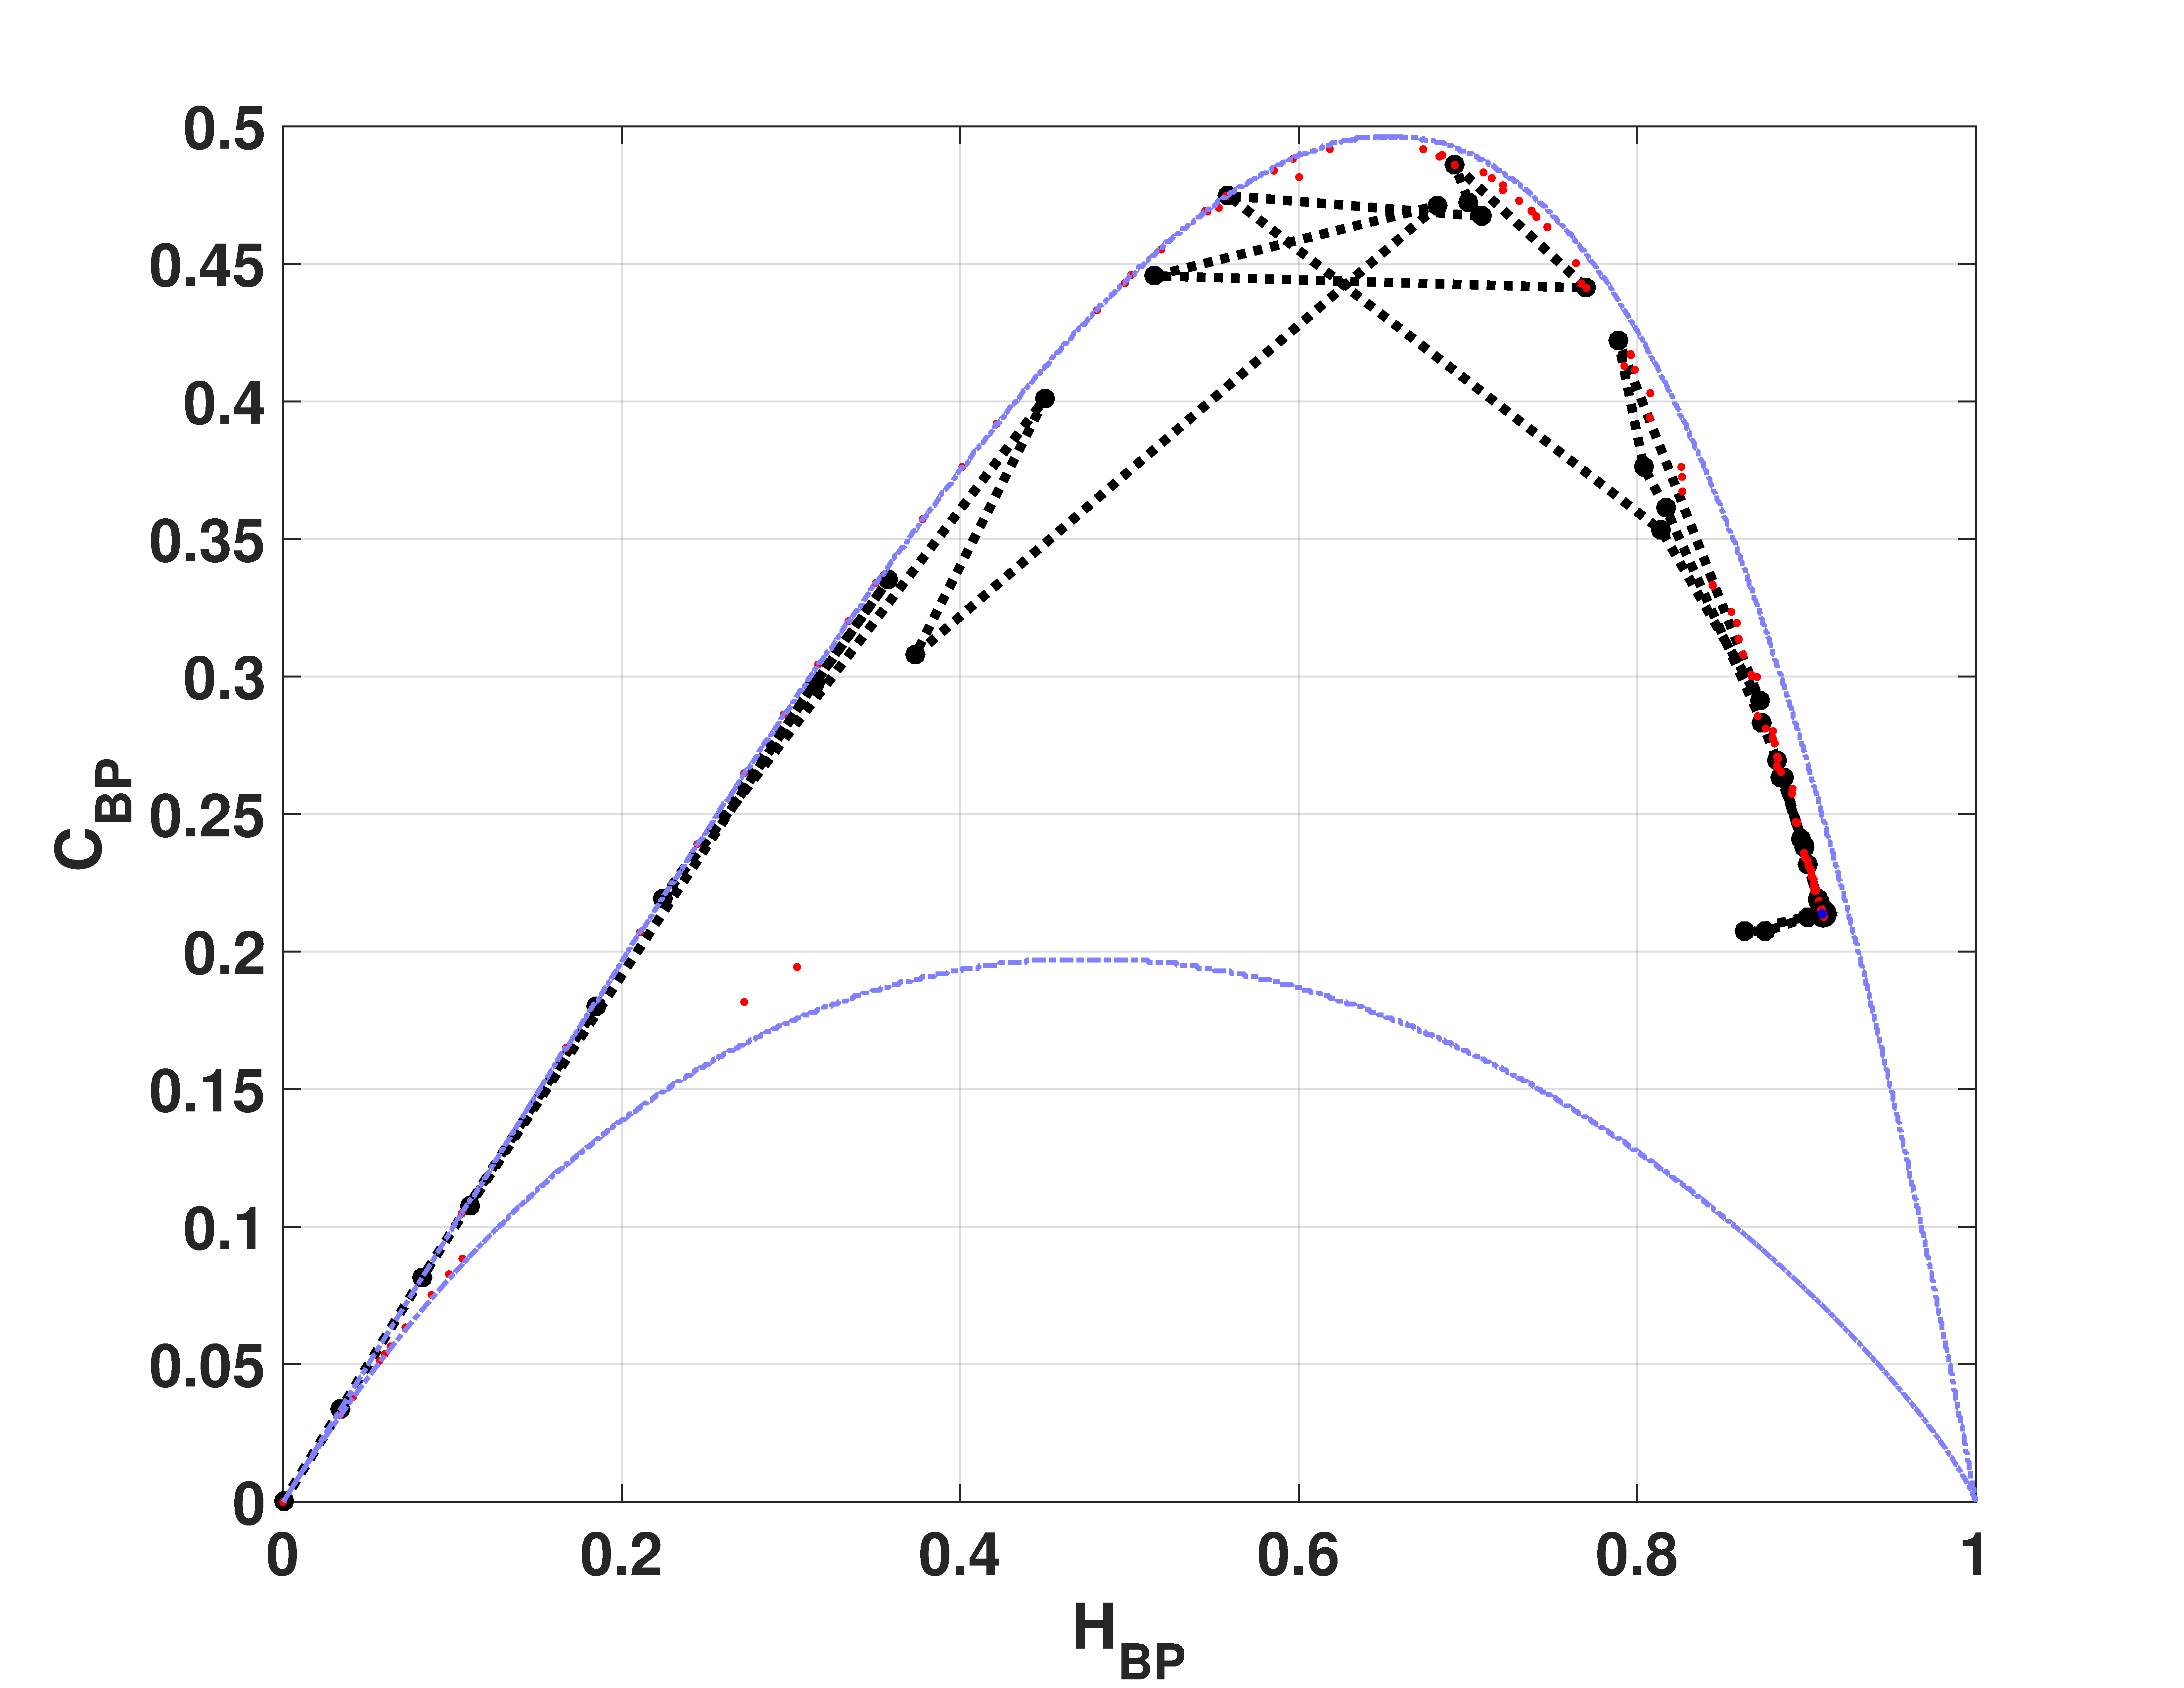
\includegraphics[width=.49\textwidth]{CbpHbp_SwitchOdd}
	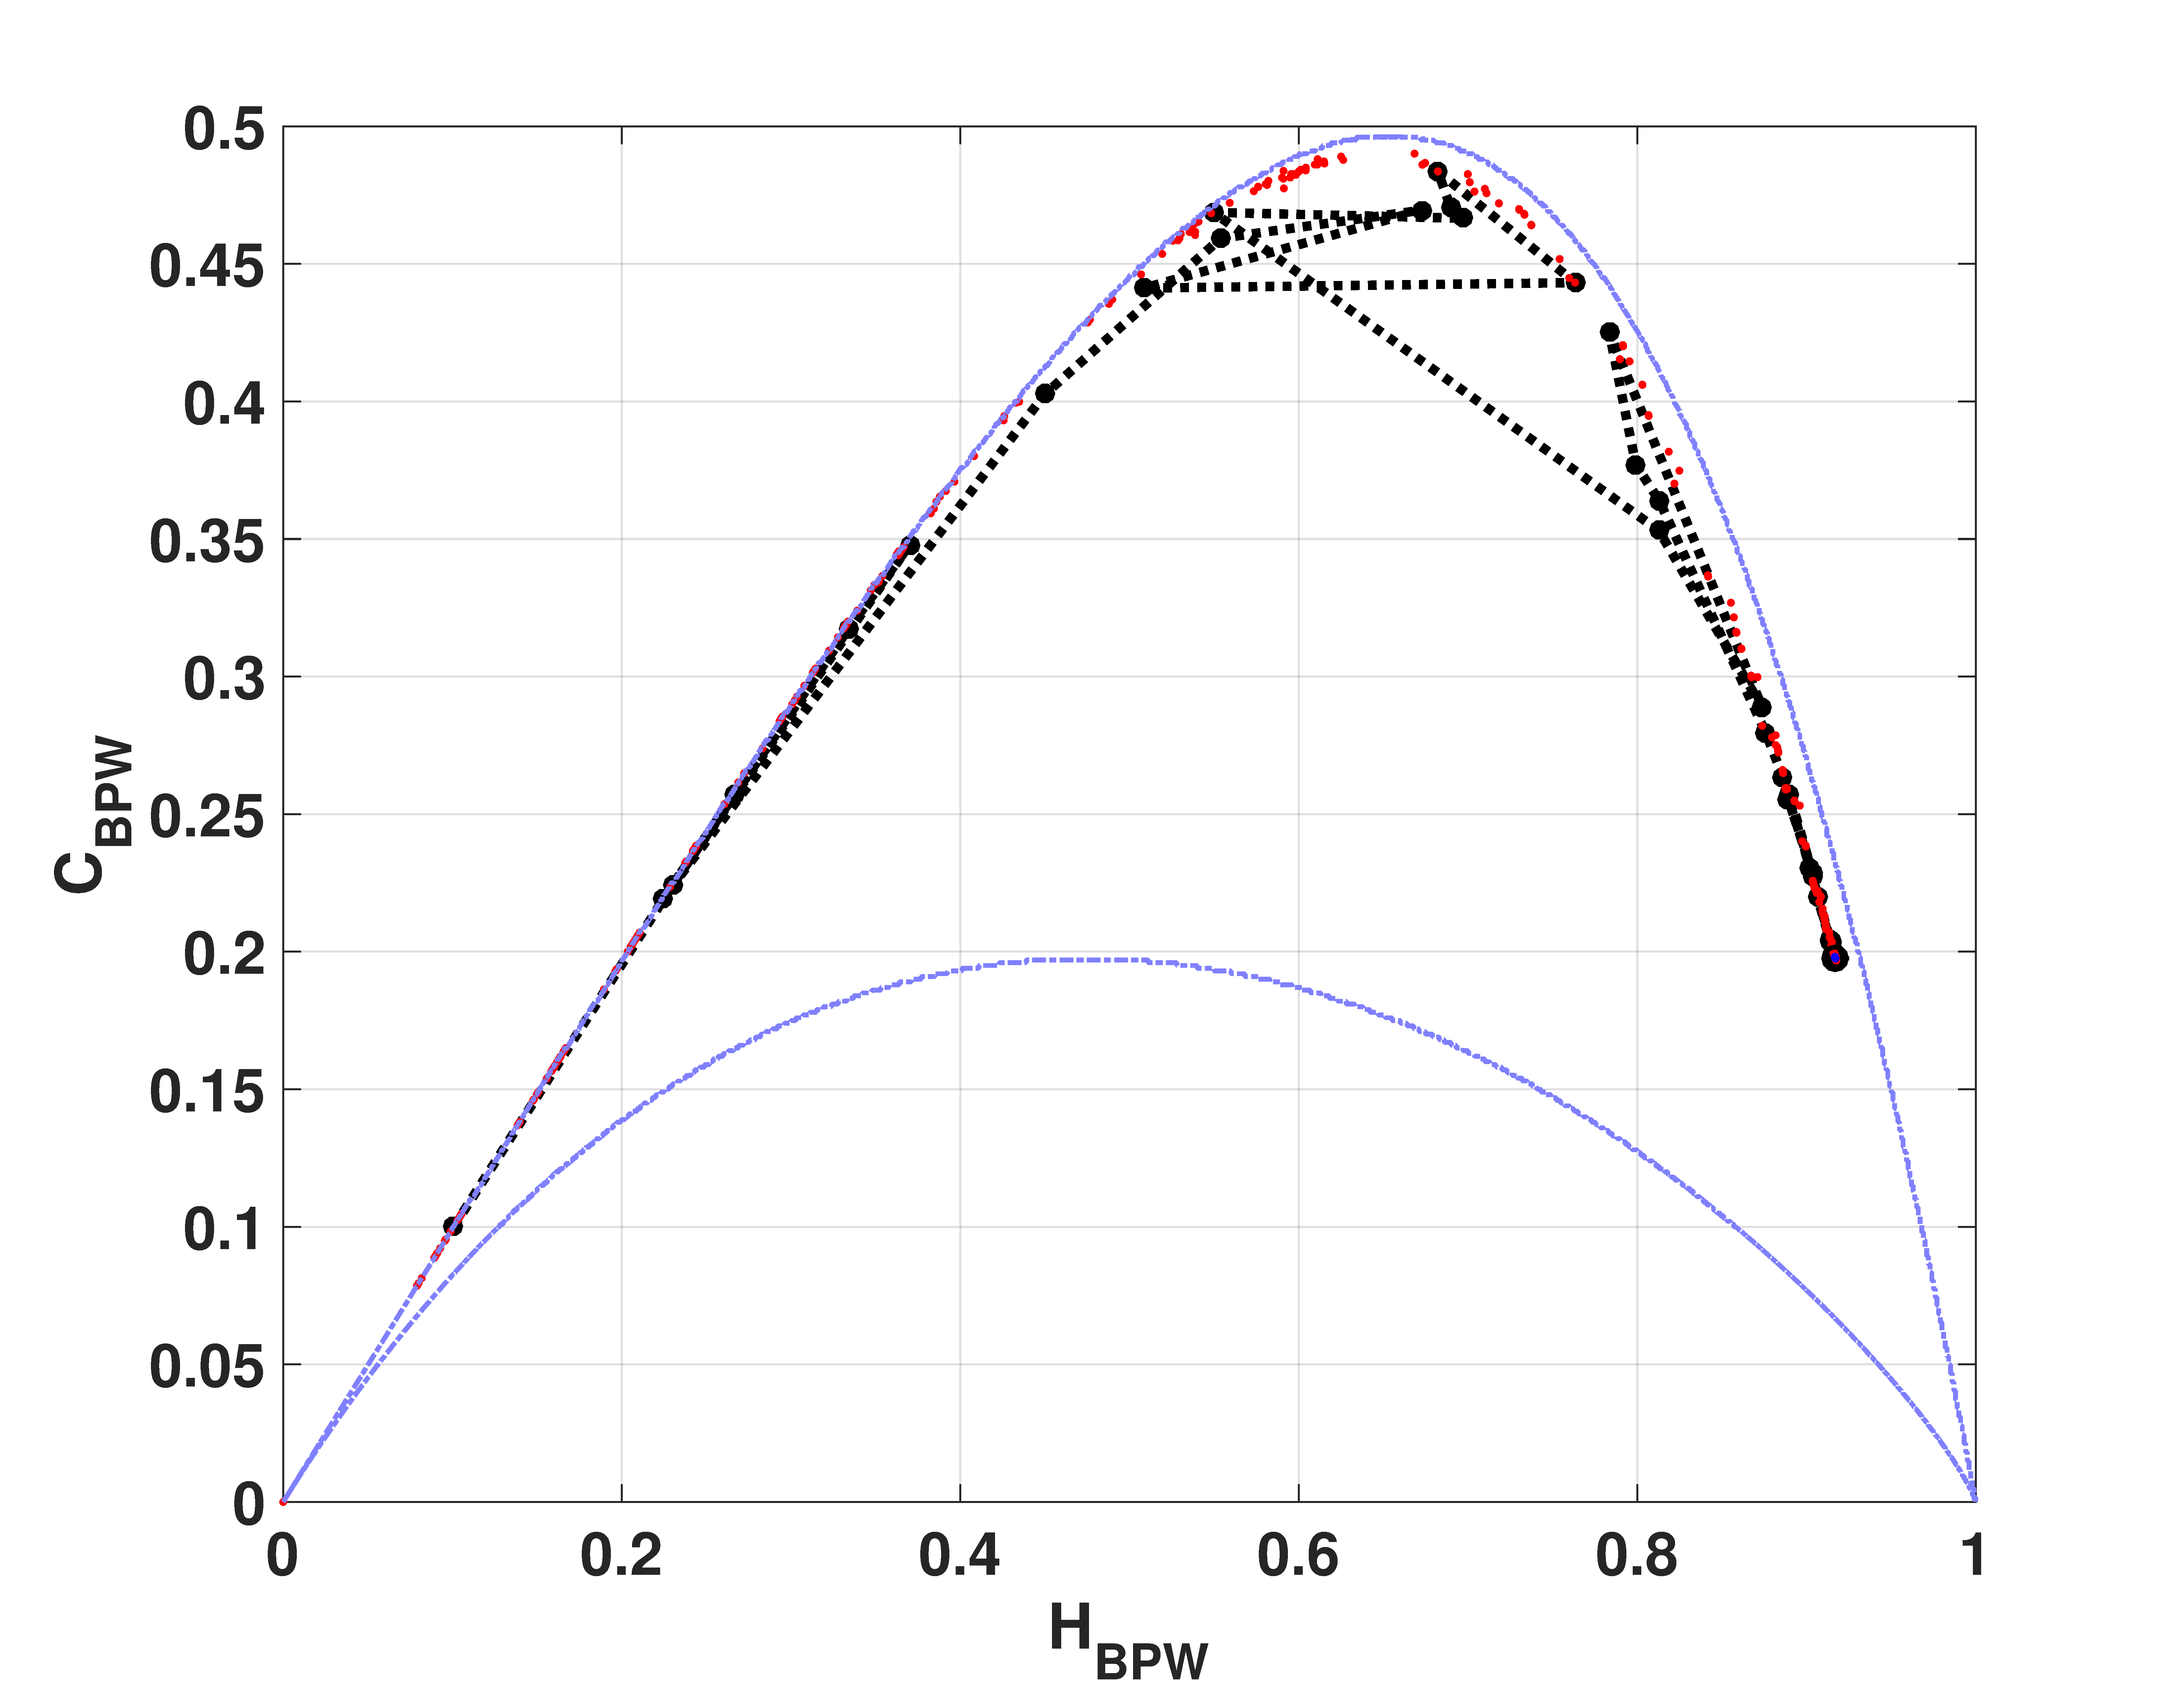
\includegraphics[width=.49\textwidth]{CbpwHbpw_SwitchOdd}
	\caption{Evolution of statistical properties in entropy-complexity plane of LOG map using binary representation: (a) $C_{BP}$ vs $H_{BP}$ (b) $C_{BPW}$ vs $H_{BPW}$.}
	\label{fig:ODD_HC}
\end{figure}